\documentclass[twoside]{book}

% Packages required by doxygen
\usepackage{fixltx2e}
\usepackage{calc}
\usepackage{doxygen}
\usepackage[export]{adjustbox} % also loads graphicx
\usepackage{graphicx}
\usepackage[utf8]{inputenc}
\usepackage{makeidx}
\usepackage{multicol}
\usepackage{multirow}
\PassOptionsToPackage{warn}{textcomp}
\usepackage{textcomp}
\usepackage[nointegrals]{wasysym}
\usepackage[table]{xcolor}

% Font selection
\usepackage[T1]{fontenc}
\usepackage[scaled=.90]{helvet}
\usepackage{courier}
\usepackage{amssymb}
\usepackage{sectsty}
\renewcommand{\familydefault}{\sfdefault}
\allsectionsfont{%
  \fontseries{bc}\selectfont%
  \color{darkgray}%
}
\renewcommand{\DoxyLabelFont}{%
  \fontseries{bc}\selectfont%
  \color{darkgray}%
}
\newcommand{\+}{\discretionary{\mbox{\scriptsize$\hookleftarrow$}}{}{}}

% Page & text layout
\usepackage{geometry}
\geometry{%
  a4paper,%
  top=2.5cm,%
  bottom=2.5cm,%
  left=2.5cm,%
  right=2.5cm%
}
\tolerance=750
\hfuzz=15pt
\hbadness=750
\setlength{\emergencystretch}{15pt}
\setlength{\parindent}{0cm}
\setlength{\parskip}{3ex plus 2ex minus 2ex}
\makeatletter
\renewcommand{\paragraph}{%
  \@startsection{paragraph}{4}{0ex}{-1.0ex}{1.0ex}{%
    \normalfont\normalsize\bfseries\SS@parafont%
  }%
}
\renewcommand{\subparagraph}{%
  \@startsection{subparagraph}{5}{0ex}{-1.0ex}{1.0ex}{%
    \normalfont\normalsize\bfseries\SS@subparafont%
  }%
}
\makeatother

% Headers & footers
\usepackage{fancyhdr}
\pagestyle{fancyplain}
\fancyhead[LE]{\fancyplain{}{\bfseries\thepage}}
\fancyhead[CE]{\fancyplain{}{}}
\fancyhead[RE]{\fancyplain{}{\bfseries\leftmark}}
\fancyhead[LO]{\fancyplain{}{\bfseries\rightmark}}
\fancyhead[CO]{\fancyplain{}{}}
\fancyhead[RO]{\fancyplain{}{\bfseries\thepage}}
\fancyfoot[LE]{\fancyplain{}{}}
\fancyfoot[CE]{\fancyplain{}{}}
\fancyfoot[RE]{\fancyplain{}{\bfseries\scriptsize Generated by Doxygen }}
\fancyfoot[LO]{\fancyplain{}{\bfseries\scriptsize Generated by Doxygen }}
\fancyfoot[CO]{\fancyplain{}{}}
\fancyfoot[RO]{\fancyplain{}{}}
\renewcommand{\footrulewidth}{0.4pt}
\renewcommand{\chaptermark}[1]{%
  \markboth{#1}{}%
}
\renewcommand{\sectionmark}[1]{%
  \markright{\thesection\ #1}%
}

% Indices & bibliography
\usepackage{natbib}
\usepackage[titles]{tocloft}
\setcounter{tocdepth}{3}
\setcounter{secnumdepth}{5}
\makeindex

% Hyperlinks (required, but should be loaded last)
\usepackage{ifpdf}
\ifpdf
  \usepackage[pdftex,pagebackref=true]{hyperref}
\else
  \usepackage[ps2pdf,pagebackref=true]{hyperref}
\fi
\hypersetup{%
  colorlinks=true,%
  linkcolor=blue,%
  citecolor=blue,%
  unicode%
}

% Custom commands
\newcommand{\clearemptydoublepage}{%
  \newpage{\pagestyle{empty}\cleardoublepage}%
}

\usepackage{caption}
\captionsetup{labelsep=space,justification=centering,font={bf},singlelinecheck=off,skip=4pt,position=top}

%===== C O N T E N T S =====

\begin{document}

% Titlepage & ToC
\hypersetup{pageanchor=false,
             bookmarksnumbered=true,
             pdfencoding=unicode
            }
\pagenumbering{alph}
\begin{titlepage}
\vspace*{7cm}
\begin{center}%
{\Large Galaxy\+Lib-\/\+P\+HP \\[1ex]\large v0.\+1 }\\
\vspace*{1cm}
{\large Generated by Doxygen 1.8.12}\\
\end{center}
\end{titlepage}
\clearemptydoublepage
\pagenumbering{roman}
\tableofcontents
\clearemptydoublepage
\pagenumbering{arabic}
\hypersetup{pageanchor=true}

%--- Begin generated contents ---
\chapter{Module Index}
\section{Modules}
Here is a list of all modules\+:\begin{DoxyCompactList}
\item \contentsline{section}{Data\+Types class}{\pageref{group__data__types__class}}{}
\item \contentsline{section}{Folder\+Contents class}{\pageref{group__folder__contents__class}}{}
\item \contentsline{section}{Folders class}{\pageref{group__folders__class}}{}
\item \contentsline{section}{Galaxy\+Instance Class}{\pageref{group__galaxy__instance__class}}{}
\item \contentsline{section}{genome Class}{\pageref{group__genomes__class}}{}
\item \contentsline{section}{Groups\+Roles Class}{\pageref{group__group__roles__class}}{}
\item \contentsline{section}{Groups Class}{\pageref{group__group__class}}{}
\item \contentsline{section}{Group\+Users Class}{\pageref{group__group__users__class}}{}
\item \contentsline{section}{Histories class}{\pageref{group__histories__class}}{}
\item \contentsline{section}{History\+Contents class}{\pageref{group__history__contents__class}}{}
\item \contentsline{section}{H\+T\+T\+P\+Request Class}{\pageref{group__http__request__class}}{}
\item \contentsline{section}{Jobs}{\pageref{group__Jobs}}{}
\item \contentsline{section}{Folders class}{\pageref{group__libraries__class}}{}
\item \contentsline{section}{Request\+Error}{\pageref{group__request__error__class}}{}
\item \contentsline{section}{Request}{\pageref{group__request__class}}{}
\item \contentsline{section}{roels Class}{\pageref{group__roles__class}}{}
\item \contentsline{section}{Search Class}{\pageref{group__search__class}}{}
\item \contentsline{section}{tools Class}{\pageref{group__tools__class}}{}
\item \contentsline{section}{Tool Shed Repositories}{\pageref{group__tool__shed__repositories__class}}{}
\item \contentsline{section}{Users Class}{\pageref{group__users__class}}{}
\item \contentsline{section}{Visualizations Class}{\pageref{group__visualizations__class}}{}
\end{DoxyCompactList}

\chapter{Hierarchical Index}
\section{Class Hierarchy}
This inheritance list is sorted roughly, but not completely, alphabetically\-:\begin{DoxyCompactList}
\item \contentsline{section}{Galaxy\-Datasets}{\pageref{classGalaxyDatasets}}{}
\item \contentsline{section}{Galaxy\-Datatypes}{\pageref{classGalaxyDatatypes}}{}
\item \contentsline{section}{Galaxy\-Error}{\pageref{classGalaxyError}}{}
\item \contentsline{section}{Galaxy\-Folder\-Contents}{\pageref{classGalaxyFolderContents}}{}
\item \contentsline{section}{Galaxy\-Folders}{\pageref{classGalaxyFolders}}{}
\item \contentsline{section}{Galaxy\-Genomes}{\pageref{classGalaxyGenomes}}{}
\item \contentsline{section}{Galaxy\-Group\-Roles}{\pageref{classGalaxyGroupRoles}}{}
\item \contentsline{section}{Galaxy\-Groups}{\pageref{classGalaxyGroups}}{}
\item \contentsline{section}{Galaxy\-Group\-Users}{\pageref{classGalaxyGroupUsers}}{}
\item \contentsline{section}{Galaxy\-Histories}{\pageref{classGalaxyHistories}}{}
\item \contentsline{section}{Galaxy\-History\-Contents}{\pageref{classGalaxyHistoryContents}}{}
\item \contentsline{section}{Galaxy\-H\-T\-T\-P\-Request}{\pageref{classGalaxyHTTPRequest}}{}
\begin{DoxyCompactList}
\item \contentsline{section}{Galaxy\-Instance}{\pageref{classGalaxyInstance}}{}
\end{DoxyCompactList}
\item \contentsline{section}{Galaxy\-Jobs}{\pageref{classGalaxyJobs}}{}
\item \contentsline{section}{Galaxy\-Libraries}{\pageref{classGalaxyLibraries}}{}
\item \contentsline{section}{Galaxy\-Library\-Contents}{\pageref{classGalaxyLibraryContents}}{}
\item \contentsline{section}{Galaxy\-Requests}{\pageref{classGalaxyRequests}}{}
\item \contentsline{section}{Galaxy\-Roles}{\pageref{classGalaxyRoles}}{}
\item \contentsline{section}{Galaxy\-Search}{\pageref{classGalaxySearch}}{}
\item \contentsline{section}{Galaxy\-Tools}{\pageref{classGalaxyTools}}{}
\item \contentsline{section}{Galaxy\-Tool\-Shed\-Repositories}{\pageref{classGalaxyToolShedRepositories}}{}
\item \contentsline{section}{Galaxy\-Users}{\pageref{classGalaxyUsers}}{}
\item \contentsline{section}{Galaxy\-Visualizations}{\pageref{classGalaxyVisualizations}}{}
\item \contentsline{section}{Galaxy\-Workflows}{\pageref{classGalaxyWorkflows}}{}
\end{DoxyCompactList}

\chapter{Class Index}
\section{Class List}
Here are the classes, structs, unions and interfaces with brief descriptions\+:\begin{DoxyCompactList}
\item\contentsline{section}{\hyperlink{classDatasets}{Datasets} }{\pageref{classDatasets}}{}
\item\contentsline{section}{\hyperlink{classDatatypes}{Datatypes} }{\pageref{classDatatypes}}{}
\item\contentsline{section}{\hyperlink{classFolderContents}{Folder\+Contents} }{\pageref{classFolderContents}}{}
\item\contentsline{section}{\hyperlink{classFolders}{Folders} }{\pageref{classFolders}}{}
\item\contentsline{section}{\hyperlink{classGalaxyInstance}{Galaxy\+Instance} }{\pageref{classGalaxyInstance}}{}
\item\contentsline{section}{\hyperlink{classGenomes}{Genomes} }{\pageref{classGenomes}}{}
\item\contentsline{section}{\hyperlink{classGroupRoles}{Group\+Roles} }{\pageref{classGroupRoles}}{}
\item\contentsline{section}{\hyperlink{classGroups}{Groups} }{\pageref{classGroups}}{}
\item\contentsline{section}{\hyperlink{classGroupUsers}{Group\+Users} }{\pageref{classGroupUsers}}{}
\item\contentsline{section}{\hyperlink{classHistories}{Histories} }{\pageref{classHistories}}{}
\item\contentsline{section}{\hyperlink{classHistoryContents}{History\+Contents} }{\pageref{classHistoryContents}}{}
\item\contentsline{section}{\hyperlink{classHTTPRequest}{H\+T\+T\+P\+Request} }{\pageref{classHTTPRequest}}{}
\item\contentsline{section}{\hyperlink{classJobs}{Jobs} }{\pageref{classJobs}}{}
\item\contentsline{section}{\hyperlink{classLibraries}{Libraries} }{\pageref{classLibraries}}{}
\item\contentsline{section}{\hyperlink{classLibraryContents}{Library\+Contents} }{\pageref{classLibraryContents}}{}
\item\contentsline{section}{\hyperlink{classRequestError}{Request\+Error} }{\pageref{classRequestError}}{}
\item\contentsline{section}{\hyperlink{classRequests}{Requests} }{\pageref{classRequests}}{}
\item\contentsline{section}{\hyperlink{classRoles}{Roles} }{\pageref{classRoles}}{}
\item\contentsline{section}{\hyperlink{classSearch}{Search} }{\pageref{classSearch}}{}
\item\contentsline{section}{\hyperlink{classTools}{Tools} }{\pageref{classTools}}{}
\item\contentsline{section}{\hyperlink{classToolShedRepositories}{Tool\+Shed\+Repositories} }{\pageref{classToolShedRepositories}}{}
\item\contentsline{section}{\hyperlink{classUsers}{Users} }{\pageref{classUsers}}{}
\item\contentsline{section}{\hyperlink{classVisualizations}{Visualizations} }{\pageref{classVisualizations}}{}
\item\contentsline{section}{\hyperlink{classWorkflows}{Workflows} }{\pageref{classWorkflows}}{}
\end{DoxyCompactList}

\chapter{File Index}
\section{File List}
Here is a list of all documented files with brief descriptions\+:\begin{DoxyCompactList}
\item\contentsline{section}{\hyperlink{DataSets_8inc}{Data\+Sets.\+inc} }{\pageref{DataSets_8inc}}{}
\item\contentsline{section}{\hyperlink{DataTypes_8inc}{Data\+Types.\+inc} }{\pageref{DataTypes_8inc}}{}
\item\contentsline{section}{\hyperlink{FolderContents_8inc}{Folder\+Contents.\+inc} }{\pageref{FolderContents_8inc}}{}
\item\contentsline{section}{\hyperlink{Folders_8inc}{Folders.\+inc} }{\pageref{Folders_8inc}}{}
\item\contentsline{section}{\hyperlink{GalaxyInstance_8inc}{Galaxy\+Instance.\+inc} }{\pageref{GalaxyInstance_8inc}}{}
\item\contentsline{section}{\hyperlink{Genomes_8inc}{Genomes.\+inc} }{\pageref{Genomes_8inc}}{}
\item\contentsline{section}{\hyperlink{GroupRoles_8inc}{Group\+Roles.\+inc} }{\pageref{GroupRoles_8inc}}{}
\item\contentsline{section}{\hyperlink{Groups_8inc}{Groups.\+inc} }{\pageref{Groups_8inc}}{}
\item\contentsline{section}{\hyperlink{GroupUsers_8inc}{Group\+Users.\+inc} }{\pageref{GroupUsers_8inc}}{}
\item\contentsline{section}{\hyperlink{Histories_8inc}{Histories.\+inc} }{\pageref{Histories_8inc}}{}
\item\contentsline{section}{\hyperlink{HistoryContents_8inc}{History\+Contents.\+inc} }{\pageref{HistoryContents_8inc}}{}
\item\contentsline{section}{\hyperlink{HTTPRequest_8inc}{H\+T\+T\+P\+Request.\+inc} }{\pageref{HTTPRequest_8inc}}{}
\item\contentsline{section}{\hyperlink{Jobs_8inc}{Jobs.\+inc} }{\pageref{Jobs_8inc}}{}
\item\contentsline{section}{\hyperlink{Libraries_8inc}{Libraries.\+inc} }{\pageref{Libraries_8inc}}{}
\item\contentsline{section}{\hyperlink{RequestError_8inc}{Request\+Error.\+inc} }{\pageref{RequestError_8inc}}{}
\item\contentsline{section}{\hyperlink{Requests_8inc}{Requests.\+inc} }{\pageref{Requests_8inc}}{}
\item\contentsline{section}{\hyperlink{Roles_8inc}{Roles.\+inc} }{\pageref{Roles_8inc}}{}
\item\contentsline{section}{\hyperlink{Search_8inc}{Search.\+inc} }{\pageref{Search_8inc}}{}
\item\contentsline{section}{\hyperlink{Tools_8inc}{Tools.\+inc} }{\pageref{Tools_8inc}}{}
\item\contentsline{section}{\hyperlink{ToolShedRepositories_8inc}{Tool\+Shed\+Repositories.\+inc} }{\pageref{ToolShedRepositories_8inc}}{}
\item\contentsline{section}{\hyperlink{Users_8inc}{Users.\+inc} }{\pageref{Users_8inc}}{}
\item\contentsline{section}{\hyperlink{Visualizations_8inc}{Visualizations.\+inc} }{\pageref{Visualizations_8inc}}{}
\item\contentsline{section}{\hyperlink{Workflows_8inc}{Workflows.\+inc} }{\pageref{Workflows_8inc}}{}
\end{DoxyCompactList}

\chapter{Module Documentation}
\hypertarget{group__data__types__class}{}\section{Data\+Types class}
\label{group__data__types__class}\index{Data\+Types class@{Data\+Types class}}
The Data\+Types Class interacts with Galaxy to manage Data\+Types. The functions in this class correspond to the Galaxy A\+PI functions and are named similarly to their Python counterpart. 
\hypertarget{group__folder__contents__class}{}\section{Folder\+Contents class}
\label{group__folder__contents__class}\index{Folder\+Contents class@{Folder\+Contents class}}
The folder contents Class interacts with Galaxy to manage content of folders. The functions in this class correspond to the Galaxy A\+PI functions and are named similarly to their Python counterpart. 
\hypertarget{group__folders__class}{}\section{Folders class}
\label{group__folders__class}\index{Folders class@{Folders class}}
The folders Class interacts with Galaxy to manage its folders. The functions in this class correspond to the Galaxy A\+PI functions and are named similarly to their Python counterpart. 
\hypertarget{group__galaxy__instance__class}{}\section{Galaxy\+Instance Class}
\label{group__galaxy__instance__class}\index{Galaxy\+Instance Class@{Galaxy\+Instance Class}}
The \hyperlink{classGalaxyInstance}{Galaxy\+Instance} class is used to connect to a remote Galaxy server. It authenticates and maintains the A\+PI key for the user. The functions in this class correspond to the Galaxy A\+PI functions and are named similarly to their Python counterpart. 
\hypertarget{group__genomes__class}{}\section{genome Class}
\label{group__genomes__class}\index{genome Class@{genome Class}}
The \hyperlink{classGenomes}{Genomes} class interacts with Galaxy to manage contents of a Galaxy Genome. The functions in this class correspond to the Galaxy A\+PI functions and are named similarly to their Python counterparts. 
\hypertarget{group__group__roles__class}{}\section{Groups\+Roles Class}
\label{group__group__roles__class}\index{Groups\+Roles Class@{Groups\+Roles Class}}
The \hyperlink{classGroupRoles}{Group\+Roles} Class interacts with Galaxy to manage user groups and roles. The functions in this class correspond to the Galaxy A\+PI functions and are named similarly to their Python counterpart. 
\hypertarget{group__group__class}{}\section{Groups Class}
\label{group__group__class}\index{Groups Class@{Groups Class}}
The Group Class interacts with Galaxy to manage user groups and roles. The functions in this class correspond to the Galaxy A\+PI functions and are named similarly to their Python counterpart. 
\hypertarget{group__group__users__class}{}\section{Group\+Users Class}
\label{group__group__users__class}\index{Group\+Users Class@{Group\+Users Class}}
The \hyperlink{classGroupUsers}{Group\+Users} Class interacts with Galaxy to manage users of groups. The functions in this class correspond to the Galaxy A\+PI functions and are named similarly to their Python counterpart. 
\hypertarget{group__histories__class}{}\section{Histories class}
\label{group__histories__class}\index{Histories class@{Histories class}}
The \hyperlink{classHistories}{Histories} Class interacts with Galaxy to manage history data. The functions in this class correspond to the Galaxy A\+PI functions and are named similarly to their Python counterpart. 
\hypertarget{group__history__contents__class}{}\section{History\+Contents class}
\label{group__history__contents__class}\index{History\+Contents class@{History\+Contents class}}
The \hyperlink{classHistories}{Histories} Class interacts with Galaxy to manage history data. The functions in this class correspond to the Galaxy A\+PI functions and are named similarly to their Python counterpart. 
\hypertarget{group__http__request__class}{}\section{H\+T\+T\+P\+Request Class}
\label{group__http__request__class}\index{H\+T\+T\+P\+Request Class@{H\+T\+T\+P\+Request Class}}
The \hyperlink{classHTTPRequest}{H\+T\+T\+P\+Request} Class contains methods for using C\+U\+RL rest options. More specifically, U\+P\+D\+A\+TE, P\+O\+ST, D\+E\+L\+E\+TE, P\+UT and G\+ET. 
\hypertarget{group__Jobs}{}\section{Jobs}
\label{group__Jobs}\index{Jobs@{Jobs}}
The \hyperlink{classJobs}{Jobs} Class interacts with Galaxy to manage its folders. The functions in this class correspond to the Galaxy A\+PI functions and are named similarly to their Python counterpart. 
\hypertarget{group__libraries__class}{}\section{Folders class}
\label{group__libraries__class}\index{Folders class@{Folders class}}
The libraries Class interacts with Galaxy to manage its libraries. The functions in this class correspond to the Galaxy A\+PI functions and are named similarly to their Python counterpart. 
\hypertarget{group__request__error__class}{}\section{Request\+Error}
\label{group__request__error__class}\index{Request\+Error@{Request\+Error}}
The Request Error class dedicated to relaying error information given from a curl server response. 
\hypertarget{group__request__class}{}\section{Request}
\label{group__request__class}\index{Request@{Request}}
A class Built to manage basic Galaxy R\+E\+ST request options. 
\hypertarget{group__roles__class}{}\section{roels Class}
\label{group__roles__class}\index{roels Class@{roels Class}}
The \hyperlink{classRoles}{Roles} class interacts with Galaxy to manage contents of a Galaxy role. The functions in this class correspond to the Galaxy A\+PI functions and are named similarly to their Python counterparts. 
\hypertarget{group__search__class}{}\section{Search Class}
\label{group__search__class}\index{Search Class@{Search Class}}
The \hyperlink{classSearch}{Search} class contains a method for quering S\+QL searches accross Galaxy tables. This class corresponds to its Galaxy A\+PI equivalent and is named similarly. 
\hypertarget{group__tools__class}{}\section{tools Class}
\label{group__tools__class}\index{tools Class@{tools Class}}
The tools class interacts with Galaxy to manage contents of a Galaxy tool. The functions in this class correspond to the Galaxy A\+PI functions and are named similarly to their Python counterparts. 
\hypertarget{group__tool__shed__repositories__class}{}\section{Tool Shed Repositories}
\label{group__tool__shed__repositories__class}\index{Tool Shed Repositories@{Tool Shed Repositories}}
The tool shed repositories class interacts with Galaxy to manage contents regarding its tool shed repositories. The functions in this class correspond to the Galaxy A\+PI functions and are named similarly to their Python counterparts. 
\hypertarget{group__users__class}{}\section{Users Class}
\label{group__users__class}\index{Users Class@{Users Class}}
The \hyperlink{classUsers}{Users} class interacts with Galaxy to manage contents of a Galaxy user. The functions in this class correspond to the Galaxy A\+PI functions and are named similarly to their Python counterparts. 
\hypertarget{group__visualizations__class}{}\section{Visualizations Class}
\label{group__visualizations__class}\index{Visualizations Class@{Visualizations Class}}
The Visualization class interacts with Galaxy to manage contents of a Galaxy visualization. The functions in this class correspond to the Galaxy A\+PI functions and are named similarly to their Python counterparts. 
\chapter{Class Documentation}
\hypertarget{classDatasets}{}\section{Datasets Class Reference}
\label{classDatasets}\index{Datasets@{Datasets}}
Inheritance diagram for Datasets\+:\begin{figure}[H]
\begin{center}
\leavevmode
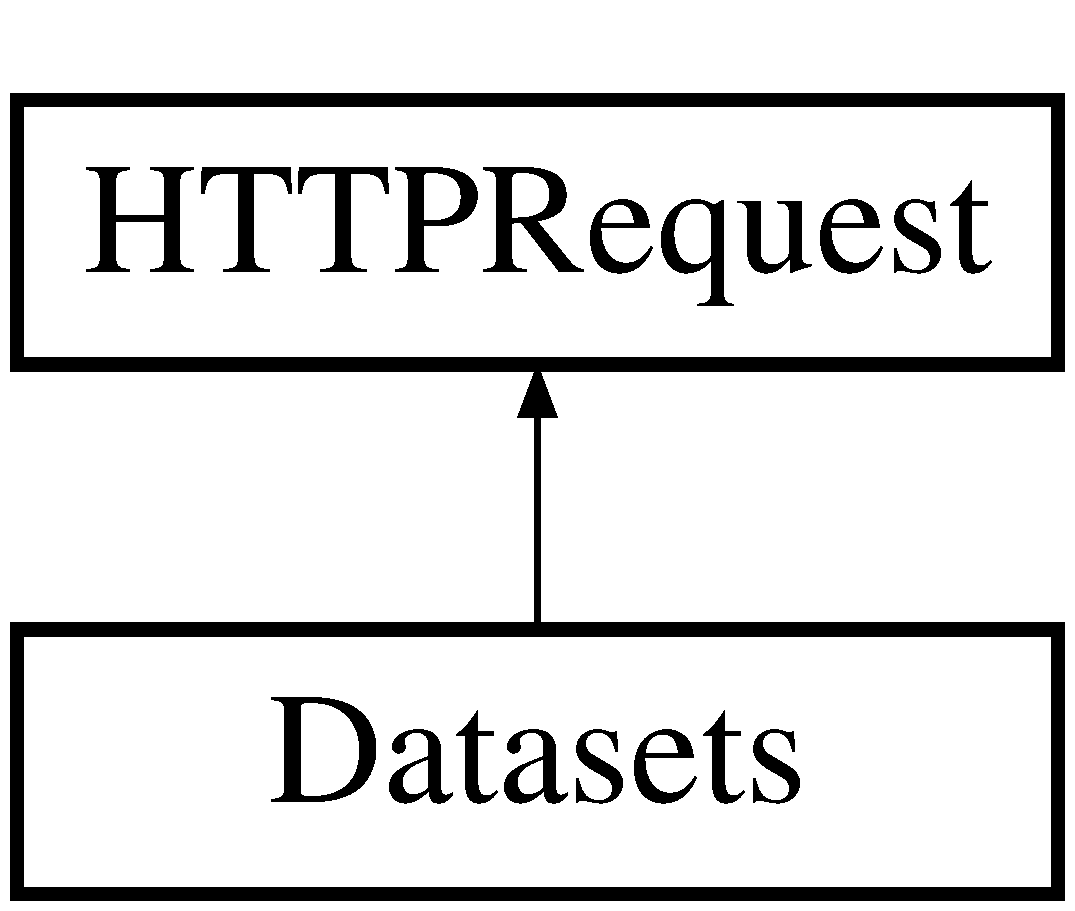
\includegraphics[height=2.000000cm]{classDatasets}
\end{center}
\end{figure}
\subsection*{Public Member Functions}
\begin{DoxyCompactItemize}
\item 
\hyperlink{classDatasets_ae73ba77ff1026c0bac1cf27681e2ef7f}{\+\_\+\+\_\+construct} (\$galaxy)
\item 
\hyperlink{classDatasets_a6a99b8298d2081d932e577c0ebb86cca}{converted} (\$dataset\+\_\+id, \$extension=N\+U\+LL)
\item 
\hyperlink{classDatasets_a113427e6b87c5c3a3db281b5a973eb8b}{display} (\$hist\+\_\+id, \$hist\+\_\+content\+\_\+id)
\item 
\hyperlink{classDatasets_ac0c086e57e65adc9cbaca30d767bb39d}{index} ()
\item 
\hyperlink{classDatasets_afb59c02a118b250d0a0d2a4abd29e064}{show} (\$dataset\+\_\+id)
\end{DoxyCompactItemize}
\subsection*{Additional Inherited Members}


\subsection{Constructor \& Destructor Documentation}
\index{Datasets@{Datasets}!\+\_\+\+\_\+construct@{\+\_\+\+\_\+construct}}
\index{\+\_\+\+\_\+construct@{\+\_\+\+\_\+construct}!Datasets@{Datasets}}
\subsubsection[{\texorpdfstring{\+\_\+\+\_\+construct(\$galaxy)}{\_\_construct($galaxy)}}]{\setlength{\rightskip}{0pt plus 5cm}Datasets\+::\+\_\+\+\_\+construct (
\begin{DoxyParamCaption}
\item[{}]{\$galaxy}
\end{DoxyParamCaption}
)}\hypertarget{classDatasets_ae73ba77ff1026c0bac1cf27681e2ef7f}{}\label{classDatasets_ae73ba77ff1026c0bac1cf27681e2ef7f}
The Data\+Sets constructor.


\begin{DoxyParams}[1]{Parameters}
\hyperlink{classGalaxyInstance}{Galaxy\+Instance} & {\em \$galaxy} & A \hyperlink{classGalaxyInstance}{Galaxy\+Instance} object.\\
\hline
\end{DoxyParams}
\begin{DoxyReturn}{Returns}
An instance of a Data\+Set object. 
\end{DoxyReturn}


\subsection{Member Function Documentation}
\index{Datasets@{Datasets}!converted@{converted}}
\index{converted@{converted}!Datasets@{Datasets}}
\subsubsection[{\texorpdfstring{converted(\$dataset\+\_\+id, \$extension=\+N\+U\+L\+L)}{converted($dataset\_id, $extension=NULL)}}]{\setlength{\rightskip}{0pt plus 5cm}Datasets\+::converted (
\begin{DoxyParamCaption}
\item[{}]{\$dataset\+\_\+id, }
\item[{}]{\$extension = {\ttfamily NULL}}
\end{DoxyParamCaption}
)}\hypertarget{classDatasets_a6a99b8298d2081d932e577c0ebb86cca}{}\label{classDatasets_a6a99b8298d2081d932e577c0ebb86cca}
Retreive information about datasets made by converting to a new file format.

Corresponds to the galaxy A\+PI function at\+: G\+ET /api/datasets/\{dataset\+\_\+id\}/converted/\{ext\}


\begin{DoxyParams}{Parameters}
{\em \$dataset\+\_\+id} & The dataset id of the information to pull. Can be obtained from this function\textquotesingle{}s \hyperlink{classDatasets_a113427e6b87c5c3a3db281b5a973eb8b}{display()} \\
\hline
{\em \$extension} & (optional )The file extension to look for\\
\hline
\end{DoxyParams}
\begin{DoxyReturn}{Returns}
An array containing information about the matching dataset(s). 
\end{DoxyReturn}
\index{Datasets@{Datasets}!display@{display}}
\index{display@{display}!Datasets@{Datasets}}
\subsubsection[{\texorpdfstring{display(\$hist\+\_\+id, \$hist\+\_\+content\+\_\+id)}{display($hist\_id, $hist\_content\_id)}}]{\setlength{\rightskip}{0pt plus 5cm}Datasets\+::display (
\begin{DoxyParamCaption}
\item[{}]{\$hist\+\_\+id, }
\item[{}]{\$hist\+\_\+content\+\_\+id}
\end{DoxyParamCaption}
)}\hypertarget{classDatasets_a113427e6b87c5c3a3db281b5a973eb8b}{}\label{classDatasets_a113427e6b87c5c3a3db281b5a973eb8b}
Retreives a list of datasets associated with a given history.

Corresponds to the Galaxy Api method and path\+: G\+ET /api/histories/\{encoded\+\_\+history\+\_\+id\}/contents/\{encoded\+\_\+content\+\_\+id\}/display history content (dataset).


\begin{DoxyParams}{Parameters}
{\em \$hist\+\_\+id} & The history id of the datasets to find. \\
\hline
{\em \$hist\+\_\+content\+\_\+id} & The history content whose datasets to list. Please see the \hyperlink{classHistoryContents}{History\+Contents} class to obtain the history content id\\
\hline
\end{DoxyParams}
\begin{DoxyReturn}{Returns}
An array containing information about the matching dataset(s). 
\end{DoxyReturn}
\index{Datasets@{Datasets}!index@{index}}
\index{index@{index}!Datasets@{Datasets}}
\subsubsection[{\texorpdfstring{index()}{index()}}]{\setlength{\rightskip}{0pt plus 5cm}Datasets\+::index (
\begin{DoxyParamCaption}
{}
\end{DoxyParamCaption}
)}\hypertarget{classDatasets_ac0c086e57e65adc9cbaca30d767bb39d}{}\label{classDatasets_ac0c086e57e65adc9cbaca30d767bb39d}
Retreives a list of all datasets.

Currently not supported by the Galaxy A\+PI \index{Datasets@{Datasets}!show@{show}}
\index{show@{show}!Datasets@{Datasets}}
\subsubsection[{\texorpdfstring{show(\$dataset\+\_\+id)}{show($dataset\_id)}}]{\setlength{\rightskip}{0pt plus 5cm}Datasets\+::show (
\begin{DoxyParamCaption}
\item[{}]{\$dataset\+\_\+id}
\end{DoxyParamCaption}
)}\hypertarget{classDatasets_afb59c02a118b250d0a0d2a4abd29e064}{}\label{classDatasets_afb59c02a118b250d0a0d2a4abd29e064}
Retreives detailed content on a specific dataset.

Corresponds to the Galaxy Api function and path\+: G\+ET /api/datasets/\{encoded\+\_\+dataset\+\_\+id\}


\begin{DoxyParams}{Parameters}
{\em \$dataset\+\_\+id} & The dataset id whos information the function is retreiving. To obtain the dataset id, please use the Display function.\\
\hline
\end{DoxyParams}
\begin{DoxyReturn}{Returns}
An array containing information about the matching dataset. 
\end{DoxyReturn}


The documentation for this class was generated from the following file\+:\begin{DoxyCompactItemize}
\item 
\hyperlink{DataSets_8inc}{Data\+Sets.\+inc}\end{DoxyCompactItemize}

\hypertarget{classDatatypes}{}\section{Datatypes Class Reference}
\label{classDatatypes}\index{Datatypes@{Datatypes}}
Inheritance diagram for Datatypes\+:\begin{figure}[H]
\begin{center}
\leavevmode
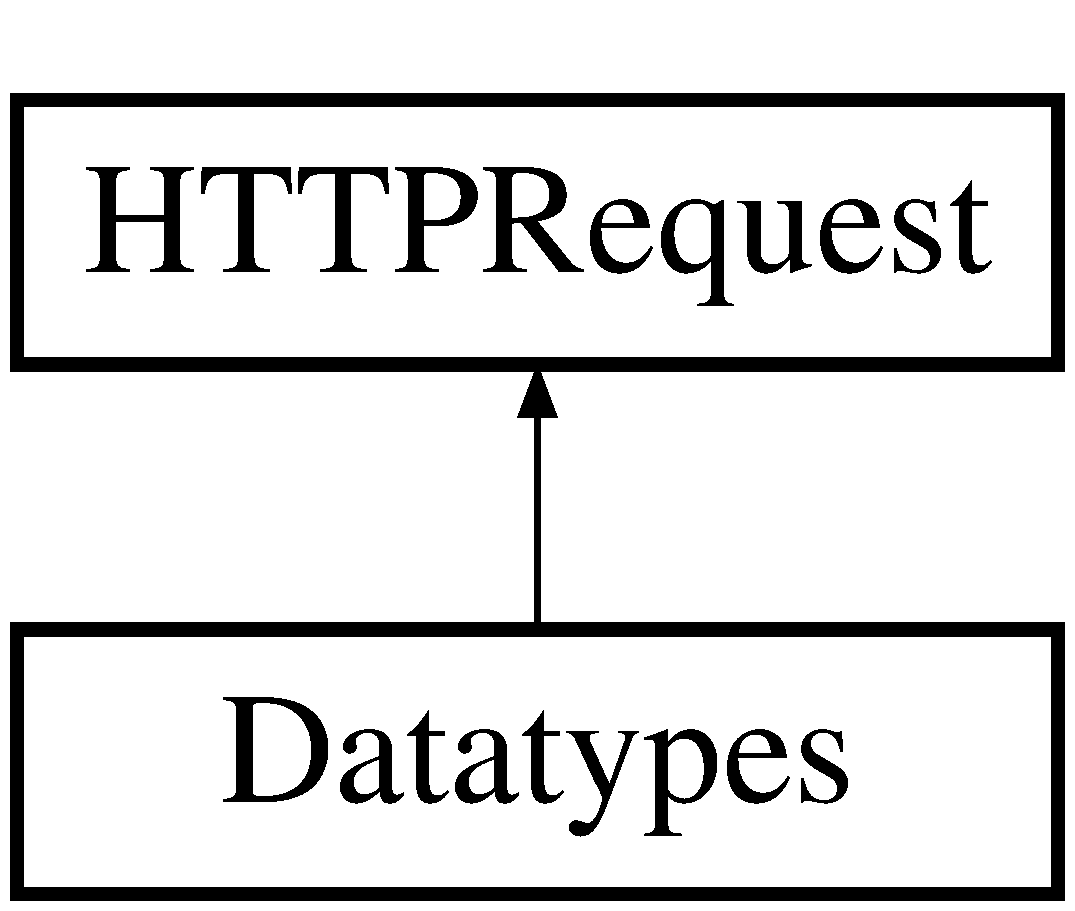
\includegraphics[height=2.000000cm]{classDatatypes}
\end{center}
\end{figure}
\subsection*{Public Member Functions}
\begin{DoxyCompactItemize}
\item 
\hyperlink{classDatatypes_a48b6d94f060f756ef7912b8bbdb8414c}{\+\_\+\+\_\+construct} (\$galaxy)
\item 
\hyperlink{classDatatypes_a720d7d878f95c3e8be5123ca994813a6}{sniffers} ()
\item 
\hyperlink{classDatatypes_acb539e0f93f2110b2455d319a19145b7}{converters} ()
\item 
\hyperlink{classDatatypes_a2db3d954fb3c4bda53cefcfff922677b}{edam\+Formats} ()
\item 
\hyperlink{classDatatypes_a0a0e9756ac8bec8717a14c774b6d5d35}{mapping} ()
\item 
\hyperlink{classDatatypes_a0cebf844acab0353ece6f1a5b2482935}{index} ()
\end{DoxyCompactItemize}
\subsection*{Additional Inherited Members}


\subsection{Constructor \& Destructor Documentation}
\index{Datatypes@{Datatypes}!\+\_\+\+\_\+construct@{\+\_\+\+\_\+construct}}
\index{\+\_\+\+\_\+construct@{\+\_\+\+\_\+construct}!Datatypes@{Datatypes}}
\subsubsection[{\texorpdfstring{\+\_\+\+\_\+construct(\$galaxy)}{\_\_construct($galaxy)}}]{\setlength{\rightskip}{0pt plus 5cm}Datatypes\+::\+\_\+\+\_\+construct (
\begin{DoxyParamCaption}
\item[{}]{\$galaxy}
\end{DoxyParamCaption}
)}\hypertarget{classDatatypes_a48b6d94f060f756ef7912b8bbdb8414c}{}\label{classDatatypes_a48b6d94f060f756ef7912b8bbdb8414c}
The Data\+Types constructor.


\begin{DoxyParams}[1]{Parameters}
\hyperlink{classGalaxyInstance}{Galaxy\+Instance} & {\em \$galaxy} & A \hyperlink{classGalaxyInstance}{Galaxy\+Instance} object.\\
\hline
\end{DoxyParams}
\begin{DoxyReturn}{Returns}
An instance of a \hyperlink{classDatatypes}{Datatypes} object. 
\end{DoxyReturn}


\subsection{Member Function Documentation}
\index{Datatypes@{Datatypes}!converters@{converters}}
\index{converters@{converters}!Datatypes@{Datatypes}}
\subsubsection[{\texorpdfstring{converters()}{converters()}}]{\setlength{\rightskip}{0pt plus 5cm}Datatypes\+::converters (
\begin{DoxyParamCaption}
{}
\end{DoxyParamCaption}
)}\hypertarget{classDatatypes_acb539e0f93f2110b2455d319a19145b7}{}\label{classDatatypes_acb539e0f93f2110b2455d319a19145b7}
Retreive a list of all datatype converters.

Corresponds to the Galaxy A\+P\+I/\+Path\+: G\+ET /api/datatypes/converters

\begin{DoxyReturn}{Returns}
An array containing converters of all datatypes 
\end{DoxyReturn}
\index{Datatypes@{Datatypes}!edam\+Formats@{edam\+Formats}}
\index{edam\+Formats@{edam\+Formats}!Datatypes@{Datatypes}}
\subsubsection[{\texorpdfstring{edam\+Formats()}{edamFormats()}}]{\setlength{\rightskip}{0pt plus 5cm}Datatypes\+::edam\+Formats (
\begin{DoxyParamCaption}
{}
\end{DoxyParamCaption}
)}\hypertarget{classDatatypes_a2db3d954fb3c4bda53cefcfff922677b}{}\label{classDatatypes_a2db3d954fb3c4bda53cefcfff922677b}
Retreive a list of all datatypes in the edam format.

Corresponds to the Galaxy A\+P\+I/\+Path\+: G\+ET /api/datatypes/edam\+\_\+formats

\begin{DoxyReturn}{Returns}
An array containing all datatypes in edam\+\_\+format. 
\end{DoxyReturn}
\index{Datatypes@{Datatypes}!index@{index}}
\index{index@{index}!Datatypes@{Datatypes}}
\subsubsection[{\texorpdfstring{index()}{index()}}]{\setlength{\rightskip}{0pt plus 5cm}Datatypes\+::index (
\begin{DoxyParamCaption}
{}
\end{DoxyParamCaption}
)}\hypertarget{classDatatypes_a0cebf844acab0353ece6f1a5b2482935}{}\label{classDatatypes_a0cebf844acab0353ece6f1a5b2482935}
Retreive a list of all datatypes

Corresponds to the Galaxy A\+P\+I/\+Path\+: G\+ET /api/datatypes/

\begin{DoxyReturn}{Returns}
An array containing all datatypes 
\end{DoxyReturn}
\index{Datatypes@{Datatypes}!mapping@{mapping}}
\index{mapping@{mapping}!Datatypes@{Datatypes}}
\subsubsection[{\texorpdfstring{mapping()}{mapping()}}]{\setlength{\rightskip}{0pt plus 5cm}Datatypes\+::mapping (
\begin{DoxyParamCaption}
{}
\end{DoxyParamCaption}
)}\hypertarget{classDatatypes_a0a0e9756ac8bec8717a14c774b6d5d35}{}\label{classDatatypes_a0a0e9756ac8bec8717a14c774b6d5d35}
Retreive a list of all datatypes in mapping.

Corresponds to the Galaxy A\+P\+I/\+Path\+: G\+ET /api/datatypes/mapping.

\begin{DoxyReturn}{Returns}
An array containing all datatypes in mapping. 
\end{DoxyReturn}
\index{Datatypes@{Datatypes}!sniffers@{sniffers}}
\index{sniffers@{sniffers}!Datatypes@{Datatypes}}
\subsubsection[{\texorpdfstring{sniffers()}{sniffers()}}]{\setlength{\rightskip}{0pt plus 5cm}Datatypes\+::sniffers (
\begin{DoxyParamCaption}
{}
\end{DoxyParamCaption}
)}\hypertarget{classDatatypes_a720d7d878f95c3e8be5123ca994813a6}{}\label{classDatatypes_a720d7d878f95c3e8be5123ca994813a6}
Retreive a list of all datatype sniffers.

Corresponds to the Galaxy A\+P\+I/\+Path\+: G\+ET /api/datatypes/sniffers

\begin{DoxyReturn}{Returns}
An array containing sniffers of all datatypes 
\end{DoxyReturn}


The documentation for this class was generated from the following file\+:\begin{DoxyCompactItemize}
\item 
\hyperlink{DataTypes_8inc}{Data\+Types.\+inc}\end{DoxyCompactItemize}

\hypertarget{classFolderContents}{}\section{Folder\+Contents Class Reference}
\label{classFolderContents}\index{Folder\+Contents@{Folder\+Contents}}
Inheritance diagram for Folder\+Contents\+:\begin{figure}[H]
\begin{center}
\leavevmode
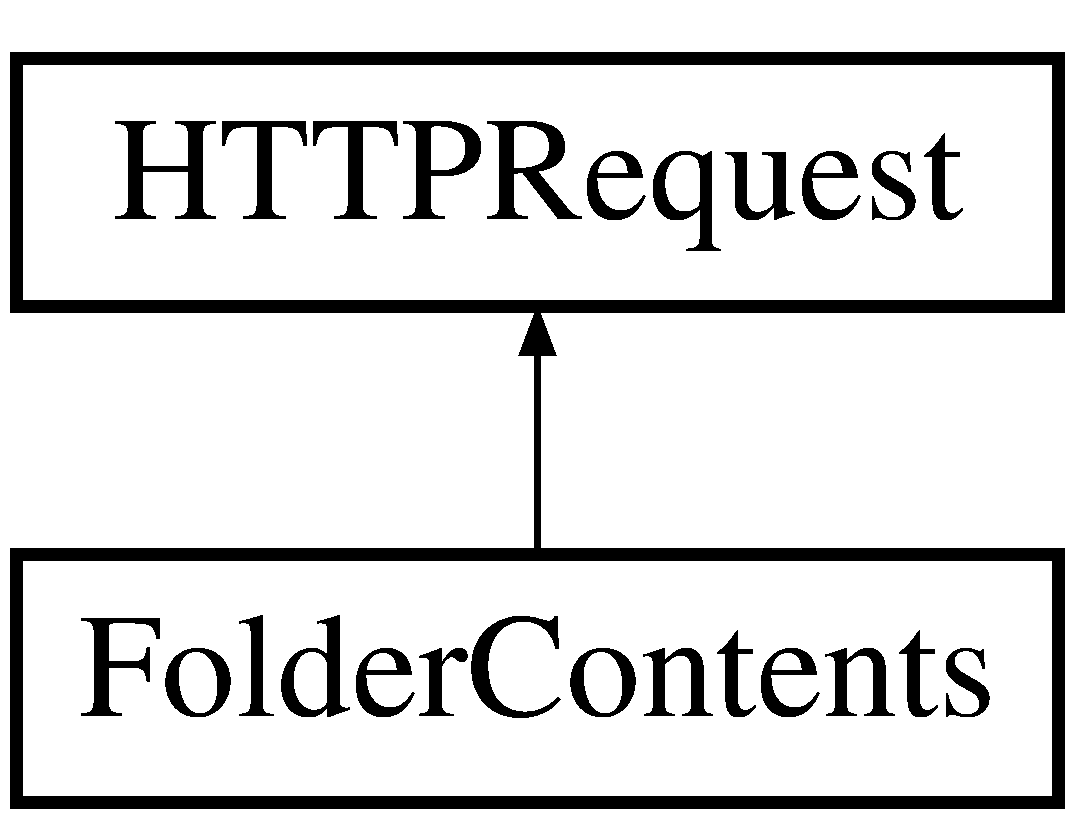
\includegraphics[height=2.000000cm]{classFolderContents}
\end{center}
\end{figure}
\subsection*{Public Member Functions}
\begin{DoxyCompactItemize}
\item 
\hyperlink{classFolderContents_a2d36ebf77aded6b7d8a07e963d8a86dd}{\+\_\+\+\_\+construct} (\$galaxy)
\item 
\hyperlink{classFolderContents_a3df4eff77c36fb37793595824fac74e4}{index} (\$folder\+\_\+id)
\item 
\hyperlink{classFolderContents_a3a74d968f4694357667bbdeed38a218f}{create} (\$parent\+\_\+folder\+\_\+id, \$from\+\_\+hda\+\_\+id=N\+U\+LL, \$ldda\+\_\+message=N\+U\+LL, \$extended\+\_\+metadata=N\+U\+LL)
\item 
\hyperlink{classFolderContents_a502b2757e6a8d148a858701f7a6ca2fd}{show} (\$folder\+\_\+id)
\item 
\hyperlink{classFolderContents_aca18be7b8009a751aa27b09702ae5997}{update} (\$folder\+\_\+id, \$add\+\_\+ids, \$manage\+\_\+ids, \$modify\+\_\+ids)
\end{DoxyCompactItemize}
\subsection*{Additional Inherited Members}


\subsection{Constructor \& Destructor Documentation}
\index{Folder\+Contents@{Folder\+Contents}!\+\_\+\+\_\+construct@{\+\_\+\+\_\+construct}}
\index{\+\_\+\+\_\+construct@{\+\_\+\+\_\+construct}!Folder\+Contents@{Folder\+Contents}}
\subsubsection[{\texorpdfstring{\+\_\+\+\_\+construct(\$galaxy)}{\_\_construct($galaxy)}}]{\setlength{\rightskip}{0pt plus 5cm}Folder\+Contents\+::\+\_\+\+\_\+construct (
\begin{DoxyParamCaption}
\item[{}]{\$galaxy}
\end{DoxyParamCaption}
)}\hypertarget{classFolderContents_a2d36ebf77aded6b7d8a07e963d8a86dd}{}\label{classFolderContents_a2d36ebf77aded6b7d8a07e963d8a86dd}
The \hyperlink{classFolderContents}{Folder\+Contents} constructor.


\begin{DoxyParams}[1]{Parameters}
\hyperlink{classGalaxyInstance}{Galaxy\+Instance} & {\em \$galaxy} & A \hyperlink{classGalaxyInstance}{Galaxy\+Instance} object.\\
\hline
\end{DoxyParams}
\begin{DoxyReturn}{Returns}
An instance of a \hyperlink{classFolderContents}{Folder\+Contents} object. 
\end{DoxyReturn}


\subsection{Member Function Documentation}
\index{Folder\+Contents@{Folder\+Contents}!create@{create}}
\index{create@{create}!Folder\+Contents@{Folder\+Contents}}
\subsubsection[{\texorpdfstring{create(\$parent\+\_\+folder\+\_\+id, \$from\+\_\+hda\+\_\+id=\+N\+U\+L\+L, \$ldda\+\_\+message=\+N\+U\+L\+L, \$extended\+\_\+metadata=\+N\+U\+L\+L)}{create($parent\_folder\_id, $from\_hda\_id=NULL, $ldda\_message=NULL, $extended\_metadata=NULL)}}]{\setlength{\rightskip}{0pt plus 5cm}Folder\+Contents\+::create (
\begin{DoxyParamCaption}
\item[{}]{\$parent\+\_\+folder\+\_\+id, }
\item[{}]{\$from\+\_\+hda\+\_\+id = {\ttfamily NULL}, }
\item[{}]{\$ldda\+\_\+message = {\ttfamily NULL}, }
\item[{}]{\$extended\+\_\+metadata = {\ttfamily NULL}}
\end{DoxyParamCaption}
)}\hypertarget{classFolderContents_a3a74d968f4694357667bbdeed38a218f}{}\label{classFolderContents_a3a74d968f4694357667bbdeed38a218f}
Create a new content for specified folder

Corresponds to the Galaxy A\+P\+I/path at\+: P\+O\+ST /api/folders/\{folder\+\_\+id\}/contents


\begin{DoxyParams}{Parameters}
{\em \$parent\+\_\+folder\+\_\+id} & The parent folder of the new item To obtain id, see the \hyperlink{classFolderContents_a3df4eff77c36fb37793595824fac74e4}{index()} function in the Folder class. \\
\hline
{\em \$from\+\_\+hda\+\_\+id} & (optional) The id of an accessible H\+DA to into the library To obtain this id, see \hyperlink{classFolderContents_a3df4eff77c36fb37793595824fac74e4}{index()} in \hyperlink{classHistoryContents}{History\+Contents} class. \\
\hline
{\em \$ldda\+\_\+messge} & (optional) Any message to send along with the Library\+Dataset\+Dataset\+Association. \\
\hline
{\em \$extented\+\_\+metadata} & (optional) Sub-\/dictionary containing any extended metadata to associate with the item.\\
\hline
\end{DoxyParams}
\begin{DoxyReturn}{Returns}
An array containing the newly created folder content. 
\end{DoxyReturn}
\index{Folder\+Contents@{Folder\+Contents}!index@{index}}
\index{index@{index}!Folder\+Contents@{Folder\+Contents}}
\subsubsection[{\texorpdfstring{index(\$folder\+\_\+id)}{index($folder\_id)}}]{\setlength{\rightskip}{0pt plus 5cm}Folder\+Contents\+::index (
\begin{DoxyParamCaption}
\item[{}]{\$folder\+\_\+id}
\end{DoxyParamCaption}
)}\hypertarget{classFolderContents_a3df4eff77c36fb37793595824fac74e4}{}\label{classFolderContents_a3df4eff77c36fb37793595824fac74e4}
Displays all the contents of a folder.

Corresponds to the Galaxy A\+P\+I/path\+: G\+ET /api/folders/F\{folder\+\_\+id\}/contents.


\begin{DoxyParams}{Parameters}
{\em \$folder\+\_\+id} & Id of the folder whos contents to display. To obtain id, see the \hyperlink{classFolderContents_a3df4eff77c36fb37793595824fac74e4}{index()} function in the Folder class. \\
\hline
\end{DoxyParams}
\begin{DoxyReturn}{Returns}
An array of The specified folder\textquotesingle{}s contents 
\end{DoxyReturn}
\index{Folder\+Contents@{Folder\+Contents}!show@{show}}
\index{show@{show}!Folder\+Contents@{Folder\+Contents}}
\subsubsection[{\texorpdfstring{show(\$folder\+\_\+id)}{show($folder\_id)}}]{\setlength{\rightskip}{0pt plus 5cm}Folder\+Contents\+::show (
\begin{DoxyParamCaption}
\item[{}]{\$folder\+\_\+id}
\end{DoxyParamCaption}
)}\hypertarget{classFolderContents_a502b2757e6a8d148a858701f7a6ca2fd}{}\label{classFolderContents_a502b2757e6a8d148a858701f7a6ca2fd}
Retreive details of for a specified folder.

Corresponds to the Galaxy A\+P\+I/path\+: G\+ET /api/folders/\{folder\+\_\+id\}/


\begin{DoxyParams}{Parameters}
{\em \$folder\+\_\+id} & The id of the folder to view\\
\hline
\end{DoxyParams}
\begin{DoxyReturn}{Returns}
False. 
\end{DoxyReturn}
\index{Folder\+Contents@{Folder\+Contents}!update@{update}}
\index{update@{update}!Folder\+Contents@{Folder\+Contents}}
\subsubsection[{\texorpdfstring{update(\$folder\+\_\+id, \$add\+\_\+ids, \$manage\+\_\+ids, \$modify\+\_\+ids)}{update($folder\_id, $add\_ids, $manage\_ids, $modify\_ids)}}]{\setlength{\rightskip}{0pt plus 5cm}Folder\+Contents\+::update (
\begin{DoxyParamCaption}
\item[{}]{\$folder\+\_\+id, }
\item[{}]{\$add\+\_\+ids, }
\item[{}]{\$manage\+\_\+ids, }
\item[{}]{\$modify\+\_\+ids}
\end{DoxyParamCaption}
)}\hypertarget{classFolderContents_aca18be7b8009a751aa27b09702ae5997}{}\label{classFolderContents_aca18be7b8009a751aa27b09702ae5997}
Update the contents to a specific folder

Corresponds to the Galaxy A\+P\+I/\+P\+A\+TH P\+UT /api/folders/\{folder\+\_\+id\}/

\begin{DoxyReturn}{Returns}
False. 
\end{DoxyReturn}


The documentation for this class was generated from the following file\+:\begin{DoxyCompactItemize}
\item 
\hyperlink{FolderContents_8inc}{Folder\+Contents.\+inc}\end{DoxyCompactItemize}

\hypertarget{classFolders}{}\section{Folders Class Reference}
\label{classFolders}\index{Folders@{Folders}}
Inheritance diagram for Folders\+:\begin{figure}[H]
\begin{center}
\leavevmode
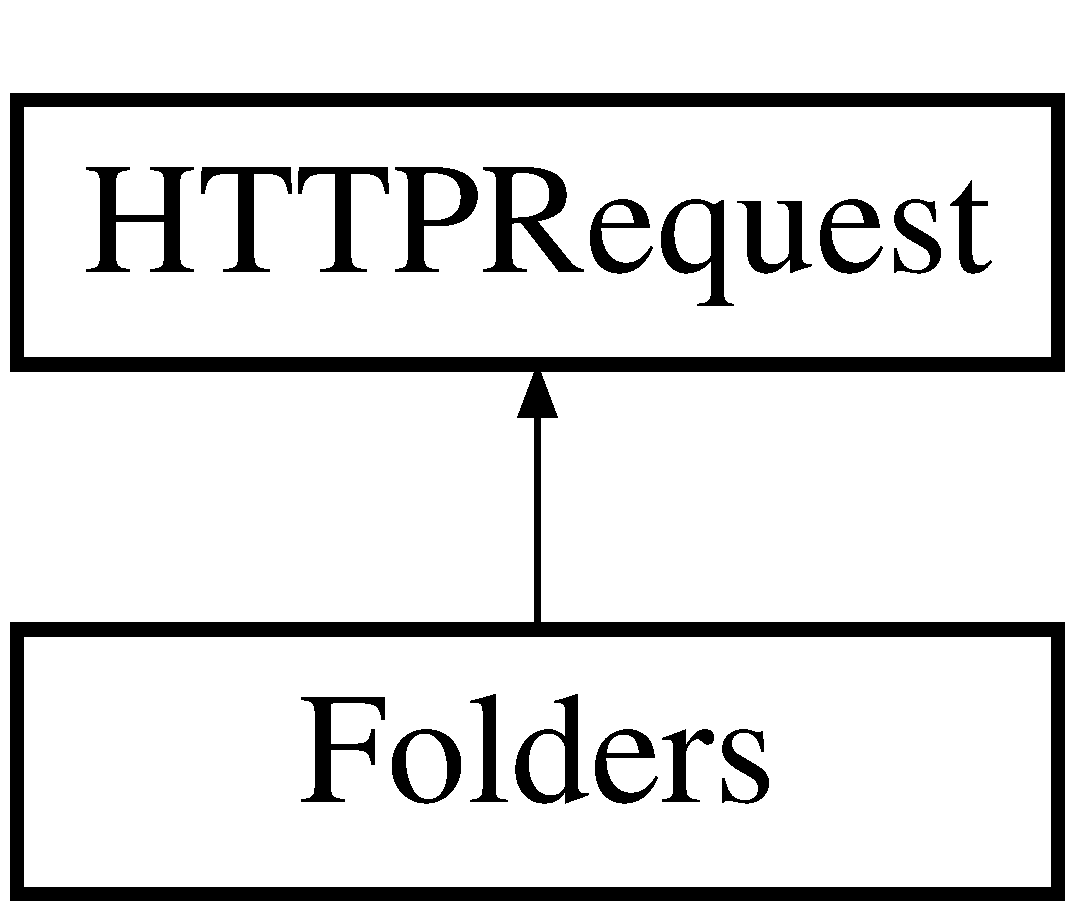
\includegraphics[height=2.000000cm]{classFolders}
\end{center}
\end{figure}
\subsection*{Public Member Functions}
\begin{DoxyCompactItemize}
\item 
\hyperlink{classFolders_a47219b896724ee4ac920d05cd87acf7d}{\+\_\+\+\_\+construct} (\$galaxy)
\item 
\hyperlink{classFolders_a109d9c4a860921d86ee2b892172c4cb7}{index} ()
\item 
\hyperlink{classFolders_a7ec1832769976e6192b010e8c93bdcea}{show} (\$folder\+\_\+id)
\item 
\hyperlink{classFolders_aee151f1b40f0a3ae61afb943469e5339}{create} (\$parent\+\_\+folder\+\_\+id, \$name, \$description)
\item 
\hyperlink{classFolders_a68817a94c13feb8112e4d518ca1f9b7d}{get\+Permissions} (\$folder\+\_\+id)
\item 
\hyperlink{classFolders_ab367992f8589996cf357d389045f06d5}{set\+Permissions} (\$folder\+\_\+id, \$add\+\_\+ids, \$manage\+\_\+ids, \$modify\+\_\+ids)
\item 
\hyperlink{classFolders_ae0ad5e1d1020ecd6542fe01c1dd4c573}{delete} (\$folder\+\_\+id, \$undelete=F\+A\+L\+SE)
\item 
\hyperlink{classFolders_aef4ad6a8938fbf0144d147169952a4c1}{update} (\$folder\+\_\+id, \$payload)
\end{DoxyCompactItemize}
\subsection*{Additional Inherited Members}


\subsection{Constructor \& Destructor Documentation}
\index{Folders@{Folders}!\+\_\+\+\_\+construct@{\+\_\+\+\_\+construct}}
\index{\+\_\+\+\_\+construct@{\+\_\+\+\_\+construct}!Folders@{Folders}}
\subsubsection[{\texorpdfstring{\+\_\+\+\_\+construct(\$galaxy)}{\_\_construct($galaxy)}}]{\setlength{\rightskip}{0pt plus 5cm}Folders\+::\+\_\+\+\_\+construct (
\begin{DoxyParamCaption}
\item[{}]{\$galaxy}
\end{DoxyParamCaption}
)}\hypertarget{classFolders_a47219b896724ee4ac920d05cd87acf7d}{}\label{classFolders_a47219b896724ee4ac920d05cd87acf7d}
The \hyperlink{classFolders}{Folders} constructor.


\begin{DoxyParams}[1]{Parameters}
\hyperlink{classGalaxyInstance}{Galaxy\+Instance} & {\em \$galaxy} & A \hyperlink{classGalaxyInstance}{Galaxy\+Instance} object.\\
\hline
\end{DoxyParams}
\begin{DoxyReturn}{Returns}
An instance of a \hyperlink{classFolders}{Folders} object. 
\end{DoxyReturn}


\subsection{Member Function Documentation}
\index{Folders@{Folders}!create@{create}}
\index{create@{create}!Folders@{Folders}}
\subsubsection[{\texorpdfstring{create(\$parent\+\_\+folder\+\_\+id, \$name, \$description)}{create($parent\_folder\_id, $name, $description)}}]{\setlength{\rightskip}{0pt plus 5cm}Folders\+::create (
\begin{DoxyParamCaption}
\item[{}]{\$parent\+\_\+folder\+\_\+id, }
\item[{}]{\$name, }
\item[{}]{\$description}
\end{DoxyParamCaption}
)}\hypertarget{classFolders_aee151f1b40f0a3ae61afb943469e5339}{}\label{classFolders_aee151f1b40f0a3ae61afb943469e5339}
Create a new folder.

Corresponds to the A\+PI function/path\+: P\+O\+ST /api/folders/\{encoded\+\_\+parent\+\_\+folder\+\_\+id\}


\begin{DoxyParams}{Parameters}
{\em \$parent\+\_\+folder\+\_\+id} & The id of the parent folder that this folder will be created under. \\
\hline
{\em \$name} & The name of your new folder. \\
\hline
{\em \$description} & The description of your new folder.\\
\hline
\end{DoxyParams}
\begin{DoxyReturn}{Returns}
An array containing information on the new folder. 
\end{DoxyReturn}
\index{Folders@{Folders}!delete@{delete}}
\index{delete@{delete}!Folders@{Folders}}
\subsubsection[{\texorpdfstring{delete(\$folder\+\_\+id, \$undelete=\+F\+A\+L\+S\+E)}{delete($folder\_id, $undelete=FALSE)}}]{\setlength{\rightskip}{0pt plus 5cm}Folders\+::delete (
\begin{DoxyParamCaption}
\item[{}]{\$folder\+\_\+id, }
\item[{}]{\$undelete = {\ttfamily FALSE}}
\end{DoxyParamCaption}
)}\hypertarget{classFolders_ae0ad5e1d1020ecd6542fe01c1dd4c573}{}\label{classFolders_ae0ad5e1d1020ecd6542fe01c1dd4c573}
Mark the folder as \textquotesingle{}deleted\textquotesingle{} or \textquotesingle{}undeleted\textquotesingle{}.

Corresponds to the Galaxy A\+PI function at D\+E\+L\+E\+TE /api/folders/\{folder\+\_\+id\}/

Only admin users can delete/undelete folders


\begin{DoxyParams}{Parameters}
{\em \$folder\+\_\+id} & The folder you want to delete/undelete. To obtain a folder id, please use this class\textquotesingle{}s \hyperlink{classFolders_a109d9c4a860921d86ee2b892172c4cb7}{index()} function. \\
\hline
{\em \$undelete} & Specifying whether the item should be deleted(true) or undeleted (false).\\
\hline
\end{DoxyParams}
\begin{DoxyReturn}{Returns}
Json Array containing information on the deleted (or undeleted) folder. 
\end{DoxyReturn}
\index{Folders@{Folders}!get\+Permissions@{get\+Permissions}}
\index{get\+Permissions@{get\+Permissions}!Folders@{Folders}}
\subsubsection[{\texorpdfstring{get\+Permissions(\$folder\+\_\+id)}{getPermissions($folder\_id)}}]{\setlength{\rightskip}{0pt plus 5cm}Folders\+::get\+Permissions (
\begin{DoxyParamCaption}
\item[{}]{\$folder\+\_\+id}
\end{DoxyParamCaption}
)}\hypertarget{classFolders_a68817a94c13feb8112e4d518ca1f9b7d}{}\label{classFolders_a68817a94c13feb8112e4d518ca1f9b7d}
Load all permissions for the folder with the given id.

Corresponds to the Galaxy A\+P\+I/\+Path\+: G\+ET /api/folders/\{folder\+\_\+id\}/permissions


\begin{DoxyParams}{Parameters}
{\em \$folder\+\_\+id} & The id of the folder to view permissions. The id can be ontained using the \hyperlink{classFolders_a109d9c4a860921d86ee2b892172c4cb7}{index()} function in this class.\\
\hline
\end{DoxyParams}
\begin{DoxyReturn}{Returns}
An array containing permission information on a specified folder. 
\end{DoxyReturn}
\index{Folders@{Folders}!index@{index}}
\index{index@{index}!Folders@{Folders}}
\subsubsection[{\texorpdfstring{index()}{index()}}]{\setlength{\rightskip}{0pt plus 5cm}Folders\+::index (
\begin{DoxyParamCaption}
{}
\end{DoxyParamCaption}
)}\hypertarget{classFolders_a109d9c4a860921d86ee2b892172c4cb7}{}\label{classFolders_a109d9c4a860921d86ee2b892172c4cb7}
Retreive information about folders.

Corresponds to the Galaxy A\+PI function/path\+: G\+ET /api/folders/

\begin{DoxyReturn}{Returns}
An array containing information about the specified folder. 
\end{DoxyReturn}
\index{Folders@{Folders}!set\+Permissions@{set\+Permissions}}
\index{set\+Permissions@{set\+Permissions}!Folders@{Folders}}
\subsubsection[{\texorpdfstring{set\+Permissions(\$folder\+\_\+id, \$add\+\_\+ids, \$manage\+\_\+ids, \$modify\+\_\+ids)}{setPermissions($folder\_id, $add\_ids, $manage\_ids, $modify\_ids)}}]{\setlength{\rightskip}{0pt plus 5cm}Folders\+::set\+Permissions (
\begin{DoxyParamCaption}
\item[{}]{\$folder\+\_\+id, }
\item[{}]{\$add\+\_\+ids, }
\item[{}]{\$manage\+\_\+ids, }
\item[{}]{\$modify\+\_\+ids}
\end{DoxyParamCaption}
)}\hypertarget{classFolders_ab367992f8589996cf357d389045f06d5}{}\label{classFolders_ab367992f8589996cf357d389045f06d5}
Set permissions for a specified folder.

Corresponds to the Galaxy A\+PI function/path at\+: P\+O\+ST /api/folders/\{folder\+\_\+id\}/permissions There are 3 options that can be manipulated\+:
\begin{DoxyEnumerate}
\item Modify library item\+: \hyperlink{classUsers}{Users} can modify this library (\$folder\+\_\+id) item
\item Add library item\+: \hyperlink{classUsers}{Users} can add library items to this (\$folder\+\_\+id) item
\item Manage library permissions\+: \hyperlink{classUsers}{Users} can manage roles associated with permissions on this library item
\end{DoxyEnumerate}


\begin{DoxyParams}{Parameters}
{\em \$folder\+\_\+id} & The folder you want to view permissions. To obtain a folder id, please use the \hyperlink{classFolders_a109d9c4a860921d86ee2b892172c4cb7}{index()} function in this class. \\
\hline
{\em \$add\+\_\+ids} & List of users that will have add item permission on the folder. To obtain a user id, please use the user class\textquotesingle{}s \hyperlink{classFolders_a109d9c4a860921d86ee2b892172c4cb7}{index()} function. \\
\hline
{\em \$manage\+\_\+ids} & List of users that will have manage permission on the folder \\
\hline
{\em \$modify\+\_\+ids} & An array of users that will have modify permission on the folder \\
\hline
\end{DoxyParams}
\index{Folders@{Folders}!show@{show}}
\index{show@{show}!Folders@{Folders}}
\subsubsection[{\texorpdfstring{show(\$folder\+\_\+id)}{show($folder\_id)}}]{\setlength{\rightskip}{0pt plus 5cm}Folders\+::show (
\begin{DoxyParamCaption}
\item[{}]{\$folder\+\_\+id}
\end{DoxyParamCaption}
)}\hypertarget{classFolders_a7ec1832769976e6192b010e8c93bdcea}{}\label{classFolders_a7ec1832769976e6192b010e8c93bdcea}
Retreive information about a specific folder

Corresponds to the Galaxy A\+PI function/path\+: G\+ET /api/folders/\{folder\+\_\+id\}


\begin{DoxyParams}{Parameters}
{\em \$folder\+\_\+id} & The folder that you would like to see. Please see the \hyperlink{classFolders_a109d9c4a860921d86ee2b892172c4cb7}{index()} function in this class to obtain folder ids.\\
\hline
\end{DoxyParams}
\begin{DoxyReturn}{Returns}
An array containing information about the specified folder. 
\end{DoxyReturn}
\index{Folders@{Folders}!update@{update}}
\index{update@{update}!Folders@{Folders}}
\subsubsection[{\texorpdfstring{update(\$folder\+\_\+id, \$payload)}{update($folder\_id, $payload)}}]{\setlength{\rightskip}{0pt plus 5cm}Folders\+::update (
\begin{DoxyParamCaption}
\item[{}]{\$folder\+\_\+id, }
\item[{}]{\$payload}
\end{DoxyParamCaption}
)}\hypertarget{classFolders_aef4ad6a8938fbf0144d147169952a4c1}{}\label{classFolders_aef4ad6a8938fbf0144d147169952a4c1}
Updated the folder\textquotesingle{}s name and description.

Corresponds to the Galaxy A\+P\+I/path at\+: P\+A\+T\+CH /api/folders/\{folder\+\_\+id\}/

Only admin users can update folders.


\begin{DoxyParams}{Parameters}
{\em \$folder\+\_\+id} & The folder you want to update \\
\hline
{\em \$payload} & An array that contains \textquotesingle{}name\textquotesingle{} =$>$ \mbox{[}new\+\_\+name\mbox{]} and \textquotesingle{}description\textquotesingle{} =$>$ \mbox{[}can be null\mbox{]}.\\
\hline
\end{DoxyParams}
\begin{DoxyReturn}{Returns}
Json array containing details about the deleted file history content. 
\end{DoxyReturn}


The documentation for this class was generated from the following file\+:\begin{DoxyCompactItemize}
\item 
\hyperlink{Folders_8inc}{Folders.\+inc}\end{DoxyCompactItemize}

\hypertarget{classGalaxyInstance}{\section{Galaxy\-Instance Class Reference}
\label{classGalaxyInstance}\index{Galaxy\-Instance@{Galaxy\-Instance}}
}
Inheritance diagram for Galaxy\-Instance\-:\begin{figure}[H]
\begin{center}
\leavevmode
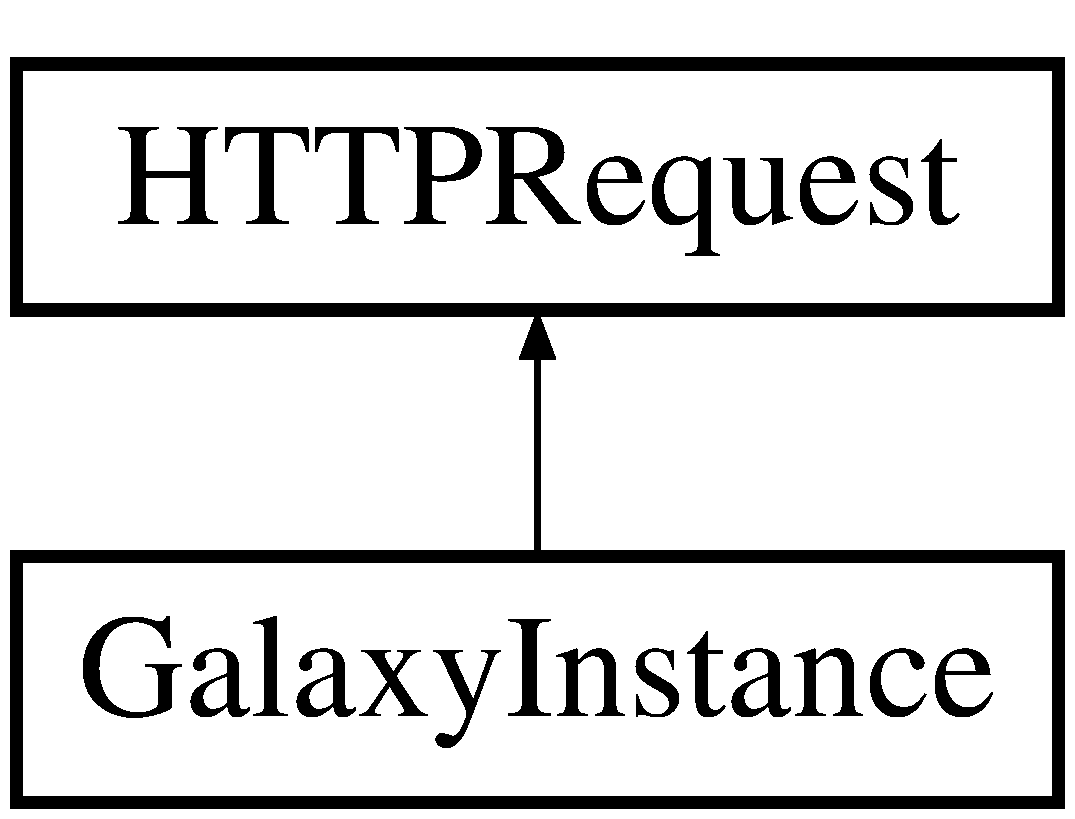
\includegraphics[height=2.000000cm]{classGalaxyInstance}
\end{center}
\end{figure}
\subsection*{Public Member Functions}
\begin{DoxyCompactItemize}
\item 
\hyperlink{classGalaxyInstance_a98d1b5f750ce3be53e96e435917b63b1}{\-\_\-\-\_\-construct} (\$hostname, \$port, \$use\-\_\-https=F\-A\-L\-S\-E)
\item 
\hyperlink{classGalaxyInstance_afbb7256306223f7f8ee85f85868e2de2}{get\-Version} ()
\item 
\hyperlink{classGalaxyInstance_a243315a49fd4ba0df8916b87872299ed}{authenticate} (\$username, \$password, \&\$message= '')
\item 
\hyperlink{classGalaxyInstance_a5b0c7191b82c21d857ec3d42068f3cf4}{get\-U\-R\-L} ()
\item 
\hyperlink{classGalaxyInstance_a4e4c854e91c21917adebec78a655edd3}{set\-A\-P\-I\-Key} (\$api\-\_\-key)
\item 
\hyperlink{classGalaxyInstance_a563deeb4f829462d7476d3684ed099cb}{get\-A\-P\-I\-Key} ()
\end{DoxyCompactItemize}
\subsection*{Protected Attributes}
\begin{DoxyCompactItemize}
\item 
\hyperlink{classGalaxyInstance_a68aaf747e0eae3b9338cd4c51711b514}{\$host}
\item 
\hyperlink{classGalaxyInstance_ab70c08b0781f835e1a2e4388b1baa639}{\$port}
\item 
\hyperlink{classGalaxyInstance_ab920cbfc8f2f63f3793ba067ee523ca8}{\$use\-\_\-https}
\item 
\hyperlink{classGalaxyInstance_a2a67b0838ca6175e9e01e3045b666caf}{\$api\-\_\-key}
\end{DoxyCompactItemize}


\subsection{Constructor \& Destructor Documentation}
\hypertarget{classGalaxyInstance_a98d1b5f750ce3be53e96e435917b63b1}{\index{Galaxy\-Instance@{Galaxy\-Instance}!\-\_\-\-\_\-construct@{\-\_\-\-\_\-construct}}
\index{\-\_\-\-\_\-construct@{\-\_\-\-\_\-construct}!GalaxyInstance@{Galaxy\-Instance}}
\subsubsection[{\-\_\-\-\_\-construct}]{\setlength{\rightskip}{0pt plus 5cm}Galaxy\-Instance\-::\-\_\-\-\_\-construct (
\begin{DoxyParamCaption}
\item[{}]{\$hostname, }
\item[{}]{\$port, }
\item[{}]{\$use\-\_\-https = {\ttfamily FALSE}}
\end{DoxyParamCaption}
)}}\label{classGalaxyInstance_a98d1b5f750ce3be53e96e435917b63b1}
The \hyperlink{classGalaxyInstance}{Galaxy\-Instance} constructor.


\begin{DoxyParams}{Parameters}
{\em \$hostname} & The hostname where the Galaxy server is located. \\
\hline
{\em \$port} & The port on which the remote Galaxy instance is runinng. \\
\hline
{\em \$use\-\_\-https} & Should be set to T\-R\-U\-E if the remote server uses H\-T\-T\-P\-S. Defaults to T\-R\-U\-E.\\
\hline
\end{DoxyParams}
\begin{DoxyReturn}{Returns}
An instance of a \hyperlink{classGalaxyInstance}{Galaxy\-Instance} object. 
\end{DoxyReturn}


\subsection{Member Function Documentation}
\hypertarget{classGalaxyInstance_a243315a49fd4ba0df8916b87872299ed}{\index{Galaxy\-Instance@{Galaxy\-Instance}!authenticate@{authenticate}}
\index{authenticate@{authenticate}!GalaxyInstance@{Galaxy\-Instance}}
\subsubsection[{authenticate}]{\setlength{\rightskip}{0pt plus 5cm}Galaxy\-Instance\-::authenticate (
\begin{DoxyParamCaption}
\item[{}]{\$username, }
\item[{}]{\$password, }
\item[{\&}]{\$message = {\ttfamily ''}}
\end{DoxyParamCaption}
)}}\label{classGalaxyInstance_a243315a49fd4ba0df8916b87872299ed}
Authenticates a user with the remote Galaxy instance.

Corresponds to the Galaxy A\-P\-I method and path\-: G\-E\-T /api/authenticate/baseauth


\begin{DoxyParams}{Parameters}
{\em \$username} & The username of the user. \\
\hline
{\em \$password} & The password for the user. \\
\hline
{\em \$message} & If authentication fails then this variable will be set to contain the error message.\\
\hline
\end{DoxyParams}
\begin{DoxyReturn}{Returns}
T\-R\-U\-E if authentication was successful, F\-A\-L\-S\-E otherwise. 
\end{DoxyReturn}
\hypertarget{classGalaxyInstance_a563deeb4f829462d7476d3684ed099cb}{\index{Galaxy\-Instance@{Galaxy\-Instance}!get\-A\-P\-I\-Key@{get\-A\-P\-I\-Key}}
\index{get\-A\-P\-I\-Key@{get\-A\-P\-I\-Key}!GalaxyInstance@{Galaxy\-Instance}}
\subsubsection[{get\-A\-P\-I\-Key}]{\setlength{\rightskip}{0pt plus 5cm}Galaxy\-Instance\-::get\-A\-P\-I\-Key (
\begin{DoxyParamCaption}
{}
\end{DoxyParamCaption}
)}}\label{classGalaxyInstance_a563deeb4f829462d7476d3684ed099cb}
Acquires the A\-P\-I key

\begin{DoxyReturn}{Returns}
string The A\-P\-I key that authorizes a user to certain actions. 
\end{DoxyReturn}
\hypertarget{classGalaxyInstance_a5b0c7191b82c21d857ec3d42068f3cf4}{\index{Galaxy\-Instance@{Galaxy\-Instance}!get\-U\-R\-L@{get\-U\-R\-L}}
\index{get\-U\-R\-L@{get\-U\-R\-L}!GalaxyInstance@{Galaxy\-Instance}}
\subsubsection[{get\-U\-R\-L}]{\setlength{\rightskip}{0pt plus 5cm}Galaxy\-Instance\-::get\-U\-R\-L (
\begin{DoxyParamCaption}
{}
\end{DoxyParamCaption}
)}}\label{classGalaxyInstance_a5b0c7191b82c21d857ec3d42068f3cf4}
Returns the U\-R\-L for the remote Galaxy server.

The U\-R\-L returned will include the protocol (H\-T\-T\-P, H\-T\-T\-P\-S), the hostname and the port.

\begin{DoxyReturn}{Returns}
string The U\-R\-L for the remote Galaxy instance. 
\end{DoxyReturn}
\hypertarget{classGalaxyInstance_afbb7256306223f7f8ee85f85868e2de2}{\index{Galaxy\-Instance@{Galaxy\-Instance}!get\-Version@{get\-Version}}
\index{get\-Version@{get\-Version}!GalaxyInstance@{Galaxy\-Instance}}
\subsubsection[{get\-Version}]{\setlength{\rightskip}{0pt plus 5cm}Galaxy\-Instance\-::get\-Version (
\begin{DoxyParamCaption}
{}
\end{DoxyParamCaption}
)}}\label{classGalaxyInstance_afbb7256306223f7f8ee85f85868e2de2}
Retrieves the version of the Galaxy A\-P\-I.

\begin{DoxyReturn}{Returns}

\end{DoxyReturn}
\hypertarget{classGalaxyInstance_a4e4c854e91c21917adebec78a655edd3}{\index{Galaxy\-Instance@{Galaxy\-Instance}!set\-A\-P\-I\-Key@{set\-A\-P\-I\-Key}}
\index{set\-A\-P\-I\-Key@{set\-A\-P\-I\-Key}!GalaxyInstance@{Galaxy\-Instance}}
\subsubsection[{set\-A\-P\-I\-Key}]{\setlength{\rightskip}{0pt plus 5cm}Galaxy\-Instance\-::set\-A\-P\-I\-Key (
\begin{DoxyParamCaption}
\item[{}]{\$api\-\_\-key}
\end{DoxyParamCaption}
)}}\label{classGalaxyInstance_a4e4c854e91c21917adebec78a655edd3}
Sets the A\-P\-I Key for this Galaxy instance.


\begin{DoxyParams}{Parameters}
{\em \$api\-\_\-key} & The A\-P\-I key of the Galaxy user. \\
\hline
\end{DoxyParams}


\subsection{Member Data Documentation}
\hypertarget{classGalaxyInstance_a2a67b0838ca6175e9e01e3045b666caf}{\index{Galaxy\-Instance@{Galaxy\-Instance}!\$api\-\_\-key@{\$api\-\_\-key}}
\index{\$api\-\_\-key@{\$api\-\_\-key}!GalaxyInstance@{Galaxy\-Instance}}
\subsubsection[{\$api\-\_\-key}]{\setlength{\rightskip}{0pt plus 5cm}Galaxy\-Instance\-::\$api\-\_\-key\hspace{0.3cm}{\ttfamily [protected]}}}\label{classGalaxyInstance_a2a67b0838ca6175e9e01e3045b666caf}
The A\-P\-I Key for the user connection. \hypertarget{classGalaxyInstance_a68aaf747e0eae3b9338cd4c51711b514}{\index{Galaxy\-Instance@{Galaxy\-Instance}!\$host@{\$host}}
\index{\$host@{\$host}!GalaxyInstance@{Galaxy\-Instance}}
\subsubsection[{\$host}]{\setlength{\rightskip}{0pt plus 5cm}Galaxy\-Instance\-::\$host\hspace{0.3cm}{\ttfamily [protected]}}}\label{classGalaxyInstance_a68aaf747e0eae3b9338cd4c51711b514}
The hostname where the Galaxy server is located. \hypertarget{classGalaxyInstance_ab70c08b0781f835e1a2e4388b1baa639}{\index{Galaxy\-Instance@{Galaxy\-Instance}!\$port@{\$port}}
\index{\$port@{\$port}!GalaxyInstance@{Galaxy\-Instance}}
\subsubsection[{\$port}]{\setlength{\rightskip}{0pt plus 5cm}Galaxy\-Instance\-::\$port\hspace{0.3cm}{\ttfamily [protected]}}}\label{classGalaxyInstance_ab70c08b0781f835e1a2e4388b1baa639}
The port on which the remote Galaxy instance is runinng. \hypertarget{classGalaxyInstance_ab920cbfc8f2f63f3793ba067ee523ca8}{\index{Galaxy\-Instance@{Galaxy\-Instance}!\$use\-\_\-https@{\$use\-\_\-https}}
\index{\$use\-\_\-https@{\$use\-\_\-https}!GalaxyInstance@{Galaxy\-Instance}}
\subsubsection[{\$use\-\_\-https}]{\setlength{\rightskip}{0pt plus 5cm}Galaxy\-Instance\-::\$use\-\_\-https\hspace{0.3cm}{\ttfamily [protected]}}}\label{classGalaxyInstance_ab920cbfc8f2f63f3793ba067ee523ca8}
Should be set to T\-R\-U\-E if the remote server uses H\-T\-T\-P\-S. 

The documentation for this class was generated from the following file\-:\begin{DoxyCompactItemize}
\item 
Galaxy\-Instance.\-inc\end{DoxyCompactItemize}

\hypertarget{classGenomes}{}\section{Genomes Class Reference}
\label{classGenomes}\index{Genomes@{Genomes}}
Inheritance diagram for Genomes\+:\begin{figure}[H]
\begin{center}
\leavevmode
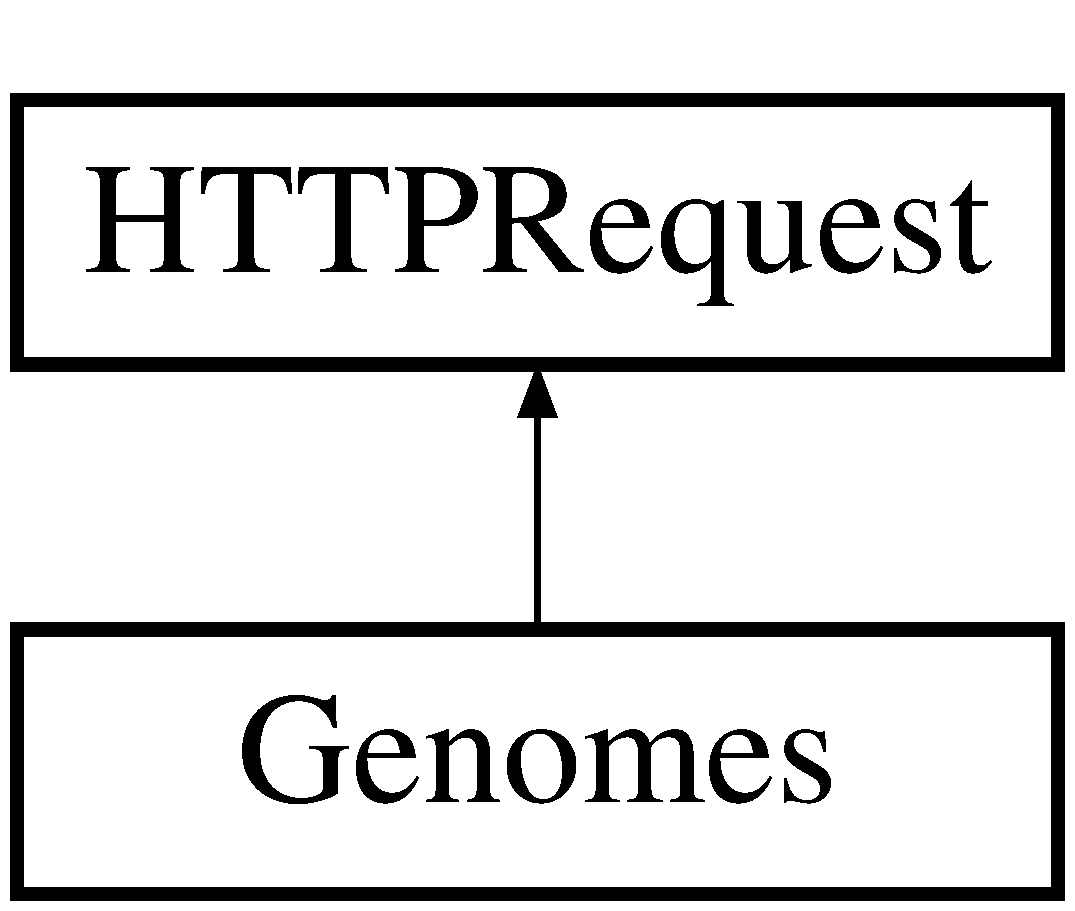
\includegraphics[height=2.000000cm]{classGenomes}
\end{center}
\end{figure}
\subsection*{Public Member Functions}
\begin{DoxyCompactItemize}
\item 
\hyperlink{classGenomes_a5c2d3df343e100b44466b7b81c9fda92}{\+\_\+\+\_\+construct} (\$galaxy)
\item 
\hyperlink{classGenomes_a52b51e90995539b8defb2571edd14437}{index} ()
\item 
\hyperlink{classGenomes_a44a6fccdb31050f3d4eae4143482355c}{show} (\$genome\+\_\+id)
\end{DoxyCompactItemize}
\subsection*{Additional Inherited Members}


\subsection{Constructor \& Destructor Documentation}
\index{Genomes@{Genomes}!\+\_\+\+\_\+construct@{\+\_\+\+\_\+construct}}
\index{\+\_\+\+\_\+construct@{\+\_\+\+\_\+construct}!Genomes@{Genomes}}
\subsubsection[{\texorpdfstring{\+\_\+\+\_\+construct(\$galaxy)}{\_\_construct($galaxy)}}]{\setlength{\rightskip}{0pt plus 5cm}Genomes\+::\+\_\+\+\_\+construct (
\begin{DoxyParamCaption}
\item[{}]{\$galaxy}
\end{DoxyParamCaption}
)}\hypertarget{classGenomes_a5c2d3df343e100b44466b7b81c9fda92}{}\label{classGenomes_a5c2d3df343e100b44466b7b81c9fda92}
The \hyperlink{classGenomes}{Genomes} constructor.


\begin{DoxyParams}[1]{Parameters}
\hyperlink{classGalaxyInstance}{Galaxy\+Instance} & {\em \$galaxy} & A \hyperlink{classGalaxyInstance}{Galaxy\+Instance} object.\\
\hline
\end{DoxyParams}
\begin{DoxyReturn}{Returns}
An instance of a \hyperlink{classGenomes}{Genomes} object. 
\end{DoxyReturn}


\subsection{Member Function Documentation}
\index{Genomes@{Genomes}!index@{index}}
\index{index@{index}!Genomes@{Genomes}}
\subsubsection[{\texorpdfstring{index()}{index()}}]{\setlength{\rightskip}{0pt plus 5cm}Genomes\+::index (
\begin{DoxyParamCaption}
{}
\end{DoxyParamCaption}
)}\hypertarget{classGenomes_a52b51e90995539b8defb2571edd14437}{}\label{classGenomes_a52b51e90995539b8defb2571edd14437}
Returns a list of installed genomes.

Corresponds to the Galaxy api function/path\+: G\+ET /api/genomes

\begin{DoxyReturn}{Returns}
An array containing a list of all of the genome entities in Galaxy. 
\end{DoxyReturn}
\index{Genomes@{Genomes}!show@{show}}
\index{show@{show}!Genomes@{Genomes}}
\subsubsection[{\texorpdfstring{show(\$genome\+\_\+id)}{show($genome\_id)}}]{\setlength{\rightskip}{0pt plus 5cm}Genomes\+::show (
\begin{DoxyParamCaption}
\item[{}]{\$genome\+\_\+id}
\end{DoxyParamCaption}
)}\hypertarget{classGenomes_a44a6fccdb31050f3d4eae4143482355c}{}\label{classGenomes_a44a6fccdb31050f3d4eae4143482355c}
Returns detailed information about a specific Galaxy genome.

Corresponds to the Galaxy api function/path\+: G\+ET /api/genomes/\{encoded\+Genomeid\}


\begin{DoxyParams}{Parameters}
{\em \$genome\+\_\+id} & The id of the genome to examine. To obtained genome id\textquotesingle{}s please use this class\textquotesingle{}s \hyperlink{classGenomes_a52b51e90995539b8defb2571edd14437}{index()} funciton.\\
\hline
\end{DoxyParams}
\begin{DoxyReturn}{Returns}
A J\+S\+ON object containint detailed information about the specified Galaxy Genome. 
\end{DoxyReturn}


The documentation for this class was generated from the following file\+:\begin{DoxyCompactItemize}
\item 
\hyperlink{Genomes_8inc}{Genomes.\+inc}\end{DoxyCompactItemize}

\hypertarget{classGroupRoles}{}\section{Group\+Roles Class Reference}
\label{classGroupRoles}\index{Group\+Roles@{Group\+Roles}}
Inheritance diagram for Group\+Roles\+:\begin{figure}[H]
\begin{center}
\leavevmode
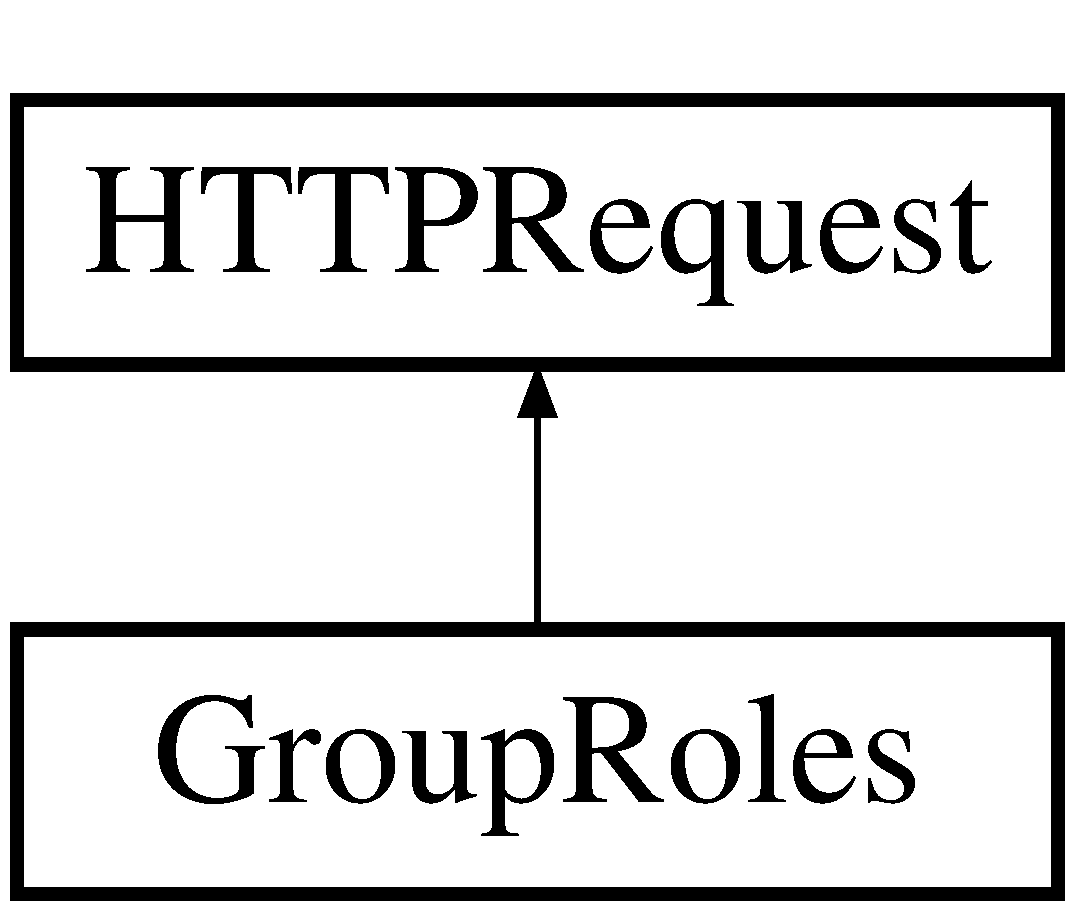
\includegraphics[height=2.000000cm]{classGroupRoles}
\end{center}
\end{figure}
\subsection*{Public Member Functions}
\begin{DoxyCompactItemize}
\item 
\hyperlink{classGroupRoles_a3e20bcdb3805da9903a6a685e540caf6}{\+\_\+\+\_\+construct} (\$galaxy)
\item 
\hyperlink{classGroupRoles_a5105c5645a9de2c49d6c8a4b72687a70}{index} (\$group\+\_\+id)
\item 
\hyperlink{classGroupRoles_a16f189b3452bd6ac8749a937234d0b35}{show} (\$group\+\_\+id, \$role\+\_\+id)
\item 
\hyperlink{classGroupRoles_a1f348f13bc95acfdc2726e70148d8161}{update} (\$group\+\_\+id, \$role\+\_\+id)
\item 
\hyperlink{classGroupRoles_aeaba3d91a004c24198dfd92ab420b231}{delete} (\$group\+\_\+id, \$role\+\_\+id)
\end{DoxyCompactItemize}
\subsection*{Additional Inherited Members}


\subsection{Constructor \& Destructor Documentation}
\index{Group\+Roles@{Group\+Roles}!\+\_\+\+\_\+construct@{\+\_\+\+\_\+construct}}
\index{\+\_\+\+\_\+construct@{\+\_\+\+\_\+construct}!Group\+Roles@{Group\+Roles}}
\subsubsection[{\texorpdfstring{\+\_\+\+\_\+construct(\$galaxy)}{\_\_construct($galaxy)}}]{\setlength{\rightskip}{0pt plus 5cm}Group\+Roles\+::\+\_\+\+\_\+construct (
\begin{DoxyParamCaption}
\item[{}]{\$galaxy}
\end{DoxyParamCaption}
)}\hypertarget{classGroupRoles_a3e20bcdb3805da9903a6a685e540caf6}{}\label{classGroupRoles_a3e20bcdb3805da9903a6a685e540caf6}
The Group \hyperlink{classRoles}{Roles} constructor.


\begin{DoxyParams}[1]{Parameters}
\hyperlink{classGalaxyInstance}{Galaxy\+Instance} & {\em \$galaxy} & A \hyperlink{classGalaxyInstance}{Galaxy\+Instance} object.\\
\hline
\end{DoxyParams}
\begin{DoxyReturn}{Returns}
An instance of a Group \hyperlink{classRoles}{Roles} object. 
\end{DoxyReturn}


\subsection{Member Function Documentation}
\index{Group\+Roles@{Group\+Roles}!delete@{delete}}
\index{delete@{delete}!Group\+Roles@{Group\+Roles}}
\subsubsection[{\texorpdfstring{delete(\$group\+\_\+id, \$role\+\_\+id)}{delete($group\_id, $role\_id)}}]{\setlength{\rightskip}{0pt plus 5cm}Group\+Roles\+::delete (
\begin{DoxyParamCaption}
\item[{}]{\$group\+\_\+id, }
\item[{}]{\$role\+\_\+id}
\end{DoxyParamCaption}
)}\hypertarget{classGroupRoles_aeaba3d91a004c24198dfd92ab420b231}{}\label{classGroupRoles_aeaba3d91a004c24198dfd92ab420b231}
Supports deleting a role from a given group.

Corresponds to the Galaxy A\+PI method and path\+: D\+E\+L\+E\+TE /api/groups/\{encoded\+\_\+group\+\_\+id\}/roles/\{encoded\+\_\+role\+\_\+id\}.


\begin{DoxyParams}{Parameters}
{\em \$group\+\_\+id,The} & id of the group to modify. Group I\+Ds can be found using the \hyperlink{classGroupRoles_a5105c5645a9de2c49d6c8a4b72687a70}{index()} function of this class. \\
\hline
{\em \$role\+\_\+id} & A role id to deassociate any roles from the group. Use the \hyperlink{classRoles}{Roles} class to retreive a list of role I\+Ds. \\
\hline
\end{DoxyParams}
\begin{DoxyReturn}{Returns}
An array of the role that was removed from the group. 
\end{DoxyReturn}
\index{Group\+Roles@{Group\+Roles}!index@{index}}
\index{index@{index}!Group\+Roles@{Group\+Roles}}
\subsubsection[{\texorpdfstring{index(\$group\+\_\+id)}{index($group\_id)}}]{\setlength{\rightskip}{0pt plus 5cm}Group\+Roles\+::index (
\begin{DoxyParamCaption}
\item[{}]{\$group\+\_\+id}
\end{DoxyParamCaption}
)}\hypertarget{classGroupRoles_a5105c5645a9de2c49d6c8a4b72687a70}{}\label{classGroupRoles_a5105c5645a9de2c49d6c8a4b72687a70}
Displays a collection (list) of roles corresponding to a group..

Corresponds to the Galaxy A\+PI method and path\+: G\+ET /api/groups/ \{encoded\+\_\+group\+\_\+id\}/roles.


\begin{DoxyParams}{Parameters}
{\em \$group\+\_\+id} & The id of the group whose roles to list. Group I\+Ds can be found using the \hyperlink{classGroupRoles_a5105c5645a9de2c49d6c8a4b72687a70}{index()} function of the \hyperlink{classGroups}{Groups} class. \\
\hline
\end{DoxyParams}
\begin{DoxyReturn}{Returns}
An array of all group roles for a given group. 
\end{DoxyReturn}
\index{Group\+Roles@{Group\+Roles}!show@{show}}
\index{show@{show}!Group\+Roles@{Group\+Roles}}
\subsubsection[{\texorpdfstring{show(\$group\+\_\+id, \$role\+\_\+id)}{show($group\_id, $role\_id)}}]{\setlength{\rightskip}{0pt plus 5cm}Group\+Roles\+::show (
\begin{DoxyParamCaption}
\item[{}]{\$group\+\_\+id, }
\item[{}]{\$role\+\_\+id}
\end{DoxyParamCaption}
)}\hypertarget{classGroupRoles_a16f189b3452bd6ac8749a937234d0b35}{}\label{classGroupRoles_a16f189b3452bd6ac8749a937234d0b35}
Retreive information about a specific group role.

Corresponds to the Galaxy A\+PI method and path\+: G\+ET /api/groups/\{encoded\+\_\+group\+\_\+id\}/roles/\{encoded\+\_\+role\+\_\+id\}


\begin{DoxyParams}{Parameters}
{\em \$group\+\_\+id} & The id of the group whose roles to list. Group I\+Ds can be found using the \hyperlink{classGroupRoles_a5105c5645a9de2c49d6c8a4b72687a70}{index()} function of the \hyperlink{classGroups}{Groups} class. \\
\hline
{\em \$role\+\_\+id} & The id of the specific role to show. Role I\+DS can be found using the \hyperlink{classGroupRoles_a5105c5645a9de2c49d6c8a4b72687a70}{index()} function of the \hyperlink{classRoles}{Roles} class \\
\hline
\end{DoxyParams}
\begin{DoxyReturn}{Returns}
An array containing details about the role of a given gorup. 
\end{DoxyReturn}
\index{Group\+Roles@{Group\+Roles}!update@{update}}
\index{update@{update}!Group\+Roles@{Group\+Roles}}
\subsubsection[{\texorpdfstring{update(\$group\+\_\+id, \$role\+\_\+id)}{update($group\_id, $role\_id)}}]{\setlength{\rightskip}{0pt plus 5cm}Group\+Roles\+::update (
\begin{DoxyParamCaption}
\item[{}]{\$group\+\_\+id, }
\item[{}]{\$role\+\_\+id}
\end{DoxyParamCaption}
)}\hypertarget{classGroupRoles_a1f348f13bc95acfdc2726e70148d8161}{}\label{classGroupRoles_a1f348f13bc95acfdc2726e70148d8161}
Supports adding a role to a given group.

Corresponds to the Galaxy A\+PI method and path\+: P\+UT /api/groups/\{encoded\+\_\+group\+\_\+id\}/roles/\{encoded\+\_\+role\+\_\+id\}.


\begin{DoxyParams}{Parameters}
{\em \$group\+\_\+id,The} & id of the group to modify. Group I\+Ds can be found using the \hyperlink{classGroupRoles_a5105c5645a9de2c49d6c8a4b72687a70}{index()} function of this class. \\
\hline
{\em \$role\+\_\+id} & A role id to associate any new roles to the group. Use the \hyperlink{classRoles}{Roles} class to retreive a list of existing role I\+Ds. \\
\hline
\end{DoxyParams}
\begin{DoxyReturn}{Returns}
An array of the role that was added to the group 
\end{DoxyReturn}


The documentation for this class was generated from the following file\+:\begin{DoxyCompactItemize}
\item 
\hyperlink{GroupRoles_8inc}{Group\+Roles.\+inc}\end{DoxyCompactItemize}

\hypertarget{classGroups}{}\section{Groups Class Reference}
\label{classGroups}\index{Groups@{Groups}}
Inheritance diagram for Groups\+:\begin{figure}[H]
\begin{center}
\leavevmode
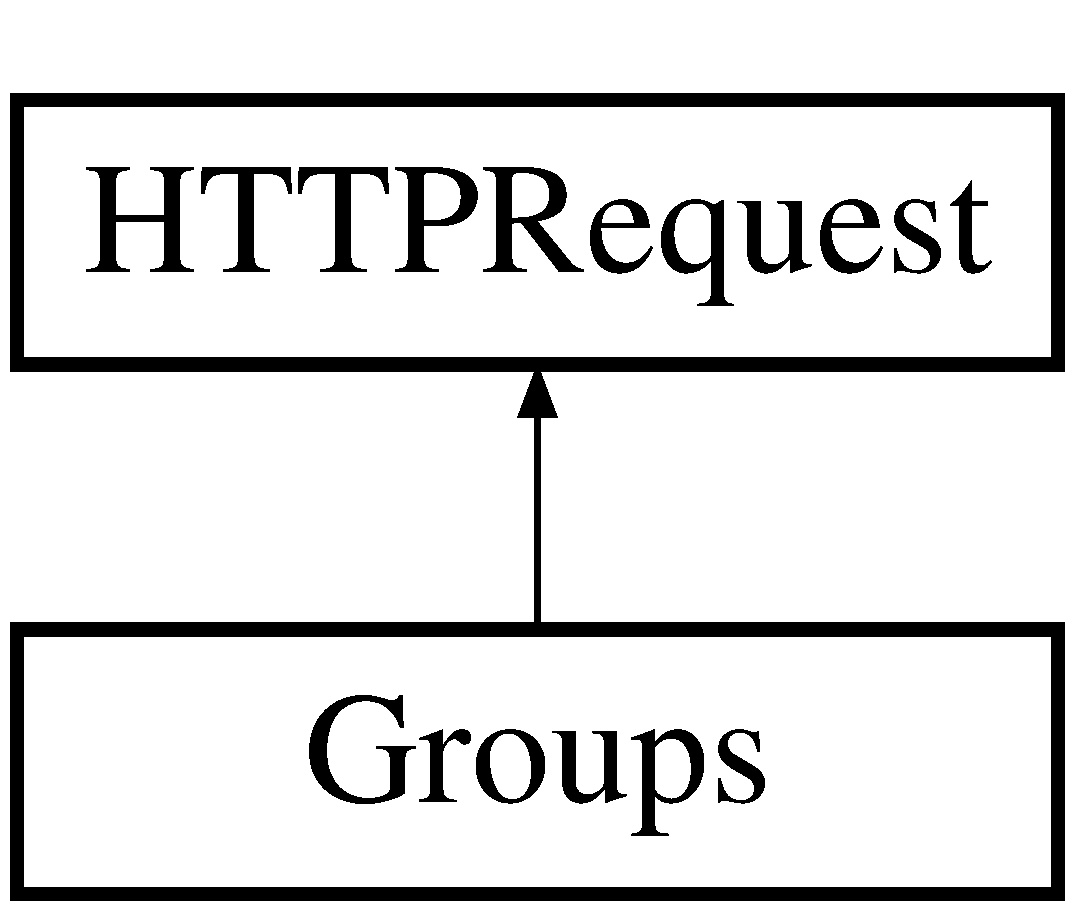
\includegraphics[height=2.000000cm]{classGroups}
\end{center}
\end{figure}
\subsection*{Public Member Functions}
\begin{DoxyCompactItemize}
\item 
\hyperlink{classGroups_a264cd82629a67236a9b575c09baa457c}{\+\_\+\+\_\+construct} (\$galaxy)
\item 
\hyperlink{classGroups_aa86a48d91213d4ef07f3324acb76f088}{index} ()
\item 
\hyperlink{classGroups_a78573fc592f294df38e1754c642bf708}{create} (\$name, \$user\+\_\+ids=array(), \$role\+\_\+ids=array())
\item 
\hyperlink{classGroups_a7000d16e81f12235fe14cf5c1dbea50a}{show} (\$group\+\_\+id)
\item 
\hyperlink{classGroups_ac8a367f511e6bea80962742e9e3e6834}{update} (\$group\+\_\+id, \$name=N\+U\+LL, \$user\+\_\+ids=array(), \$role\+\_\+ids=array())
\end{DoxyCompactItemize}
\subsection*{Additional Inherited Members}


\subsection{Constructor \& Destructor Documentation}
\index{Groups@{Groups}!\+\_\+\+\_\+construct@{\+\_\+\+\_\+construct}}
\index{\+\_\+\+\_\+construct@{\+\_\+\+\_\+construct}!Groups@{Groups}}
\subsubsection[{\texorpdfstring{\+\_\+\+\_\+construct(\$galaxy)}{\_\_construct($galaxy)}}]{\setlength{\rightskip}{0pt plus 5cm}Groups\+::\+\_\+\+\_\+construct (
\begin{DoxyParamCaption}
\item[{}]{\$galaxy}
\end{DoxyParamCaption}
)}\hypertarget{classGroups_a264cd82629a67236a9b575c09baa457c}{}\label{classGroups_a264cd82629a67236a9b575c09baa457c}
The \hyperlink{classGroups}{Groups} constructor.


\begin{DoxyParams}[1]{Parameters}
\hyperlink{classGalaxyInstance}{Galaxy\+Instance} & {\em \$galaxy} & A \hyperlink{classGalaxyInstance}{Galaxy\+Instance} object.\\
\hline
\end{DoxyParams}
\begin{DoxyReturn}{Returns}
An instance of a \hyperlink{classGroups}{Groups} object. 
\end{DoxyReturn}


\subsection{Member Function Documentation}
\index{Groups@{Groups}!create@{create}}
\index{create@{create}!Groups@{Groups}}
\subsubsection[{\texorpdfstring{create(\$name, \$user\+\_\+ids=array(), \$role\+\_\+ids=array())}{create($name, $user\_ids=array(), $role\_ids=array())}}]{\setlength{\rightskip}{0pt plus 5cm}Groups\+::create (
\begin{DoxyParamCaption}
\item[{}]{\$name, }
\item[{}]{\$user\+\_\+ids = {\ttfamily array()}, }
\item[{}]{\$role\+\_\+ids = {\ttfamily array()}}
\end{DoxyParamCaption}
)}\hypertarget{classGroups_a78573fc592f294df38e1754c642bf708}{}\label{classGroups_a78573fc592f294df38e1754c642bf708}
Create a new group.

Corresponds to the Galaxy A\+PI method and path\+: P\+O\+ST /api/groups.


\begin{DoxyParams}{Parameters}
{\em \$name} & Name of the group. \\
\hline
{\em \$user\+\_\+ids} & An array of user\+\_\+ids, if any, to associate user id\textquotesingle{}s to the group. Use the \hyperlink{classUsers}{Users} class to retrieve a list of users. \\
\hline
{\em \$role\+\_\+ids} & An array of role\+\_\+ids to associate any new roles to the group. Use the \hyperlink{classRoles}{Roles} class to retreive a list of existing role I\+Ds.\\
\hline
\end{DoxyParams}
\begin{DoxyReturn}{Returns}
An array of the group that contains the users and roles. 
\end{DoxyReturn}
\index{Groups@{Groups}!index@{index}}
\index{index@{index}!Groups@{Groups}}
\subsubsection[{\texorpdfstring{index()}{index()}}]{\setlength{\rightskip}{0pt plus 5cm}Groups\+::index (
\begin{DoxyParamCaption}
{}
\end{DoxyParamCaption}
)}\hypertarget{classGroups_aa86a48d91213d4ef07f3324acb76f088}{}\label{classGroups_aa86a48d91213d4ef07f3324acb76f088}
Displays a collection (list) of groups.

Corresponds to the Galaxy A\+PI method and path\+: G\+ET /api/groups.

\begin{DoxyReturn}{Returns}
An array of all groups. 
\end{DoxyReturn}
\index{Groups@{Groups}!show@{show}}
\index{show@{show}!Groups@{Groups}}
\subsubsection[{\texorpdfstring{show(\$group\+\_\+id)}{show($group\_id)}}]{\setlength{\rightskip}{0pt plus 5cm}Groups\+::show (
\begin{DoxyParamCaption}
\item[{}]{\$group\+\_\+id}
\end{DoxyParamCaption}
)}\hypertarget{classGroups_a7000d16e81f12235fe14cf5c1dbea50a}{}\label{classGroups_a7000d16e81f12235fe14cf5c1dbea50a}
Retreive information about a group.

Corresponds to the Galaxy A\+PI method and path\+: G\+ET /api/groups/\{encoded\+\_\+group\+\_\+id\}


\begin{DoxyParams}{Parameters}
{\em \$group\+\_\+id} & The id of the specific group to show. Group I\+Ds can be found using the \hyperlink{classGroups_aa86a48d91213d4ef07f3324acb76f088}{index()} function of this class. \\
\hline
\end{DoxyParams}
\begin{DoxyReturn}{Returns}
An array containing details about the group. 
\end{DoxyReturn}
\index{Groups@{Groups}!update@{update}}
\index{update@{update}!Groups@{Groups}}
\subsubsection[{\texorpdfstring{update(\$group\+\_\+id, \$name=\+N\+U\+L\+L, \$user\+\_\+ids=array(), \$role\+\_\+ids=array())}{update($group\_id, $name=NULL, $user\_ids=array(), $role\_ids=array())}}]{\setlength{\rightskip}{0pt plus 5cm}Groups\+::update (
\begin{DoxyParamCaption}
\item[{}]{\$group\+\_\+id, }
\item[{}]{\$name = {\ttfamily NULL}, }
\item[{}]{\$user\+\_\+ids = {\ttfamily array()}, }
\item[{}]{\$role\+\_\+ids = {\ttfamily array()}}
\end{DoxyParamCaption}
)}\hypertarget{classGroups_ac8a367f511e6bea80962742e9e3e6834}{}\label{classGroups_ac8a367f511e6bea80962742e9e3e6834}
Supports changes to a group including the name, users and roles.

Corresponds to the Galaxy A\+PI method and path\+: P\+O\+ST /api/groups/\{encoded\+\_\+group\+\_\+id\}.


\begin{DoxyParams}{Parameters}
{\em \$group\+\_\+id,The} & id of the group to modify. Group I\+Ds can be found using the \hyperlink{classGroups_aa86a48d91213d4ef07f3324acb76f088}{index()} function of this class. \\
\hline
{\em \$name,A} & new name, if any, to call the group. \\
\hline
{\em \$user\+\_\+ids} & An array of user\+\_\+ids, if any, to associate user id\textquotesingle{}s to the group. Use the \hyperlink{classUsers}{Users} class to retrieve a list of users. \\
\hline
{\em \$role\+\_\+ids} & An array of role\+\_\+ids to associate any new roles to the group. Use the \hyperlink{classRoles}{Roles} class to retreive a list of existing role I\+Ds.\\
\hline
\end{DoxyParams}
\begin{DoxyReturn}{Returns}
An array of the group that contains the users and roles. 
\end{DoxyReturn}


The documentation for this class was generated from the following file\+:\begin{DoxyCompactItemize}
\item 
\hyperlink{Groups_8inc}{Groups.\+inc}\end{DoxyCompactItemize}

\hypertarget{classGroupUsers}{}\section{Group\+Users Class Reference}
\label{classGroupUsers}\index{Group\+Users@{Group\+Users}}
Inheritance diagram for Group\+Users\+:\begin{figure}[H]
\begin{center}
\leavevmode
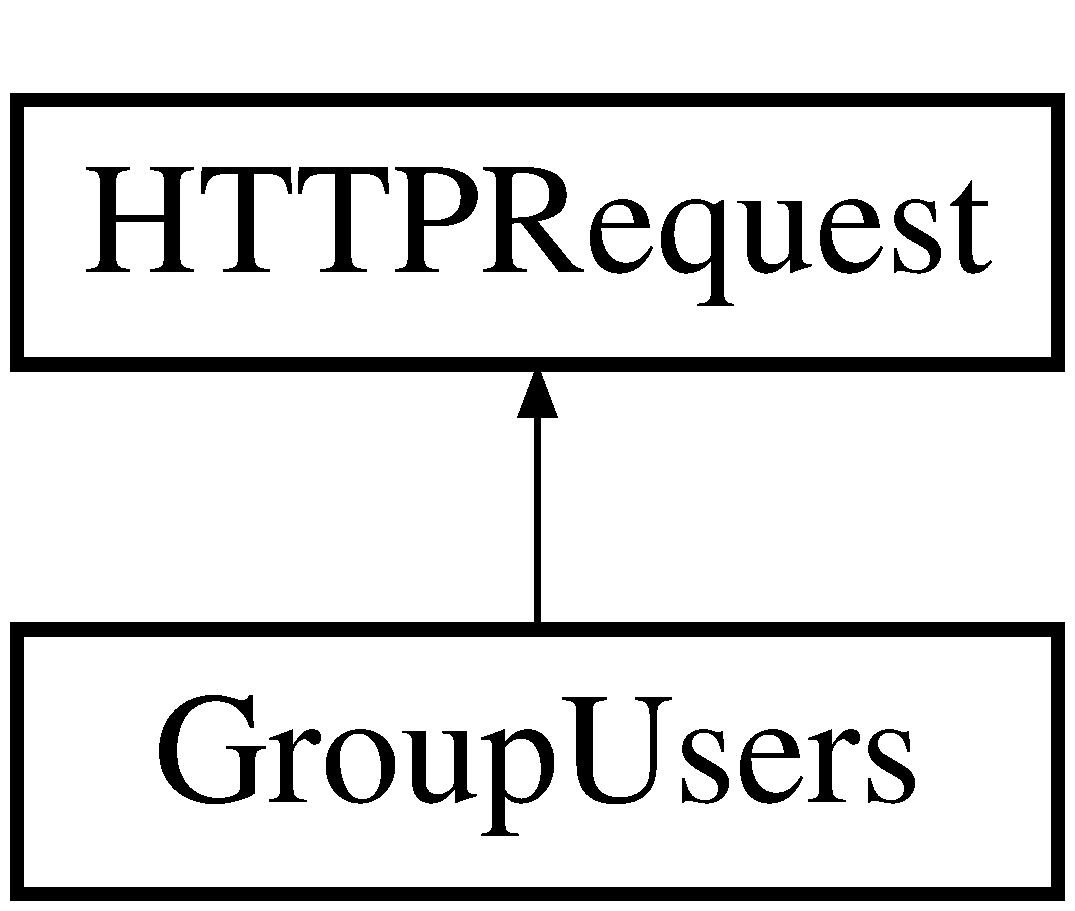
\includegraphics[height=2.000000cm]{classGroupUsers}
\end{center}
\end{figure}
\subsection*{Public Member Functions}
\begin{DoxyCompactItemize}
\item 
\hyperlink{classGroupUsers_a125d93cc05e8407a2a583af2610e0698}{\+\_\+\+\_\+construct} (\$galaxy)
\item 
\hyperlink{classGroupUsers_a8369879632f0a6a70ca0cc1c10b212c0}{index} (\$group\+\_\+id)
\item 
\hyperlink{classGroupUsers_a49efdc7af6b1674c2c801189bde705c9}{show} (\$group\+\_\+id, \$user\+\_\+id)
\item 
\hyperlink{classGroupUsers_a2071b9abb888043c786a9a703aace443}{update} (\$group\+\_\+id, \$user\+\_\+id)
\item 
\hyperlink{classGroupUsers_a2b6abd239c7f8819ba0dfa9a5d904bb6}{delete} (\$group\+\_\+id, \$user\+\_\+id)
\end{DoxyCompactItemize}
\subsection*{Additional Inherited Members}


\subsection{Constructor \& Destructor Documentation}
\index{Group\+Users@{Group\+Users}!\+\_\+\+\_\+construct@{\+\_\+\+\_\+construct}}
\index{\+\_\+\+\_\+construct@{\+\_\+\+\_\+construct}!Group\+Users@{Group\+Users}}
\subsubsection[{\texorpdfstring{\+\_\+\+\_\+construct(\$galaxy)}{\_\_construct($galaxy)}}]{\setlength{\rightskip}{0pt plus 5cm}Group\+Users\+::\+\_\+\+\_\+construct (
\begin{DoxyParamCaption}
\item[{}]{\$galaxy}
\end{DoxyParamCaption}
)}\hypertarget{classGroupUsers_a125d93cc05e8407a2a583af2610e0698}{}\label{classGroupUsers_a125d93cc05e8407a2a583af2610e0698}
The \hyperlink{classGroupUsers}{Group\+Users} constructor.


\begin{DoxyParams}[1]{Parameters}
\hyperlink{classGalaxyInstance}{Galaxy\+Instance} & {\em \$galaxy} & A \hyperlink{classGalaxyInstance}{Galaxy\+Instance} object.\\
\hline
\end{DoxyParams}
\begin{DoxyReturn}{Returns}
An instance of a \hyperlink{classGroups}{Groups} \hyperlink{classUsers}{Users} object. 
\end{DoxyReturn}


\subsection{Member Function Documentation}
\index{Group\+Users@{Group\+Users}!delete@{delete}}
\index{delete@{delete}!Group\+Users@{Group\+Users}}
\subsubsection[{\texorpdfstring{delete(\$group\+\_\+id, \$user\+\_\+id)}{delete($group\_id, $user\_id)}}]{\setlength{\rightskip}{0pt plus 5cm}Group\+Users\+::delete (
\begin{DoxyParamCaption}
\item[{}]{\$group\+\_\+id, }
\item[{}]{\$user\+\_\+id}
\end{DoxyParamCaption}
)}\hypertarget{classGroupUsers_a2b6abd239c7f8819ba0dfa9a5d904bb6}{}\label{classGroupUsers_a2b6abd239c7f8819ba0dfa9a5d904bb6}
Deletes a user from a given group.

Corresponds to the Galaxy A\+PI method and path\+: D\+E\+L\+E\+TE /api/groups/\{encoded\+\_\+group\+\_\+id\}/users/\{encoded\+\_\+user\+\_\+id\}.


\begin{DoxyParams}{Parameters}
{\em \$group\+\_\+id,The} & id of the group to modify. Group I\+Ds can be found using the \hyperlink{classGroupUsers_a8369879632f0a6a70ca0cc1c10b212c0}{index()} function of this class. \\
\hline
{\em \$user\+\_\+id} & A user id to deassociate any users from the group. Use the \hyperlink{classUsers}{Users} class to retreive a list of user I\+Ds. \\
\hline
\end{DoxyParams}
\begin{DoxyReturn}{Returns}
An array of the user that has been removed from the group. 
\end{DoxyReturn}
\index{Group\+Users@{Group\+Users}!index@{index}}
\index{index@{index}!Group\+Users@{Group\+Users}}
\subsubsection[{\texorpdfstring{index(\$group\+\_\+id)}{index($group\_id)}}]{\setlength{\rightskip}{0pt plus 5cm}Group\+Users\+::index (
\begin{DoxyParamCaption}
\item[{}]{\$group\+\_\+id}
\end{DoxyParamCaption}
)}\hypertarget{classGroupUsers_a8369879632f0a6a70ca0cc1c10b212c0}{}\label{classGroupUsers_a8369879632f0a6a70ca0cc1c10b212c0}
Displays a collection (list) of users corresponding to a group..

Corresponds to the Galaxy A\+PI method and path\+: G\+ET /api/groups/ \{encoded\+\_\+group\+\_\+id\}/users.


\begin{DoxyParams}{Parameters}
{\em \$group\+\_\+id} & The id of the group whose users to list. Group I\+Ds can be found using the \hyperlink{classGroupUsers_a8369879632f0a6a70ca0cc1c10b212c0}{index()} function of the \hyperlink{classGroups}{Groups} class. \\
\hline
\end{DoxyParams}
\begin{DoxyReturn}{Returns}
An array of all users of a given group. 
\end{DoxyReturn}
\index{Group\+Users@{Group\+Users}!show@{show}}
\index{show@{show}!Group\+Users@{Group\+Users}}
\subsubsection[{\texorpdfstring{show(\$group\+\_\+id, \$user\+\_\+id)}{show($group\_id, $user\_id)}}]{\setlength{\rightskip}{0pt plus 5cm}Group\+Users\+::show (
\begin{DoxyParamCaption}
\item[{}]{\$group\+\_\+id, }
\item[{}]{\$user\+\_\+id}
\end{DoxyParamCaption}
)}\hypertarget{classGroupUsers_a49efdc7af6b1674c2c801189bde705c9}{}\label{classGroupUsers_a49efdc7af6b1674c2c801189bde705c9}
Retreive information about a specific group user.

Corresponds to the Galaxy A\+PI method and path\+: G\+ET /api/groups/\{encoded\+\_\+group\+\_\+id\}/users/\{encoded\+\_\+user\+\_\+id\}


\begin{DoxyParams}{Parameters}
{\em \$group\+\_\+id} & The id of the group whose users to list. Group I\+Ds can be found using the \hyperlink{classGroupUsers_a8369879632f0a6a70ca0cc1c10b212c0}{index()} function of the \hyperlink{classGroups}{Groups} class. \\
\hline
{\em \$user\+\_\+id} & The id of the specific user to show. User I\+DS can be found using the \hyperlink{classGroupUsers_a8369879632f0a6a70ca0cc1c10b212c0}{index()} function of the \hyperlink{classUsers}{Users} class \\
\hline
\end{DoxyParams}
\begin{DoxyReturn}{Returns}
An array containing details about the user of a given group. 
\end{DoxyReturn}
\index{Group\+Users@{Group\+Users}!update@{update}}
\index{update@{update}!Group\+Users@{Group\+Users}}
\subsubsection[{\texorpdfstring{update(\$group\+\_\+id, \$user\+\_\+id)}{update($group\_id, $user\_id)}}]{\setlength{\rightskip}{0pt plus 5cm}Group\+Users\+::update (
\begin{DoxyParamCaption}
\item[{}]{\$group\+\_\+id, }
\item[{}]{\$user\+\_\+id}
\end{DoxyParamCaption}
)}\hypertarget{classGroupUsers_a2071b9abb888043c786a9a703aace443}{}\label{classGroupUsers_a2071b9abb888043c786a9a703aace443}
Adds a user to a given group.

Corresponds to the Galaxy A\+PI method and path\+: P\+UT /api/groups/\{encoded\+\_\+group\+\_\+id\}/users/\{encoded\+\_\+user\+\_\+id\}.


\begin{DoxyParams}{Parameters}
{\em \$group\+\_\+id,The} & id of the group to modify. Group I\+Ds can be found using the \hyperlink{classGroupUsers_a8369879632f0a6a70ca0cc1c10b212c0}{index()} function of this class. \\
\hline
{\em \$user\+\_\+id} & A user id to associate any new users to the group. Use the \hyperlink{classUsers}{Users} class to retreive a list of existing user I\+Ds. \\
\hline
\end{DoxyParams}
\begin{DoxyReturn}{Returns}
An array of the user that has added to the group 
\end{DoxyReturn}


The documentation for this class was generated from the following file\+:\begin{DoxyCompactItemize}
\item 
\hyperlink{GroupUsers_8inc}{Group\+Users.\+inc}\end{DoxyCompactItemize}

\hypertarget{classHistories}{}\section{Histories Class Reference}
\label{classHistories}\index{Histories@{Histories}}
Inheritance diagram for Histories\+:\begin{figure}[H]
\begin{center}
\leavevmode
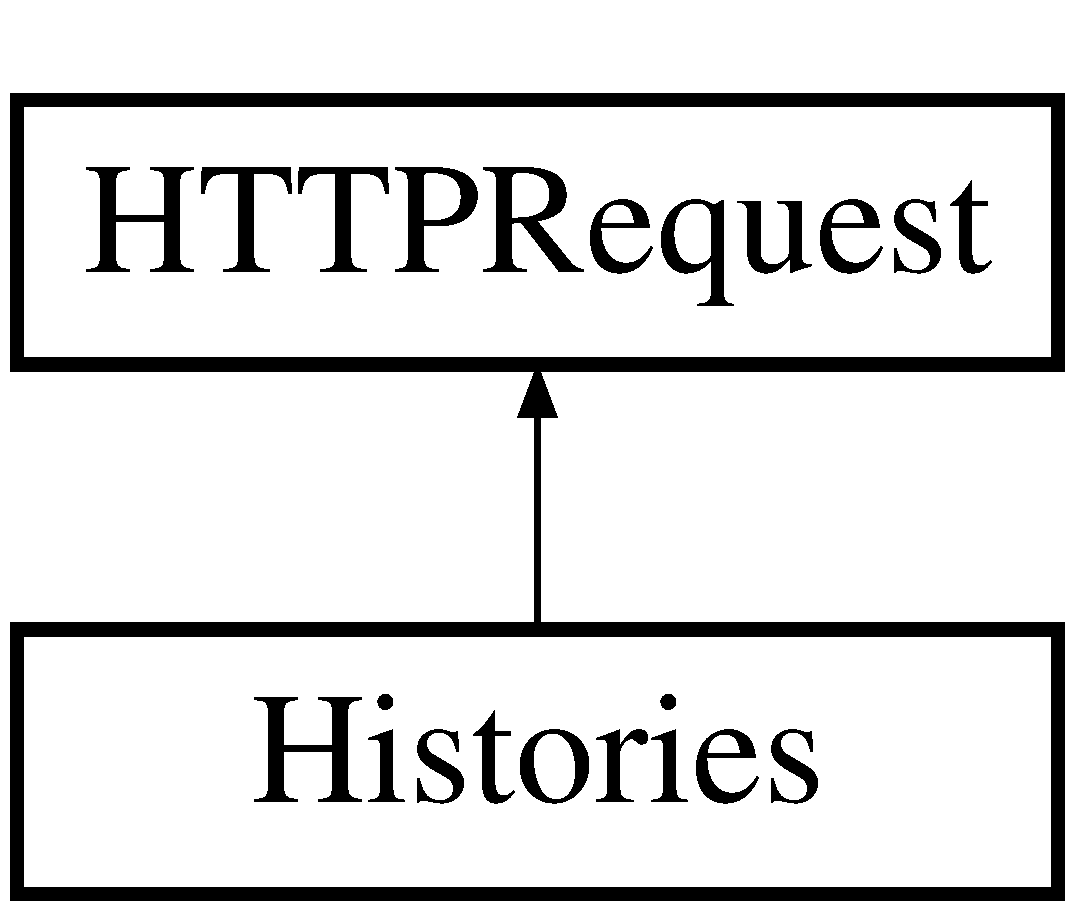
\includegraphics[height=2.000000cm]{classHistories}
\end{center}
\end{figure}
\subsection*{Public Member Functions}
\begin{DoxyCompactItemize}
\item 
\hyperlink{classHistories_a27eb8affae85703d91bcb7d617209e66}{\+\_\+\+\_\+construct} (\$galaxy)
\item 
\hyperlink{classHistories_a69e4b7e9bde24290c1d40c29cd69a358}{create} (\$name, \$history\+\_\+id=N\+U\+LL, \$archive\+\_\+source=N\+U\+LL, \$archive\+\_\+type=N\+U\+LL, \$all\+\_\+datasets=T\+R\+UE)
\item 
\hyperlink{classHistories_a43a92a2839e481a5f39b6444971e616f}{index} ()
\item 
\hyperlink{classHistories_a5f32d9aa6597f3876fc9291614dae85a}{show} (\$history\+\_\+id)
\item 
\hyperlink{classHistories_acbd17070f53a4326029374878760846d}{archive\+Download} (\$history\+\_\+id, \$file\+\_\+path)
\item 
\hyperlink{classHistories_addacbe6d8744835911f6547d4b935b41}{archive\+Export} (\$history\+\_\+id)
\item 
\hyperlink{classHistories_a97773d15901aea83dc44ea8d15e98e8b}{delete\+History} (\$history\+\_\+id)
\item 
\hyperlink{classHistories_aa0317b96601a7a6b4ca607770714c821}{undelete} (\$history\+\_\+id)
\item 
\hyperlink{classHistories_aa613fec2475a87da10e7cabc7cf3b4c0}{citations} (\$history\+\_\+id)
\item 
\hyperlink{classHistories_a6fbbf74042939c393cf7163b481cd0b1}{published} ()
\item 
\hyperlink{classHistories_af5cc87c475e5b864af68772dd3329a82}{shared\+With\+Me} ()
\end{DoxyCompactItemize}
\subsection*{Additional Inherited Members}


\subsection{Constructor \& Destructor Documentation}
\index{Histories@{Histories}!\+\_\+\+\_\+construct@{\+\_\+\+\_\+construct}}
\index{\+\_\+\+\_\+construct@{\+\_\+\+\_\+construct}!Histories@{Histories}}
\subsubsection[{\texorpdfstring{\+\_\+\+\_\+construct(\$galaxy)}{\_\_construct($galaxy)}}]{\setlength{\rightskip}{0pt plus 5cm}Histories\+::\+\_\+\+\_\+construct (
\begin{DoxyParamCaption}
\item[{}]{\$galaxy}
\end{DoxyParamCaption}
)}\hypertarget{classHistories_a27eb8affae85703d91bcb7d617209e66}{}\label{classHistories_a27eb8affae85703d91bcb7d617209e66}
The \hyperlink{classHistories}{Histories} constructor.


\begin{DoxyParams}[1]{Parameters}
\hyperlink{classGalaxyInstance}{Galaxy\+Instance} & {\em \$galaxy} & A \hyperlink{classGalaxyInstance}{Galaxy\+Instance} object.\\
\hline
\end{DoxyParams}
\begin{DoxyReturn}{Returns}
An instance of a \hyperlink{classHistories}{Histories} object. 
\end{DoxyReturn}


\subsection{Member Function Documentation}
\index{Histories@{Histories}!archive\+Download@{archive\+Download}}
\index{archive\+Download@{archive\+Download}!Histories@{Histories}}
\subsubsection[{\texorpdfstring{archive\+Download(\$history\+\_\+id, \$file\+\_\+path)}{archiveDownload($history\_id, $file\_path)}}]{\setlength{\rightskip}{0pt plus 5cm}Histories\+::archive\+Download (
\begin{DoxyParamCaption}
\item[{}]{\$history\+\_\+id, }
\item[{}]{\$file\+\_\+path}
\end{DoxyParamCaption}
)}\hypertarget{classHistories_acbd17070f53a4326029374878760846d}{}\label{classHistories_acbd17070f53a4326029374878760846d}
Download a given history with indicated history id.

Corresponds to the Galaxy A\+PI method and path\+:

P\+UT /api/histories/\{id\}/exports\textquotesingle{} and\+: G\+ET /api/histories/\{id\}/exports/\{jeha\+\_\+id\}


\begin{DoxyParams}{Parameters}
{\em \$history\+\_\+id} & The id of the history to download To obtain history\+\_\+id\textquotesingle{}s, please use this classes\textquotesingle{} \hyperlink{classHistories_a43a92a2839e481a5f39b6444971e616f}{index()} function. \\
\hline
{\em \$file\+\_\+path} & The full path (including the file name) on the file systems where this file should be written. Ideally, the file name should have a .tar.\+gz extension as the downloaded file is tar\textquotesingle{}ed and gzip compressed.\\
\hline
\end{DoxyParams}
\begin{DoxyReturn}{Returns}
T\+R\+UE if the download was successful and F\+A\+L\+SE otherwise. 
\end{DoxyReturn}
\index{Histories@{Histories}!archive\+Export@{archive\+Export}}
\index{archive\+Export@{archive\+Export}!Histories@{Histories}}
\subsubsection[{\texorpdfstring{archive\+Export(\$history\+\_\+id)}{archiveExport($history\_id)}}]{\setlength{\rightskip}{0pt plus 5cm}Histories\+::archive\+Export (
\begin{DoxyParamCaption}
\item[{}]{\$history\+\_\+id}
\end{DoxyParamCaption}
)}\hypertarget{classHistories_addacbe6d8744835911f6547d4b935b41}{}\label{classHistories_addacbe6d8744835911f6547d4b935b41}
Start Job to create history export for corresponding history.

Corresponds to the Galaxy A\+PI method and path\+: P\+UT /api/histories/\{id\}/exports\+:


\begin{DoxyParams}{Parameters}
{\em \$history\+\_\+id} & the encoded id of the history to export.\\
\hline
\end{DoxyParams}
\begin{DoxyReturn}{Returns}
A U\+RL of where to download the export. 
\end{DoxyReturn}
\index{Histories@{Histories}!citations@{citations}}
\index{citations@{citations}!Histories@{Histories}}
\subsubsection[{\texorpdfstring{citations(\$history\+\_\+id)}{citations($history\_id)}}]{\setlength{\rightskip}{0pt plus 5cm}Histories\+::citations (
\begin{DoxyParamCaption}
\item[{}]{\$history\+\_\+id}
\end{DoxyParamCaption}
)}\hypertarget{classHistories_aa613fec2475a87da10e7cabc7cf3b4c0}{}\label{classHistories_aa613fec2475a87da10e7cabc7cf3b4c0}
Retreive information of the citations of a specified history.

Corresponds to the Galaxy A\+PI method and path\+: G\+ET /api/histories/\{encoded\+\_\+history\+\_\+id\}/citations


\begin{DoxyParams}{Parameters}
{\em history\+\_\+id} & The encoded id of the history to undelete. To obtain history\+\_\+id\textquotesingle{}s, please use this classes\textquotesingle{} \hyperlink{classHistories_a43a92a2839e481a5f39b6444971e616f}{index()} function.\\
\hline
\end{DoxyParams}
\begin{DoxyReturn}{Returns}
An array of citations. 
\end{DoxyReturn}
\index{Histories@{Histories}!create@{create}}
\index{create@{create}!Histories@{Histories}}
\subsubsection[{\texorpdfstring{create(\$name, \$history\+\_\+id=\+N\+U\+L\+L, \$archive\+\_\+source=\+N\+U\+L\+L, \$archive\+\_\+type=\+N\+U\+L\+L, \$all\+\_\+datasets=\+T\+R\+U\+E)}{create($name, $history\_id=NULL, $archive\_source=NULL, $archive\_type=NULL, $all\_datasets=TRUE)}}]{\setlength{\rightskip}{0pt plus 5cm}Histories\+::create (
\begin{DoxyParamCaption}
\item[{}]{\$name, }
\item[{}]{\$history\+\_\+id = {\ttfamily NULL}, }
\item[{}]{\$archive\+\_\+source = {\ttfamily NULL}, }
\item[{}]{\$archive\+\_\+type = {\ttfamily NULL}, }
\item[{}]{\$all\+\_\+datasets = {\ttfamily TRUE}}
\end{DoxyParamCaption}
)}\hypertarget{classHistories_a69e4b7e9bde24290c1d40c29cd69a358}{}\label{classHistories_a69e4b7e9bde24290c1d40c29cd69a358}
Create a new History component in Galaxy.

Corresponds to the Galaxy A\+PI method and path\+: P\+O\+ST /api/histories\+:

Creates a new history in a galaxy instance Note the option to pass \textquotesingle{}keys\textquotesingle{} and \textquotesingle{}views\textquotesingle{} is currently not supported


\begin{DoxyParams}{Parameters}
{\em name} & The new history\textquotesingle{}s name \\
\hline
{\em history\+\_\+id} & The id of the history to copy (will copy contents to new history) To obtain history\+\_\+id\textquotesingle{}s, please use this classes\textquotesingle{} \hyperlink{classHistories_a43a92a2839e481a5f39b6444971e616f}{index()} function. \\
\hline
{\em archive\+\_\+source} & The url that will generate the archive to import. \\
\hline
{\em archive\+\_\+type} & \textquotesingle{}url\textquotesingle{} (default) \\
\hline
{\em bool} & all\+\_\+datasets Copy deleted hdas/hdcas \textquotesingle{}True\textquotesingle{} or \textquotesingle{}False\textquotesingle{}, defaults to True.\\
\hline
\end{DoxyParams}
\begin{DoxyReturn}{Returns}
An array containing information about the new History component. 
\end{DoxyReturn}
\index{Histories@{Histories}!delete\+History@{delete\+History}}
\index{delete\+History@{delete\+History}!Histories@{Histories}}
\subsubsection[{\texorpdfstring{delete\+History(\$history\+\_\+id)}{deleteHistory($history\_id)}}]{\setlength{\rightskip}{0pt plus 5cm}Histories\+::delete\+History (
\begin{DoxyParamCaption}
\item[{}]{\$history\+\_\+id}
\end{DoxyParamCaption}
)}\hypertarget{classHistories_a97773d15901aea83dc44ea8d15e98e8b}{}\label{classHistories_a97773d15901aea83dc44ea8d15e98e8b}
Delete a specified history.

Corresponds to the Galaxy A\+PI method and path\+: D\+E\+L\+E\+TE /api/histories/\{encoded\+\_\+history\+\_\+id\}


\begin{DoxyParams}{Parameters}
{\em history\+\_\+id} & The encoded id of the history to delete. To obtain history\+\_\+id\textquotesingle{}s, please use this classes\textquotesingle{} \hyperlink{classHistories_a43a92a2839e481a5f39b6444971e616f}{index()} function.\\
\hline
\end{DoxyParams}
\begin{DoxyReturn}{Returns}
An array of deleted histories. 
\end{DoxyReturn}
\index{Histories@{Histories}!index@{index}}
\index{index@{index}!Histories@{Histories}}
\subsubsection[{\texorpdfstring{index()}{index()}}]{\setlength{\rightskip}{0pt plus 5cm}Histories\+::index (
\begin{DoxyParamCaption}
{}
\end{DoxyParamCaption}
)}\hypertarget{classHistories_a43a92a2839e481a5f39b6444971e616f}{}\label{classHistories_a43a92a2839e481a5f39b6444971e616f}
Displays a collection of history components in Galaxy.

This function combines the list of active and deleted histories and therefore, corresponds to both of the Galaxy A\+PI methods and paths\+:

G\+ET /api/histories and G\+ET /api/histories/deleted

\begin{DoxyReturn}{Returns}
An array containing list of histories in galaxy instance. 
\end{DoxyReturn}
\index{Histories@{Histories}!published@{published}}
\index{published@{published}!Histories@{Histories}}
\subsubsection[{\texorpdfstring{published()}{published()}}]{\setlength{\rightskip}{0pt plus 5cm}Histories\+::published (
\begin{DoxyParamCaption}
{}
\end{DoxyParamCaption}
)}\hypertarget{classHistories_a6fbbf74042939c393cf7163b481cd0b1}{}\label{classHistories_a6fbbf74042939c393cf7163b481cd0b1}
Retreive all histories that have been published.

Corresponds to the Galaxy A\+PI method and path\+: G\+ET /api/histories/published\+:

\begin{DoxyReturn}{Returns}
An array of published histories. 
\end{DoxyReturn}
\index{Histories@{Histories}!shared\+With\+Me@{shared\+With\+Me}}
\index{shared\+With\+Me@{shared\+With\+Me}!Histories@{Histories}}
\subsubsection[{\texorpdfstring{shared\+With\+Me()}{sharedWithMe()}}]{\setlength{\rightskip}{0pt plus 5cm}Histories\+::shared\+With\+Me (
\begin{DoxyParamCaption}
{}
\end{DoxyParamCaption}
)}\hypertarget{classHistories_af5cc87c475e5b864af68772dd3329a82}{}\label{classHistories_af5cc87c475e5b864af68772dd3329a82}
Retreive all histories that are shared with the current user.

Corresponds to the Galaxy A\+PI method and path\+: G\+ET /api/histories/shared\+\_\+with\+\_\+me\+:

\begin{DoxyReturn}{Returns}
An array histories shared with the current user. 
\end{DoxyReturn}
\index{Histories@{Histories}!show@{show}}
\index{show@{show}!Histories@{Histories}}
\subsubsection[{\texorpdfstring{show(\$history\+\_\+id)}{show($history\_id)}}]{\setlength{\rightskip}{0pt plus 5cm}Histories\+::show (
\begin{DoxyParamCaption}
\item[{}]{\$history\+\_\+id}
\end{DoxyParamCaption}
)}\hypertarget{classHistories_a5f32d9aa6597f3876fc9291614dae85a}{}\label{classHistories_a5f32d9aa6597f3876fc9291614dae85a}
Retreive detailed information about a particular history component.

Corresponds to the Galaxy A\+PI method and path\+: P\+O\+ST /api/histories/\{encoded\+\_\+history\+\_\+id\}\+:


\begin{DoxyParams}{Parameters}
{\em history\+\_\+id} & The id of the history to retreive. To obtain history\+\_\+id\textquotesingle{}s, please use this classes\textquotesingle{} \hyperlink{classHistories_a43a92a2839e481a5f39b6444971e616f}{index()} function.\\
\hline
\end{DoxyParams}
\begin{DoxyReturn}{Returns}
Json array containing information about the specified history 
\end{DoxyReturn}
\index{Histories@{Histories}!undelete@{undelete}}
\index{undelete@{undelete}!Histories@{Histories}}
\subsubsection[{\texorpdfstring{undelete(\$history\+\_\+id)}{undelete($history\_id)}}]{\setlength{\rightskip}{0pt plus 5cm}Histories\+::undelete (
\begin{DoxyParamCaption}
\item[{}]{\$history\+\_\+id}
\end{DoxyParamCaption}
)}\hypertarget{classHistories_aa0317b96601a7a6b4ca607770714c821}{}\label{classHistories_aa0317b96601a7a6b4ca607770714c821}
Undelete a specified history.

Corresponds to the Galaxy A\+PI method and path\+: D\+E\+L\+E\+TE /api/histories/deleted/\{encoded\+\_\+history\+\_\+id\}


\begin{DoxyParams}{Parameters}
{\em history\+\_\+id} & The encoded id of the history to undelete. To obtain history\+\_\+id\textquotesingle{}s, please use this classes\textquotesingle{} \hyperlink{classHistories_a43a92a2839e481a5f39b6444971e616f}{index()} function.\\
\hline
\end{DoxyParams}
\begin{DoxyReturn}{Returns}
An array of undeleted histories. 
\end{DoxyReturn}


The documentation for this class was generated from the following file\+:\begin{DoxyCompactItemize}
\item 
\hyperlink{Histories_8inc}{Histories.\+inc}\end{DoxyCompactItemize}

\hypertarget{classHistoryContents}{}\section{History\+Contents Class Reference}
\label{classHistoryContents}\index{History\+Contents@{History\+Contents}}
Inheritance diagram for History\+Contents\+:\begin{figure}[H]
\begin{center}
\leavevmode
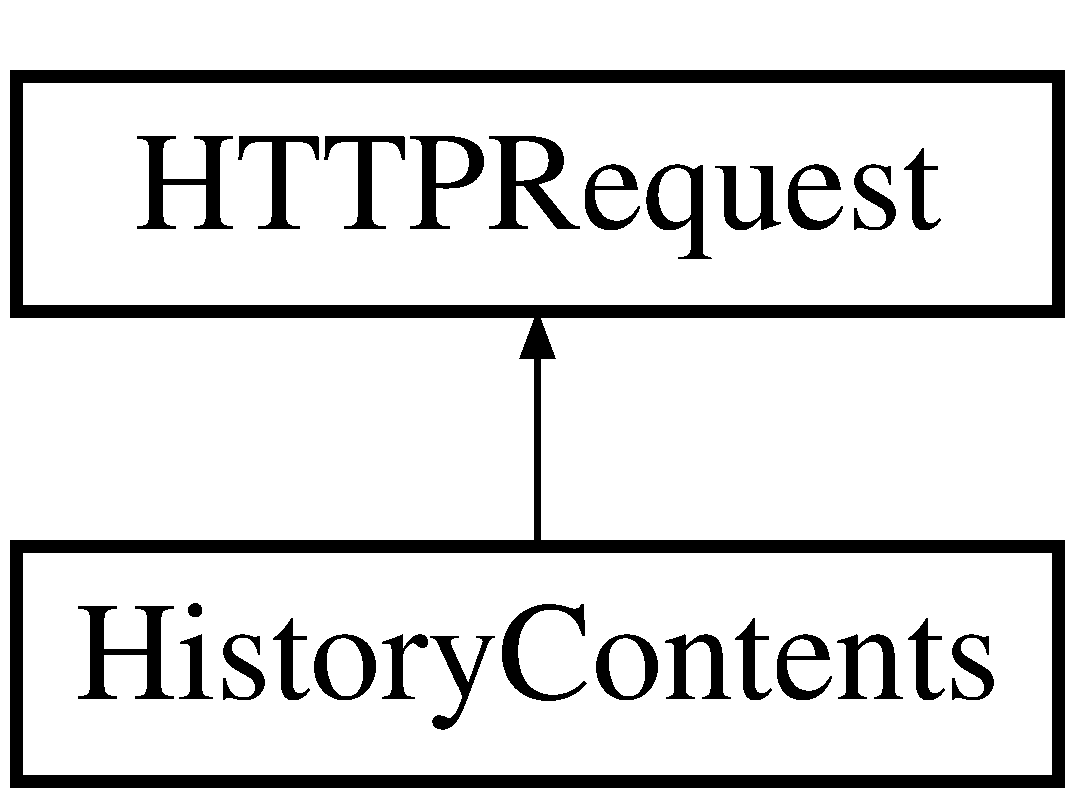
\includegraphics[height=2.000000cm]{classHistoryContents}
\end{center}
\end{figure}
\subsection*{Public Member Functions}
\begin{DoxyCompactItemize}
\item 
\hyperlink{classHistoryContents_a3ea1e946ae6dbcb3d679e29154e69676}{\+\_\+\+\_\+construct} (\$galaxy)
\item 
\hyperlink{classHistoryContents_ac2e074468ce3b73a9463adec372ebe91}{create} (\$history\+\_\+id, \$content\+\_\+id, \$source=\textquotesingle{}hda\textquotesingle{})
\item 
\hyperlink{classHistoryContents_a5729d3c11cf8c8e3d317c802694ff633}{show} (\$history\+\_\+id, \$content\+\_\+id)
\item 
\hyperlink{classHistoryContents_aa38324b7aa0f92ae7ce26083fe8c2972}{update} (\$history\+\_\+id, \$content\+\_\+id, \$annotation=\textquotesingle{}\textquotesingle{})
\item 
\hyperlink{classHistoryContents_a53ffc8a65942b92724e248de38bdfe2b}{delete} (\$history\+\_\+id, \$content\+\_\+id, \$purge=false)
\item 
\hyperlink{classHistoryContents_aa8f0cc4cf1b594d6fc485b2f94a57b89}{index} (\$history\+\_\+id, \$ids=N\+U\+LL)
\end{DoxyCompactItemize}
\subsection*{Additional Inherited Members}


\subsection{Constructor \& Destructor Documentation}
\index{History\+Contents@{History\+Contents}!\+\_\+\+\_\+construct@{\+\_\+\+\_\+construct}}
\index{\+\_\+\+\_\+construct@{\+\_\+\+\_\+construct}!History\+Contents@{History\+Contents}}
\subsubsection[{\texorpdfstring{\+\_\+\+\_\+construct(\$galaxy)}{\_\_construct($galaxy)}}]{\setlength{\rightskip}{0pt plus 5cm}History\+Contents\+::\+\_\+\+\_\+construct (
\begin{DoxyParamCaption}
\item[{}]{\$galaxy}
\end{DoxyParamCaption}
)}\hypertarget{classHistoryContents_a3ea1e946ae6dbcb3d679e29154e69676}{}\label{classHistoryContents_a3ea1e946ae6dbcb3d679e29154e69676}
The \hyperlink{classHistoryContents}{History\+Contents} constructor.


\begin{DoxyParams}[1]{Parameters}
\hyperlink{classGalaxyInstance}{Galaxy\+Instance} & {\em \$galaxy} & A \hyperlink{classGalaxyInstance}{Galaxy\+Instance} object.\\
\hline
\end{DoxyParams}
\begin{DoxyReturn}{Returns}
An instance of a \hyperlink{classHistoryContents}{History\+Contents} object. 
\end{DoxyReturn}


\subsection{Member Function Documentation}
\index{History\+Contents@{History\+Contents}!create@{create}}
\index{create@{create}!History\+Contents@{History\+Contents}}
\subsubsection[{\texorpdfstring{create(\$history\+\_\+id, \$content\+\_\+id, \$source=\textquotesingle{}hda\textquotesingle{})}{create($history\_id, $content\_id, $source='hda')}}]{\setlength{\rightskip}{0pt plus 5cm}History\+Contents\+::create (
\begin{DoxyParamCaption}
\item[{}]{\$history\+\_\+id, }
\item[{}]{\$content\+\_\+id, }
\item[{}]{\$source = {\ttfamily \textquotesingle{}hda\textquotesingle{}}}
\end{DoxyParamCaption}
)}\hypertarget{classHistoryContents_ac2e074468ce3b73a9463adec372ebe91}{}\label{classHistoryContents_ac2e074468ce3b73a9463adec372ebe91}
Create a new \hyperlink{classHistoryContents}{History\+Contents} component to a given history

Corresponds to the Galaxy A\+PI method at\+: P\+O\+ST /api/histories/\{history\+\_\+id\}/contents/\{type\} Types will be \char`\"{}datasets\char`\"{} by default. The other option \char`\"{}dataset\+\_\+collection\char`\"{} is currently not supported.


\begin{DoxyParams}{Parameters}
{\em history\+\_\+id} & The id of the history to add contents to. To obtain history id\textquotesingle{}s, please refer to the \hyperlink{classHistoryContents_aa8f0cc4cf1b594d6fc485b2f94a57b89}{index()} function of the history class. \\
\hline
{\em content\+\_\+id} & The id of the content to add to the history. To obtian content\+\_\+id\textquotesingle{}s please refor to this class\textquotesingle{}s \hyperlink{classHistoryContents_aa8f0cc4cf1b594d6fc485b2f94a57b89}{index()} function.\\
\hline
\end{DoxyParams}
\begin{DoxyReturn}{Returns}
An array containing information about the new History content component. 
\end{DoxyReturn}
\index{History\+Contents@{History\+Contents}!delete@{delete}}
\index{delete@{delete}!History\+Contents@{History\+Contents}}
\subsubsection[{\texorpdfstring{delete(\$history\+\_\+id, \$content\+\_\+id, \$purge=false)}{delete($history\_id, $content\_id, $purge=false)}}]{\setlength{\rightskip}{0pt plus 5cm}History\+Contents\+::delete (
\begin{DoxyParamCaption}
\item[{}]{\$history\+\_\+id, }
\item[{}]{\$content\+\_\+id, }
\item[{}]{\$purge = {\ttfamily false}}
\end{DoxyParamCaption}
)}\hypertarget{classHistoryContents_a53ffc8a65942b92724e248de38bdfe2b}{}\label{classHistoryContents_a53ffc8a65942b92724e248de38bdfe2b}
Delete the History content with the given id.

Corresponds to the galaxy A\+PI path at\+: D\+E\+L\+E\+TE /api/histories/\{history\+\_\+id\}/contents/\{id\}


\begin{DoxyParams}{Parameters}
{\em history\+\_\+id} & history id of the history to update. To find, please refer to \textquotesingle{}\hyperlink{classHistories}{Histories}\textquotesingle{} class. \\
\hline
{\em content\+\_\+id} & content id of the content to update the history with, can be a dataset to find dataset id\textquotesingle{}s go to\+: /api/histories/$<$history\+\_\+id$>$/content, only \textquotesingle{}ok\textquotesingle{} state datasets work Or use this classe\textquotesingle{}s \hyperlink{classHistoryContents_aa8f0cc4cf1b594d6fc485b2f94a57b89}{index()} function. \\
\hline
{\em purge} & A value of T\+R\+UE will remove this history content from the deleted page as well.\\
\hline
\end{DoxyParams}
\begin{DoxyReturn}{Returns}
An array containing detailed H\+DA (history dataset association) information. 
\end{DoxyReturn}
\index{History\+Contents@{History\+Contents}!index@{index}}
\index{index@{index}!History\+Contents@{History\+Contents}}
\subsubsection[{\texorpdfstring{index(\$history\+\_\+id, \$ids=\+N\+U\+L\+L)}{index($history\_id, $ids=NULL)}}]{\setlength{\rightskip}{0pt plus 5cm}History\+Contents\+::index (
\begin{DoxyParamCaption}
\item[{}]{\$history\+\_\+id, }
\item[{}]{\$ids = {\ttfamily NULL}}
\end{DoxyParamCaption}
)}\hypertarget{classHistoryContents_aa8f0cc4cf1b594d6fc485b2f94a57b89}{}\label{classHistoryContents_aa8f0cc4cf1b594d6fc485b2f94a57b89}
Displays a collection of history content components.

Corresponds to th Galaxy A\+PI path at\+: G\+ET /api/histories/\{history\+\_\+id\}/contents


\begin{DoxyParams}{Parameters}
{\em history\+\_\+id} & history id of the history to update. To find, please refer to \textquotesingle{}\hyperlink{classHistories}{Histories}\textquotesingle{} class. \\
\hline
{\em ids} & A comma separated string of encoded history\+Content ids to narrow The return J\+S\+ON.\\
\hline
\end{DoxyParams}
\begin{DoxyReturn}{Returns}
An array containing a summary or detailed H\+DA(history dataset association) of all the history contents. 
\end{DoxyReturn}
\index{History\+Contents@{History\+Contents}!show@{show}}
\index{show@{show}!History\+Contents@{History\+Contents}}
\subsubsection[{\texorpdfstring{show(\$history\+\_\+id, \$content\+\_\+id)}{show($history\_id, $content\_id)}}]{\setlength{\rightskip}{0pt plus 5cm}History\+Contents\+::show (
\begin{DoxyParamCaption}
\item[{}]{\$history\+\_\+id, }
\item[{}]{\$content\+\_\+id}
\end{DoxyParamCaption}
)}\hypertarget{classHistoryContents_a5729d3c11cf8c8e3d317c802694ff633}{}\label{classHistoryContents_a5729d3c11cf8c8e3d317c802694ff633}
Retrieve detailed information about a specific historycontent.

Corresponds to the Galaxy A\+PI method and path\+: G\+ET /api/histories/\{history\+\_\+id\}/contents/\{id\}


\begin{DoxyParams}{Parameters}
{\em content\+\_\+id} & the encoded history content id of the H\+DA to return (History data association) please use the \hyperlink{classHistoryContents_aa8f0cc4cf1b594d6fc485b2f94a57b89}{index()} function for a list of content\+\_\+id\textquotesingle{}s. \\
\hline
{\em \$history\+\_\+id} & history id of the history to update. To find, please refer to \textquotesingle{}\hyperlink{classHistories}{Histories}\textquotesingle{} class.\\
\hline
\end{DoxyParams}
\begin{DoxyReturn}{Returns}
An array containing detailed H\+DA (history dataset association) information. 
\end{DoxyReturn}
\index{History\+Contents@{History\+Contents}!update@{update}}
\index{update@{update}!History\+Contents@{History\+Contents}}
\subsubsection[{\texorpdfstring{update(\$history\+\_\+id, \$content\+\_\+id, \$annotation=\textquotesingle{}\textquotesingle{})}{update($history\_id, $content\_id, $annotation='')}}]{\setlength{\rightskip}{0pt plus 5cm}History\+Contents\+::update (
\begin{DoxyParamCaption}
\item[{}]{\$history\+\_\+id, }
\item[{}]{\$content\+\_\+id, }
\item[{}]{\$annotation = {\ttfamily \textquotesingle{}\textquotesingle{}}}
\end{DoxyParamCaption}
)}\hypertarget{classHistoryContents_aa38324b7aa0f92ae7ce26083fe8c2972}{}\label{classHistoryContents_aa38324b7aa0f92ae7ce26083fe8c2972}
Updates the values for the History content with the given id.

Corresponds to the Galaxy A\+PI method and path\+: P\+UT /api/histories/\{history\+\_\+id\}/contents/\{id\}

Some functionality from original python function is not available.


\begin{DoxyParams}{Parameters}
{\em history\+\_\+id} & history id of the history to update. To find, please refer to \textquotesingle{}\hyperlink{classHistories}{Histories}\textquotesingle{} class. \\
\hline
{\em content\+\_\+id} & content id of the content to update the history with, can be a dataset to find dataset id\textquotesingle{}s go to\+: /api/histories/$<$history\+\_\+id$>$/content, only \textquotesingle{}ok\textquotesingle{} state datasets work \\
\hline
{\em \$annotation} & annotation for the hda\\
\hline
\end{DoxyParams}
\begin{DoxyReturn}{Returns}
An array containing detailed H\+DA (history dataset association) information. 
\end{DoxyReturn}


The documentation for this class was generated from the following file\+:\begin{DoxyCompactItemize}
\item 
\hyperlink{HistoryContents_8inc}{History\+Contents.\+inc}\end{DoxyCompactItemize}

\hypertarget{classHTTPRequest}{}\section{H\+T\+T\+P\+Request Class Reference}
\label{classHTTPRequest}\index{H\+T\+T\+P\+Request@{H\+T\+T\+P\+Request}}
Inheritance diagram for H\+T\+T\+P\+Request\+:\begin{figure}[H]
\begin{center}
\leavevmode
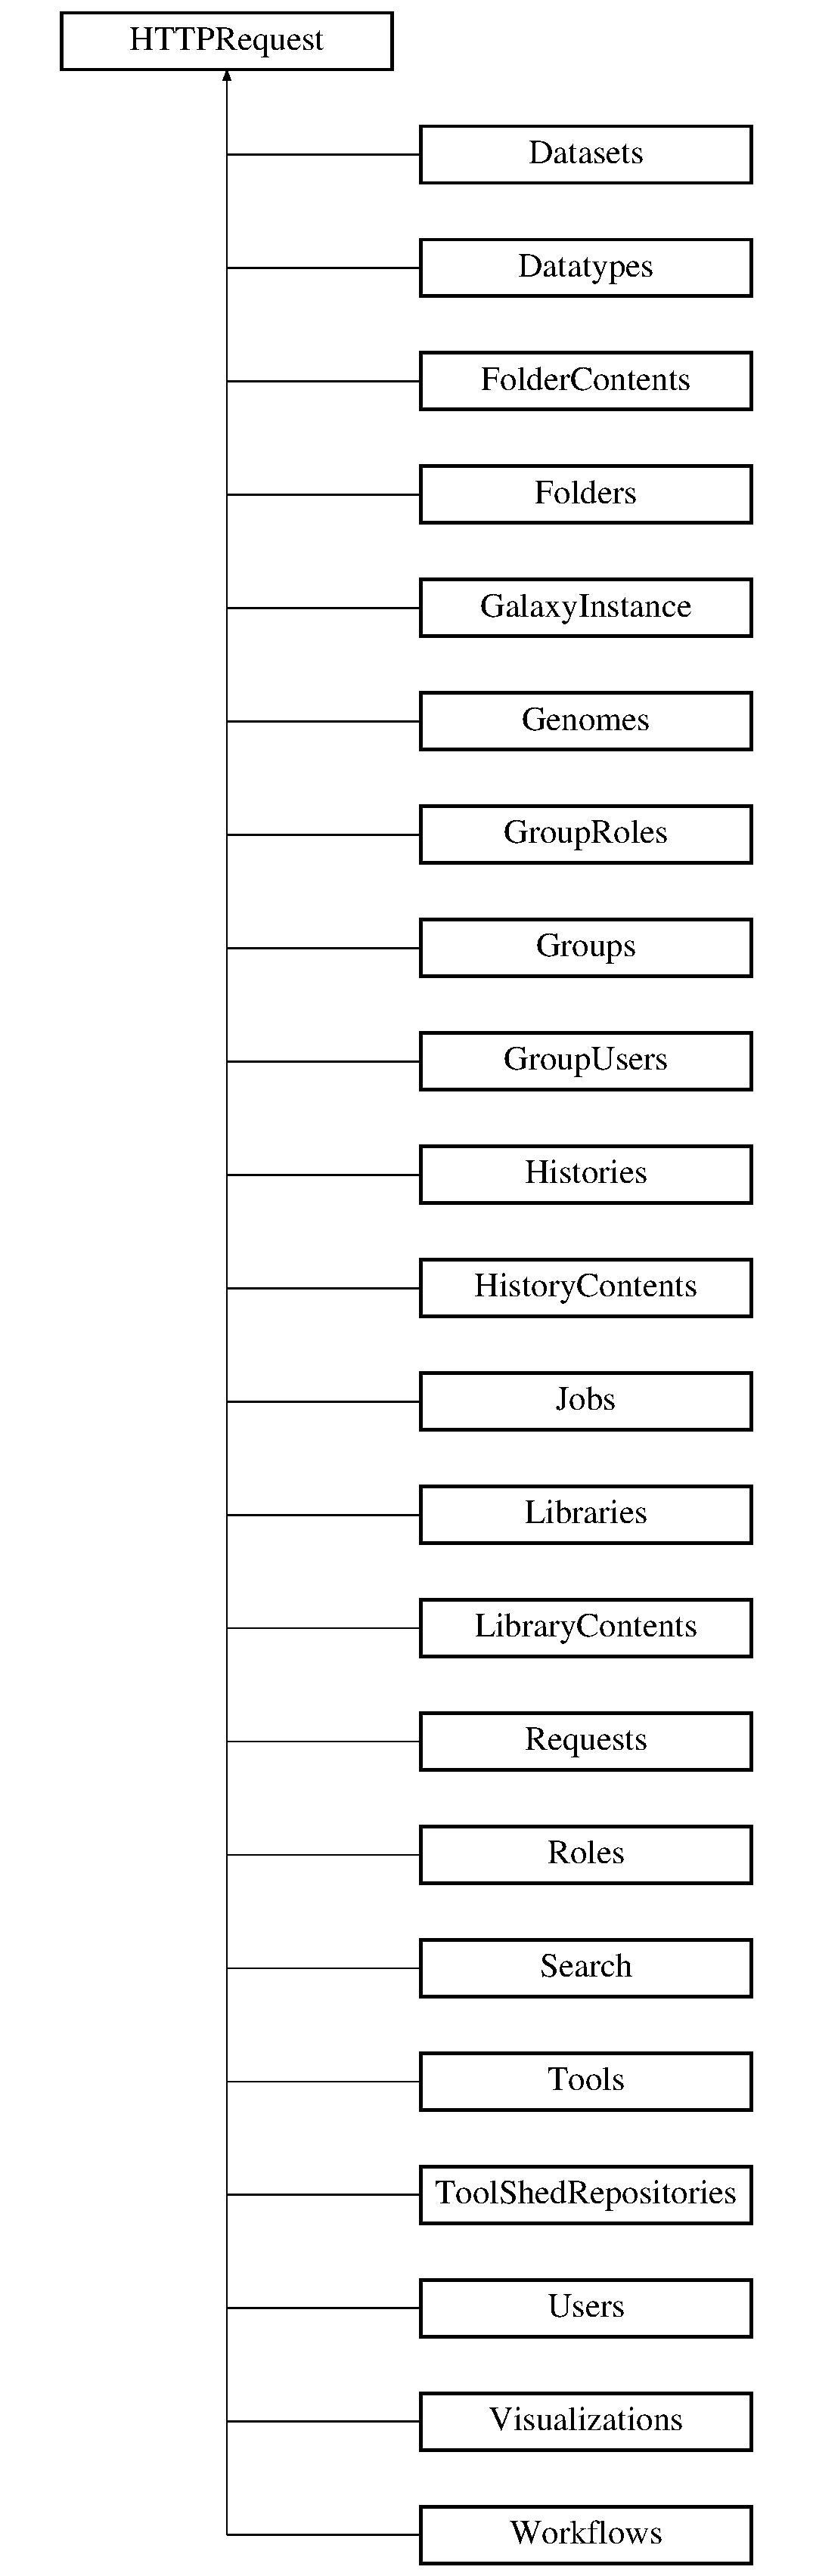
\includegraphics[height=12.000000cm]{classHTTPRequest}
\end{center}
\end{figure}
\subsection*{Public Member Functions}
\begin{DoxyCompactItemize}
\item 
\hyperlink{classHTTPRequest_a4e8d9f9045aec31421fe7a351a670192}{\+\_\+\+\_\+construct} ()
\item 
\hyperlink{classHTTPRequest_acdbc89e298a3ab5beb0a00f4c67646ad}{get\+Error} ()
\item 
\hyperlink{classHTTPRequest_a8e705d701b167a71861e53c329f12824}{get\+Error\+Message} ()
\item 
\hyperlink{classHTTPRequest_a876aad5c328ef5a71345a04ff697def5}{get\+Error\+Type} ()
\end{DoxyCompactItemize}
\subsection*{Protected Member Functions}
\begin{DoxyCompactItemize}
\item 
\hyperlink{classHTTPRequest_a99ceafd4438f0401b6c101753c7c3132}{http\+G\+ET} (\$U\+RL)
\item 
\hyperlink{classHTTPRequest_a7519cc4959bd359ef6d3749a0e430042}{http\+P\+O\+ST} (\$U\+RL, \$post\+\_\+fields=N\+U\+LL)
\item 
\hyperlink{classHTTPRequest_abbe45ffd58c968cf0dfd6de7c443bee5}{http\+P\+UT} (\$U\+RL, \$input=N\+U\+LL)
\item 
\hyperlink{classHTTPRequest_a6d34dd87ee714604d6d4aaa677d52729}{get\+Remote\+File} (\$U\+RL, \$file\+\_\+name)
\item 
\hyperlink{classHTTPRequest_a2a2d2264470fb233ae5e0878b021927e}{http\+D\+E\+L\+E\+TE} (\$U\+RL, \$input=N\+U\+LL)
\item 
\hyperlink{classHTTPRequest_a16855344f3ba37cb4247a5b9916798dd}{auth} (\$U\+RL, \$username, \$password)
\item 
\hyperlink{classHTTPRequest_a4f9c6fcfb8efb81c4ec2aa1861de7ef0}{set\+Error} (\$type, \$message)
\item 
\hyperlink{classHTTPRequest_a179b9f578b700fd35e4b31b448c824da}{expect\+Array} (\$response)
\end{DoxyCompactItemize}


\subsection{Constructor \& Destructor Documentation}
\index{H\+T\+T\+P\+Request@{H\+T\+T\+P\+Request}!\+\_\+\+\_\+construct@{\+\_\+\+\_\+construct}}
\index{\+\_\+\+\_\+construct@{\+\_\+\+\_\+construct}!H\+T\+T\+P\+Request@{H\+T\+T\+P\+Request}}
\subsubsection[{\texorpdfstring{\+\_\+\+\_\+construct()}{\_\_construct()}}]{\setlength{\rightskip}{0pt plus 5cm}H\+T\+T\+P\+Request\+::\+\_\+\+\_\+construct (
\begin{DoxyParamCaption}
{}
\end{DoxyParamCaption}
)}\hypertarget{classHTTPRequest_a4e8d9f9045aec31421fe7a351a670192}{}\label{classHTTPRequest_a4e8d9f9045aec31421fe7a351a670192}
The Rest Manager constructor.


\begin{DoxyParams}{Parameters}
{\em \hyperlink{classRequestError}{Request\+Error}} & requesterror Optional, set the class\textquotesingle{}s request error to a pre-\/existing \hyperlink{classRequestError}{Request\+Error}.\\
\hline
\end{DoxyParams}
\begin{DoxyReturn}{Returns}
An instance of a Rest\+Manager class. 
\end{DoxyReturn}


\subsection{Member Function Documentation}
\index{H\+T\+T\+P\+Request@{H\+T\+T\+P\+Request}!auth@{auth}}
\index{auth@{auth}!H\+T\+T\+P\+Request@{H\+T\+T\+P\+Request}}
\subsubsection[{\texorpdfstring{auth(\$\+U\+R\+L, \$username, \$password)}{auth($URL, $username, $password)}}]{\setlength{\rightskip}{0pt plus 5cm}H\+T\+T\+P\+Request\+::auth (
\begin{DoxyParamCaption}
\item[{}]{\$\+U\+RL, }
\item[{}]{\$username, }
\item[{}]{\$password}
\end{DoxyParamCaption}
)\hspace{0.3cm}{\ttfamily [protected]}}\hypertarget{classHTTPRequest_a16855344f3ba37cb4247a5b9916798dd}{}\label{classHTTPRequest_a16855344f3ba37cb4247a5b9916798dd}

\begin{DoxyParams}[1]{Parameters}
unknown & {\em \$\+U\+RL} & \\
\hline
unknown & {\em \$username} & \\
\hline
unknown & {\em \$password} & \\
\hline
\end{DoxyParams}
\index{H\+T\+T\+P\+Request@{H\+T\+T\+P\+Request}!expect\+Array@{expect\+Array}}
\index{expect\+Array@{expect\+Array}!H\+T\+T\+P\+Request@{H\+T\+T\+P\+Request}}
\subsubsection[{\texorpdfstring{expect\+Array(\$response)}{expectArray($response)}}]{\setlength{\rightskip}{0pt plus 5cm}H\+T\+T\+P\+Request\+::expect\+Array (
\begin{DoxyParamCaption}
\item[{}]{\$response}
\end{DoxyParamCaption}
)\hspace{0.3cm}{\ttfamily [protected]}}\hypertarget{classHTTPRequest_a179b9f578b700fd35e4b31b448c824da}{}\label{classHTTPRequest_a179b9f578b700fd35e4b31b448c824da}
Checks if the provided value is an array and sets an error if not.

This is a helper function to help children class deal with the case when Galaxy does not return a J\+S\+ON array as expected. Sometimes when there is an error the error message is returned in a J\+S\+ON array and can be handled by our get\+C\+U\+R\+L\+Response function. But otherwise that function can\textquotesingle{}t distinguish between a string that is returned and an error. So, this function allows children class to check that the response is an array if they expect that it should be.


\begin{DoxyParams}[1]{Parameters}
unknown & {\em \$response} & \\
\hline
\end{DoxyParams}
\index{H\+T\+T\+P\+Request@{H\+T\+T\+P\+Request}!get\+Error@{get\+Error}}
\index{get\+Error@{get\+Error}!H\+T\+T\+P\+Request@{H\+T\+T\+P\+Request}}
\subsubsection[{\texorpdfstring{get\+Error()}{getError()}}]{\setlength{\rightskip}{0pt plus 5cm}H\+T\+T\+P\+Request\+::get\+Error (
\begin{DoxyParamCaption}
{}
\end{DoxyParamCaption}
)}\hypertarget{classHTTPRequest_acdbc89e298a3ab5beb0a00f4c67646ad}{}\label{classHTTPRequest_acdbc89e298a3ab5beb0a00f4c67646ad}
\begin{DoxyReturn}{Returns}
string error message from the server or C\+U\+RL. 
\end{DoxyReturn}
\index{H\+T\+T\+P\+Request@{H\+T\+T\+P\+Request}!get\+Error\+Message@{get\+Error\+Message}}
\index{get\+Error\+Message@{get\+Error\+Message}!H\+T\+T\+P\+Request@{H\+T\+T\+P\+Request}}
\subsubsection[{\texorpdfstring{get\+Error\+Message()}{getErrorMessage()}}]{\setlength{\rightskip}{0pt plus 5cm}H\+T\+T\+P\+Request\+::get\+Error\+Message (
\begin{DoxyParamCaption}
{}
\end{DoxyParamCaption}
)}\hypertarget{classHTTPRequest_a8e705d701b167a71861e53c329f12824}{}\label{classHTTPRequest_a8e705d701b167a71861e53c329f12824}
\begin{DoxyReturn}{Returns}
The 
\end{DoxyReturn}
\index{H\+T\+T\+P\+Request@{H\+T\+T\+P\+Request}!get\+Error\+Type@{get\+Error\+Type}}
\index{get\+Error\+Type@{get\+Error\+Type}!H\+T\+T\+P\+Request@{H\+T\+T\+P\+Request}}
\subsubsection[{\texorpdfstring{get\+Error\+Type()}{getErrorType()}}]{\setlength{\rightskip}{0pt plus 5cm}H\+T\+T\+P\+Request\+::get\+Error\+Type (
\begin{DoxyParamCaption}
{}
\end{DoxyParamCaption}
)}\hypertarget{classHTTPRequest_a876aad5c328ef5a71345a04ff697def5}{}\label{classHTTPRequest_a876aad5c328ef5a71345a04ff697def5}
\begin{DoxyReturn}{Returns}
The 
\end{DoxyReturn}
\index{H\+T\+T\+P\+Request@{H\+T\+T\+P\+Request}!get\+Remote\+File@{get\+Remote\+File}}
\index{get\+Remote\+File@{get\+Remote\+File}!H\+T\+T\+P\+Request@{H\+T\+T\+P\+Request}}
\subsubsection[{\texorpdfstring{get\+Remote\+File(\$\+U\+R\+L, \$file\+\_\+name)}{getRemoteFile($URL, $file\_name)}}]{\setlength{\rightskip}{0pt plus 5cm}H\+T\+T\+P\+Request\+::get\+Remote\+File (
\begin{DoxyParamCaption}
\item[{}]{\$\+U\+RL, }
\item[{}]{\$file\+\_\+name}
\end{DoxyParamCaption}
)\hspace{0.3cm}{\ttfamily [protected]}}\hypertarget{classHTTPRequest_a6d34dd87ee714604d6d4aaa677d52729}{}\label{classHTTPRequest_a6d34dd87ee714604d6d4aaa677d52729}

\begin{DoxyParams}{Parameters}
{\em \$\+U\+RL} & \\
\hline
{\em \$file\+\_\+name} & \\
\hline
\end{DoxyParams}
\begin{DoxyReturn}{Returns}

\end{DoxyReturn}
\index{H\+T\+T\+P\+Request@{H\+T\+T\+P\+Request}!http\+D\+E\+L\+E\+TE@{http\+D\+E\+L\+E\+TE}}
\index{http\+D\+E\+L\+E\+TE@{http\+D\+E\+L\+E\+TE}!H\+T\+T\+P\+Request@{H\+T\+T\+P\+Request}}
\subsubsection[{\texorpdfstring{http\+D\+E\+L\+E\+T\+E(\$\+U\+R\+L, \$input=\+N\+U\+L\+L)}{httpDELETE($URL, $input=NULL)}}]{\setlength{\rightskip}{0pt plus 5cm}H\+T\+T\+P\+Request\+::http\+D\+E\+L\+E\+TE (
\begin{DoxyParamCaption}
\item[{}]{\$\+U\+RL, }
\item[{}]{\$input = {\ttfamily NULL}}
\end{DoxyParamCaption}
)\hspace{0.3cm}{\ttfamily [protected]}}\hypertarget{classHTTPRequest_a2a2d2264470fb233ae5e0878b021927e}{}\label{classHTTPRequest_a2a2d2264470fb233ae5e0878b021927e}
Universal D\+E\+L\+E\+TE request


\begin{DoxyParams}{Parameters}
{\em \$input} & The input data to give to the url. \\
\hline
{\em \$\+U\+RL} & The path to perform the D\+E\+L\+E\+TE request.\\
\hline
\end{DoxyParams}
\begin{DoxyReturn}{Returns}
curl server response 
\end{DoxyReturn}
\index{H\+T\+T\+P\+Request@{H\+T\+T\+P\+Request}!http\+G\+ET@{http\+G\+ET}}
\index{http\+G\+ET@{http\+G\+ET}!H\+T\+T\+P\+Request@{H\+T\+T\+P\+Request}}
\subsubsection[{\texorpdfstring{http\+G\+E\+T(\$\+U\+R\+L)}{httpGET($URL)}}]{\setlength{\rightskip}{0pt plus 5cm}H\+T\+T\+P\+Request\+::http\+G\+ET (
\begin{DoxyParamCaption}
\item[{}]{\$\+U\+RL}
\end{DoxyParamCaption}
)\hspace{0.3cm}{\ttfamily [protected]}}\hypertarget{classHTTPRequest_a99ceafd4438f0401b6c101753c7c3132}{}\label{classHTTPRequest_a99ceafd4438f0401b6c101753c7c3132}
Performs a G\+ET request.


\begin{DoxyParams}{Parameters}
{\em url} & The U\+RL to perform the G\+ET request on.\\
\hline
\end{DoxyParams}
\begin{DoxyReturn}{Returns}
curl server response. 
\end{DoxyReturn}
\index{H\+T\+T\+P\+Request@{H\+T\+T\+P\+Request}!http\+P\+O\+ST@{http\+P\+O\+ST}}
\index{http\+P\+O\+ST@{http\+P\+O\+ST}!H\+T\+T\+P\+Request@{H\+T\+T\+P\+Request}}
\subsubsection[{\texorpdfstring{http\+P\+O\+S\+T(\$\+U\+R\+L, \$post\+\_\+fields=\+N\+U\+L\+L)}{httpPOST($URL, $post\_fields=NULL)}}]{\setlength{\rightskip}{0pt plus 5cm}H\+T\+T\+P\+Request\+::http\+P\+O\+ST (
\begin{DoxyParamCaption}
\item[{}]{\$\+U\+RL, }
\item[{}]{\$post\+\_\+fields = {\ttfamily NULL}}
\end{DoxyParamCaption}
)\hspace{0.3cm}{\ttfamily [protected]}}\hypertarget{classHTTPRequest_a7519cc4959bd359ef6d3749a0e430042}{}\label{classHTTPRequest_a7519cc4959bd359ef6d3749a0e430042}
Perform a P\+O\+ST request.


\begin{DoxyParams}{Parameters}
{\em U\+RL} & The url to perform the P\+O\+ST request on. \\
\hline
{\em Input} & The input data to a given U\+RL.\\
\hline
\end{DoxyParams}
\begin{DoxyReturn}{Returns}
curl server response. 
\end{DoxyReturn}
\index{H\+T\+T\+P\+Request@{H\+T\+T\+P\+Request}!http\+P\+UT@{http\+P\+UT}}
\index{http\+P\+UT@{http\+P\+UT}!H\+T\+T\+P\+Request@{H\+T\+T\+P\+Request}}
\subsubsection[{\texorpdfstring{http\+P\+U\+T(\$\+U\+R\+L, \$input=\+N\+U\+L\+L)}{httpPUT($URL, $input=NULL)}}]{\setlength{\rightskip}{0pt plus 5cm}H\+T\+T\+P\+Request\+::http\+P\+UT (
\begin{DoxyParamCaption}
\item[{}]{\$\+U\+RL, }
\item[{}]{\$input = {\ttfamily NULL}}
\end{DoxyParamCaption}
)\hspace{0.3cm}{\ttfamily [protected]}}\hypertarget{classHTTPRequest_abbe45ffd58c968cf0dfd6de7c443bee5}{}\label{classHTTPRequest_abbe45ffd58c968cf0dfd6de7c443bee5}
Perform a P\+UT request


\begin{DoxyParams}{Parameters}
{\em U\+RL} & The U\+RL to perform the P\+UT request on. \\
\hline
{\em Input} & The input data to give to the U\+RL.\\
\hline
\end{DoxyParams}
\begin{DoxyReturn}{Returns}
curl server response. 
\end{DoxyReturn}
\index{H\+T\+T\+P\+Request@{H\+T\+T\+P\+Request}!set\+Error@{set\+Error}}
\index{set\+Error@{set\+Error}!H\+T\+T\+P\+Request@{H\+T\+T\+P\+Request}}
\subsubsection[{\texorpdfstring{set\+Error(\$type, \$message)}{setError($type, $message)}}]{\setlength{\rightskip}{0pt plus 5cm}H\+T\+T\+P\+Request\+::set\+Error (
\begin{DoxyParamCaption}
\item[{}]{\$type, }
\item[{}]{\$message}
\end{DoxyParamCaption}
)\hspace{0.3cm}{\ttfamily [protected]}}\hypertarget{classHTTPRequest_a4f9c6fcfb8efb81c4ec2aa1861de7ef0}{}\label{classHTTPRequest_a4f9c6fcfb8efb81c4ec2aa1861de7ef0}

\begin{DoxyParams}{Parameters}
{\em \$type} & \\
\hline
{\em \$message} & \\
\hline
\end{DoxyParams}


The documentation for this class was generated from the following file\+:\begin{DoxyCompactItemize}
\item 
\hyperlink{HTTPRequest_8inc}{H\+T\+T\+P\+Request.\+inc}\end{DoxyCompactItemize}

\hypertarget{classJobs}{}\section{Jobs Class Reference}
\label{classJobs}\index{Jobs@{Jobs}}
Inheritance diagram for Jobs\+:\begin{figure}[H]
\begin{center}
\leavevmode
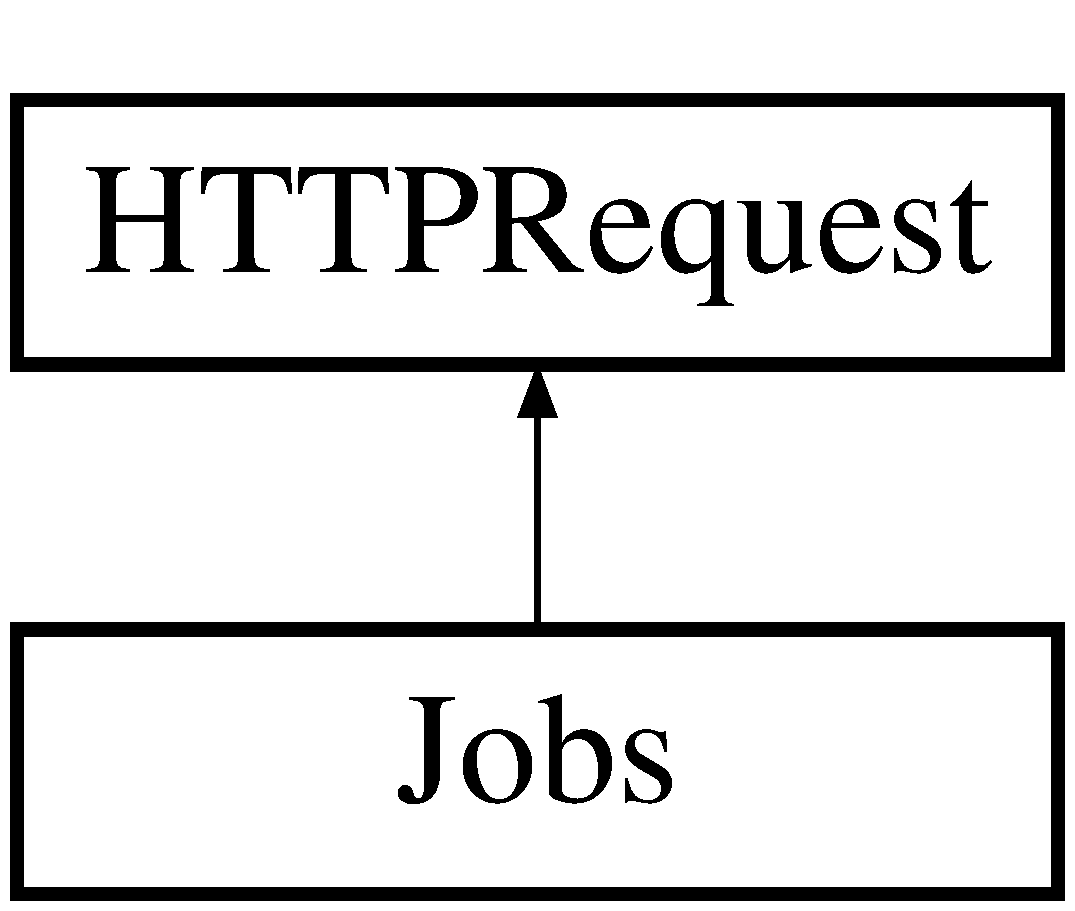
\includegraphics[height=2.000000cm]{classJobs}
\end{center}
\end{figure}
\subsection*{Public Member Functions}
\begin{DoxyCompactItemize}
\item 
\hyperlink{classJobs_ad7a85851751aa89c92294c55aa9fcc87}{\+\_\+\+\_\+construct} (\$galaxy)
\item 
\hyperlink{classJobs_abadc1a5ebccaeb6b5b977328609f5a34}{build\+For\+Rerun} (\$job\+\_\+id)
\item 
\hyperlink{classJobs_a4859adf323104d74772c2d9cbcb04331}{inputs} (\$job\+\_\+id)
\item 
\hyperlink{classJobs_a6fa75d976f7dcbe31cb1191effa0a9ea}{outputs} (\$job\+\_\+id)
\item 
\hyperlink{classJobs_af95758c7cad6b00529344f0ddeb1e830}{show} (\$job\+\_\+id)
\item 
\hyperlink{classJobs_a428dddc2ccac56c7e3c83f524d9f719c}{index} (\$state=N\+U\+LL, \$tool\+\_\+ids=N\+U\+LL, \$date\+\_\+range\+\_\+min=N\+U\+LL, \$date\+\_\+range\+\_\+max=N\+U\+LL, \$history\+\_\+id=N\+U\+LL)
\item 
\hyperlink{classJobs_a4707d2d193d37086cbac02f9c7463eab}{create} ()
\item 
\hyperlink{classJobs_a0f7e6dedeee443ad8c262ee4d55df136}{search} (\$params)
\end{DoxyCompactItemize}
\subsection*{Additional Inherited Members}


\subsection{Constructor \& Destructor Documentation}
\index{Jobs@{Jobs}!\+\_\+\+\_\+construct@{\+\_\+\+\_\+construct}}
\index{\+\_\+\+\_\+construct@{\+\_\+\+\_\+construct}!Jobs@{Jobs}}
\subsubsection[{\texorpdfstring{\+\_\+\+\_\+construct(\$galaxy)}{\_\_construct($galaxy)}}]{\setlength{\rightskip}{0pt plus 5cm}Jobs\+::\+\_\+\+\_\+construct (
\begin{DoxyParamCaption}
\item[{}]{\$galaxy}
\end{DoxyParamCaption}
)}\hypertarget{classJobs_ad7a85851751aa89c92294c55aa9fcc87}{}\label{classJobs_ad7a85851751aa89c92294c55aa9fcc87}
The \hyperlink{classJobs}{Jobs} constructor.


\begin{DoxyParams}[1]{Parameters}
\hyperlink{classGalaxyInstance}{Galaxy\+Instance} & {\em \$galaxy} & A \hyperlink{classGalaxyInstance}{Galaxy\+Instance} object.\\
\hline
\end{DoxyParams}
\begin{DoxyReturn}{Returns}
An instance of a \hyperlink{classJobs}{Jobs} object. 
\end{DoxyReturn}


\subsection{Member Function Documentation}
\index{Jobs@{Jobs}!build\+For\+Rerun@{build\+For\+Rerun}}
\index{build\+For\+Rerun@{build\+For\+Rerun}!Jobs@{Jobs}}
\subsubsection[{\texorpdfstring{build\+For\+Rerun(\$job\+\_\+id)}{buildForRerun($job\_id)}}]{\setlength{\rightskip}{0pt plus 5cm}Jobs\+::build\+For\+Rerun (
\begin{DoxyParamCaption}
\item[{}]{\$job\+\_\+id}
\end{DoxyParamCaption}
)}\hypertarget{classJobs_abadc1a5ebccaeb6b5b977328609f5a34}{}\label{classJobs_abadc1a5ebccaeb6b5b977328609f5a34}
Retreive a tool input template populated with this job\textquotesingle{}s information.

Corresponds to the Galaxy Api/path at\+: G\+ET /api/jobs/\{encoded\+\_\+job\+\_\+id\}/build\+\_\+for\+\_\+rerun This function is suitable for rerunning or rendering parameters of the job.


\begin{DoxyParams}{Parameters}
{\em job} & id The job id of the job whose information to retreive. The job id can be ontained from this class\textquotesingle{}s \hyperlink{classJobs_a428dddc2ccac56c7e3c83f524d9f719c}{index()} function.\\
\hline
\end{DoxyParams}
\begin{DoxyReturn}{Returns}
An array containing ouput informaiton of the tool that has been built. 
\end{DoxyReturn}
\index{Jobs@{Jobs}!create@{create}}
\index{create@{create}!Jobs@{Jobs}}
\subsubsection[{\texorpdfstring{create()}{create()}}]{\setlength{\rightskip}{0pt plus 5cm}Jobs\+::create (
\begin{DoxyParamCaption}
{}
\end{DoxyParamCaption}
)}\hypertarget{classJobs_a4707d2d193d37086cbac02f9c7463eab}{}\label{classJobs_a4707d2d193d37086cbac02f9c7463eab}
This function is not implemented by its python counterpart

N\+O\+TE\+: Creating/submitting a job is actually run under tools.\+py in the Galaxy api

\begin{DoxyReturn}{Returns}
F\+A\+L\+SE 
\end{DoxyReturn}
\index{Jobs@{Jobs}!index@{index}}
\index{index@{index}!Jobs@{Jobs}}
\subsubsection[{\texorpdfstring{index(\$state=\+N\+U\+L\+L, \$tool\+\_\+ids=\+N\+U\+L\+L, \$date\+\_\+range\+\_\+min=\+N\+U\+L\+L, \$date\+\_\+range\+\_\+max=\+N\+U\+L\+L, \$history\+\_\+id=\+N\+U\+L\+L)}{index($state=NULL, $tool\_ids=NULL, $date\_range\_min=NULL, $date\_range\_max=NULL, $history\_id=NULL)}}]{\setlength{\rightskip}{0pt plus 5cm}Jobs\+::index (
\begin{DoxyParamCaption}
\item[{}]{\$state = {\ttfamily NULL}, }
\item[{}]{\$tool\+\_\+ids = {\ttfamily NULL}, }
\item[{}]{\$date\+\_\+range\+\_\+min = {\ttfamily NULL}, }
\item[{}]{\$date\+\_\+range\+\_\+max = {\ttfamily NULL}, }
\item[{}]{\$history\+\_\+id = {\ttfamily NULL}}
\end{DoxyParamCaption}
)}\hypertarget{classJobs_a428dddc2ccac56c7e3c83f524d9f719c}{}\label{classJobs_a428dddc2ccac56c7e3c83f524d9f719c}
Retreive a list of jobs for current user.

Corresponds to the Galaxy Api method/path\+: G\+ET /api/jobs


\begin{DoxyParams}{Parameters}
{\em state} & filter job search by any one of these conditions\+: \textquotesingle{}new\textquotesingle{}, \textquotesingle{}upload\textquotesingle{}, \textquotesingle{}waiting\textquotesingle{}, \textquotesingle{}queued\textquotesingle{}, \textquotesingle{}running\textquotesingle{}, \textquotesingle{}ok\textquotesingle{}, \textquotesingle{}error\textquotesingle{}, \textquotesingle{}paused\textquotesingle{}, \textquotesingle{}deleted\textquotesingle{}, \textquotesingle{}deleted\+\_\+now\textquotesingle{} \\
\hline
{\em tool\+\_\+ids.} & A list of tool ids that limit the search to include only those with given tool\+\_\+ids. To find tool id\textquotesingle{}s, please refer to this class\textquotesingle{}s \hyperlink{classJobs_a428dddc2ccac56c7e3c83f524d9f719c}{index()} function. \\
\hline
{\em date\+\_\+range\+\_\+min} & Limit the search of jobs updated after this date. \\
\hline
{\em date\+\_\+range\+\_\+max} & Limit the search of jobs updated before this date. \\
\hline
{\em history\+\_\+id} & Limit listing of jobs to those that match history\+\_\+id. To find the history id, please refer to the history class.\\
\hline
\end{DoxyParams}
\begin{DoxyReturn}{Returns}
An array containing a list of all the jobs that matched the given parameters. 
\end{DoxyReturn}
\index{Jobs@{Jobs}!inputs@{inputs}}
\index{inputs@{inputs}!Jobs@{Jobs}}
\subsubsection[{\texorpdfstring{inputs(\$job\+\_\+id)}{inputs($job\_id)}}]{\setlength{\rightskip}{0pt plus 5cm}Jobs\+::inputs (
\begin{DoxyParamCaption}
\item[{}]{\$job\+\_\+id}
\end{DoxyParamCaption}
)}\hypertarget{classJobs_a4859adf323104d74772c2d9cbcb04331}{}\label{classJobs_a4859adf323104d74772c2d9cbcb04331}
Retreive the input datasets created from the specified job.

Corresponds to the Galaxy Api/path at\+: G\+E\+T/api/jobs/\{encoded\+\_\+job\+\_\+id\}/inputs


\begin{DoxyParams}{Parameters}
{\em job\+\_\+id} & The job id of the job whose information to retreive. The job id can be ontained from this class\textquotesingle{}s \hyperlink{classJobs_a428dddc2ccac56c7e3c83f524d9f719c}{index()} function.\\
\hline
\end{DoxyParams}
\begin{DoxyReturn}{Returns}
An array containing ouput informaiton of the job input. 
\end{DoxyReturn}
\index{Jobs@{Jobs}!outputs@{outputs}}
\index{outputs@{outputs}!Jobs@{Jobs}}
\subsubsection[{\texorpdfstring{outputs(\$job\+\_\+id)}{outputs($job\_id)}}]{\setlength{\rightskip}{0pt plus 5cm}Jobs\+::outputs (
\begin{DoxyParamCaption}
\item[{}]{\$job\+\_\+id}
\end{DoxyParamCaption}
)}\hypertarget{classJobs_a6fa75d976f7dcbe31cb1191effa0a9ea}{}\label{classJobs_a6fa75d976f7dcbe31cb1191effa0a9ea}
Retreive the output datasets created from the specified job.

Corresponds to the Galaxy Api/path at\+: G\+E\+T/api/jobs/\{encoded\+\_\+job\+\_\+id\}/inputs.


\begin{DoxyParams}{Parameters}
{\em job\+\_\+id} & The job id of the job whose information to retreive. The job id can be ontained from this class\textquotesingle{}s \hyperlink{classJobs_a428dddc2ccac56c7e3c83f524d9f719c}{index()} function.\\
\hline
\end{DoxyParams}
\begin{DoxyReturn}{Returns}
An array containing ouput informaiton of the job outputs. 
\end{DoxyReturn}
\index{Jobs@{Jobs}!search@{search}}
\index{search@{search}!Jobs@{Jobs}}
\subsubsection[{\texorpdfstring{search(\$params)}{search($params)}}]{\setlength{\rightskip}{0pt plus 5cm}Jobs\+::search (
\begin{DoxyParamCaption}
\item[{}]{\$params}
\end{DoxyParamCaption}
)}\hypertarget{classJobs_a0f7e6dedeee443ad8c262ee4d55df136}{}\label{classJobs_a0f7e6dedeee443ad8c262ee4d55df136}
\hyperlink{classSearch}{Search} for previously created jobs.

Corresponds to the Galaxy api/path at\+: P\+O\+ST /api/jobs/search

This method is designed to scan the list of previously run jobs and find records of jobs that had the exact some input parameters and datasets. This can be used to minimize, the amount of repeated work, and simplyrecycle the old results.


\begin{DoxyParams}{Parameters}
{\em \$params} & A key value (associative array) where the keys can be the following\+:
\begin{DoxyItemize}
\item tool\+\_\+id\+: Required. The tool id to execute. To find the tool id, use the index function of this class.
\item inputs\+: Required. An associative array of key/value pairs where valid keys are \textquotesingle{}id\textquotesingle{} and \textquotesingle{}src\textquotesingle{} and \textquotesingle{}id\textquotesingle{} is a tool\+\_\+id (e.\+g. wc\+\_\+gnu), and \textquotesingle{}src\textquotesingle{} is is optional but defaults to \textquotesingle{}hda\textquotesingle{}. Alternatively, if multiple inputs are desired, this can be an array of associative arrays.
\item state\+: Optional. The state of the job\+: \textquotesingle{}running\textquotesingle{}, \textquotesingle{}queued\textquotesingle{}, \textquotesingle{}waiting\textquotesingle{}, \textquotesingle{}ok\textquotesingle{}. 
\end{DoxyItemize}\\
\hline
\end{DoxyParams}
\begin{DoxyReturn}{Returns}
An array of jobs matching the provided arguments. 
\end{DoxyReturn}
\index{Jobs@{Jobs}!show@{show}}
\index{show@{show}!Jobs@{Jobs}}
\subsubsection[{\texorpdfstring{show(\$job\+\_\+id)}{show($job\_id)}}]{\setlength{\rightskip}{0pt plus 5cm}Jobs\+::show (
\begin{DoxyParamCaption}
\item[{}]{\$job\+\_\+id}
\end{DoxyParamCaption}
)}\hypertarget{classJobs_af95758c7cad6b00529344f0ddeb1e830}{}\label{classJobs_af95758c7cad6b00529344f0ddeb1e830}
Retreive information about a specific job

Corresponds to the Galaxy A\+PI function/path\+: G\+ET /api/jobs/\{folder\+\_\+id\}


\begin{DoxyParams}{Parameters}
{\em \$folder\+\_\+id} & The folder that you would like to see. Please see the \hyperlink{classJobs_a428dddc2ccac56c7e3c83f524d9f719c}{index()} function in this class to obtain folder ids.\\
\hline
\end{DoxyParams}
\begin{DoxyReturn}{Returns}
J\+S\+ON array containing information about the specified job. 
\end{DoxyReturn}


The documentation for this class was generated from the following file\+:\begin{DoxyCompactItemize}
\item 
\hyperlink{Jobs_8inc}{Jobs.\+inc}\end{DoxyCompactItemize}

\hypertarget{classLibraries}{}\section{Libraries Class Reference}
\label{classLibraries}\index{Libraries@{Libraries}}
Inheritance diagram for Libraries\+:\begin{figure}[H]
\begin{center}
\leavevmode
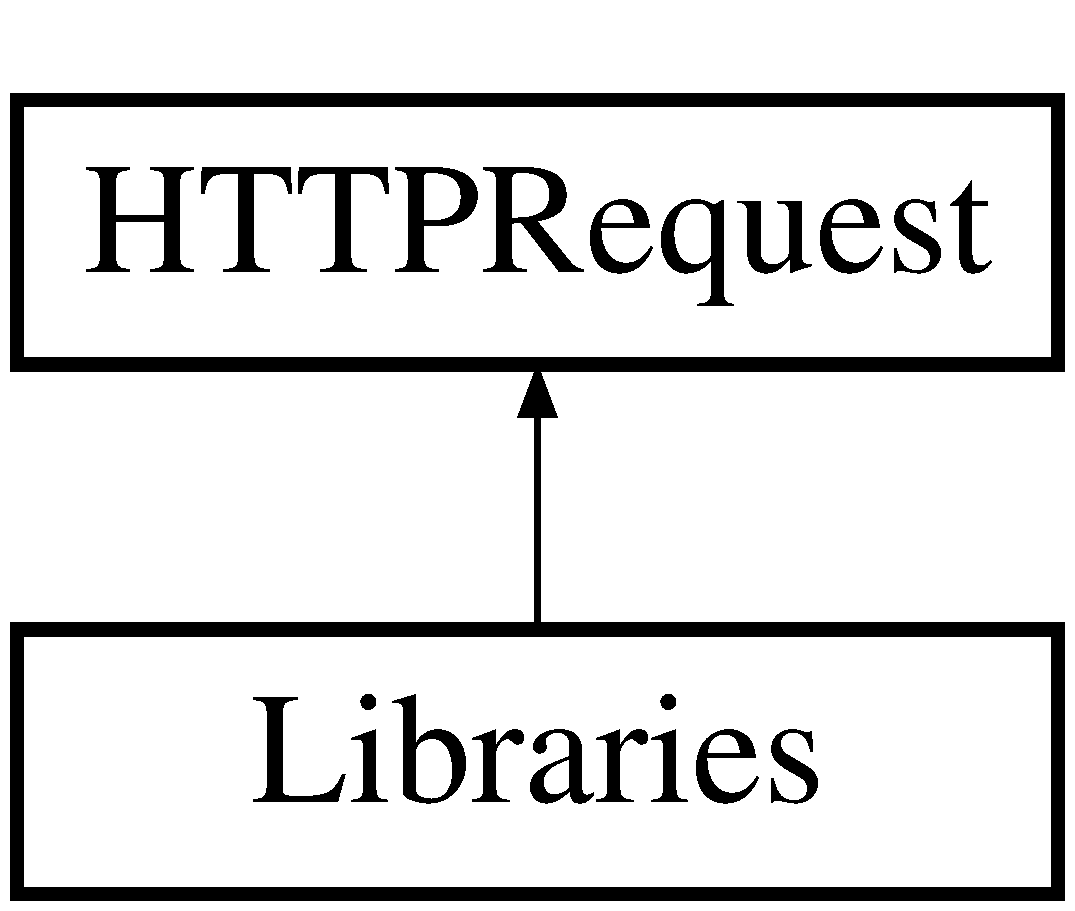
\includegraphics[height=2.000000cm]{classLibraries}
\end{center}
\end{figure}
\subsection*{Public Member Functions}
\begin{DoxyCompactItemize}
\item 
\hyperlink{classLibraries_a84aba8841f094815b3af6e4affed79c0}{\+\_\+\+\_\+construct} (\$galaxy)
\item 
\hyperlink{classLibraries_a5090fa7a9be0e26a91590d651a32abe9}{create} (\$name, \$description=N\+U\+LL, \$synopsis=N\+U\+LL)
\item 
\hyperlink{classLibraries_a66d9b028c4fde6edef8e3b7e0582d884}{update} (\$name, \$description=N\+U\+LL, \$synopsis=N\+U\+LL)
\item 
\hyperlink{classLibraries_a93ffa5a990c77a0872a3adb2f0a69158}{index} (\$deleted=F\+A\+L\+SE)
\item 
\hyperlink{classLibraries_a8310b5f58da502f256e87b8d42915454}{show} (\$library\+\_\+id, \$deleted=F\+A\+L\+SE)
\item 
\hyperlink{classLibraries_a3de3c2fdbaa21d621ad6fd7bb4f83a49}{delete} (\$library\+\_\+id, \$undelete=F\+A\+L\+SE)
\item 
\hyperlink{classLibraries_abad2211e5699eb1c296db1ac22bf478c}{get\+Permissions} (\$library\+\_\+id, \$scope=\textquotesingle{}available\textquotesingle{}, \$is\+\_\+library\+\_\+access=true)
\item 
\hyperlink{classLibraries_aea282014c5f7a983977c2b920885e798}{set\+Permissions} (\$library\+\_\+id, \$action=\textquotesingle{}set\+\_\+permissions\textquotesingle{}, \$access\+\_\+ids=array(), \$add\+\_\+ids=array(), \$manage\+\_\+ids=array(), \$modify\+\_\+ids=array())
\end{DoxyCompactItemize}
\subsection*{Additional Inherited Members}


\subsection{Constructor \& Destructor Documentation}
\index{Libraries@{Libraries}!\+\_\+\+\_\+construct@{\+\_\+\+\_\+construct}}
\index{\+\_\+\+\_\+construct@{\+\_\+\+\_\+construct}!Libraries@{Libraries}}
\subsubsection[{\texorpdfstring{\+\_\+\+\_\+construct(\$galaxy)}{\_\_construct($galaxy)}}]{\setlength{\rightskip}{0pt plus 5cm}Libraries\+::\+\_\+\+\_\+construct (
\begin{DoxyParamCaption}
\item[{}]{\$galaxy}
\end{DoxyParamCaption}
)}\hypertarget{classLibraries_a84aba8841f094815b3af6e4affed79c0}{}\label{classLibraries_a84aba8841f094815b3af6e4affed79c0}
The \hyperlink{classFolders}{Folders} constructor.


\begin{DoxyParams}[1]{Parameters}
\hyperlink{classGalaxyInstance}{Galaxy\+Instance} & {\em \$galaxy} & A \hyperlink{classGalaxyInstance}{Galaxy\+Instance} object.\\
\hline
\end{DoxyParams}
\begin{DoxyReturn}{Returns}
An instance of a \hyperlink{classLibraries}{Libraries} object. 
\end{DoxyReturn}


\subsection{Member Function Documentation}
\index{Libraries@{Libraries}!create@{create}}
\index{create@{create}!Libraries@{Libraries}}
\subsubsection[{\texorpdfstring{create(\$name, \$description=\+N\+U\+L\+L, \$synopsis=\+N\+U\+L\+L)}{create($name, $description=NULL, $synopsis=NULL)}}]{\setlength{\rightskip}{0pt plus 5cm}Libraries\+::create (
\begin{DoxyParamCaption}
\item[{}]{\$name, }
\item[{}]{\$description = {\ttfamily NULL}, }
\item[{}]{\$synopsis = {\ttfamily NULL}}
\end{DoxyParamCaption}
)}\hypertarget{classLibraries_a5090fa7a9be0e26a91590d651a32abe9}{}\label{classLibraries_a5090fa7a9be0e26a91590d651a32abe9}
Creates a new library.

Corresponds to the Galaxy Api/path\+: P\+O\+ST /api/libraries\+:


\begin{DoxyParams}{Parameters}
{\em Name} & The new library\textquotesingle{}s name. \\
\hline
{\em description\textquotesingle{}} & Optional the new library\textquotesingle{}s description. \\
\hline
{\em synopsis} & Otional a string containing a synopsis.\\
\hline
\end{DoxyParams}
\begin{DoxyReturn}{Returns}
An array containing the new library created. 
\end{DoxyReturn}
\index{Libraries@{Libraries}!delete@{delete}}
\index{delete@{delete}!Libraries@{Libraries}}
\subsubsection[{\texorpdfstring{delete(\$library\+\_\+id, \$undelete=\+F\+A\+L\+S\+E)}{delete($library\_id, $undelete=FALSE)}}]{\setlength{\rightskip}{0pt plus 5cm}Libraries\+::delete (
\begin{DoxyParamCaption}
\item[{}]{\$library\+\_\+id, }
\item[{}]{\$undelete = {\ttfamily FALSE}}
\end{DoxyParamCaption}
)}\hypertarget{classLibraries_a3de3c2fdbaa21d621ad6fd7bb4f83a49}{}\label{classLibraries_a3de3c2fdbaa21d621ad6fd7bb4f83a49}
Marks a specific library as deleted or a deleted library as not-\/deleted.

Corresponds to the Galaxy Api/path at D\+E\+L\+E\+TE /api/libraries/\{encoded\+\_\+id\}


\begin{DoxyParams}{Parameters}
{\em \$library\+\_\+id} & The id of the library to delete or undelete, to obtain library id\textquotesingle{}s please use this class\textquotesingle{}s \hyperlink{classLibraries_a93ffa5a990c77a0872a3adb2f0a69158}{index()} function. \\
\hline
{\em undelete} & If T\+R\+UE, the library will be undeleted if it is already deleted.\\
\hline
\end{DoxyParams}
\begin{DoxyReturn}{Returns}
An array containing details of the deleted or undeleted library. 
\end{DoxyReturn}
\index{Libraries@{Libraries}!get\+Permissions@{get\+Permissions}}
\index{get\+Permissions@{get\+Permissions}!Libraries@{Libraries}}
\subsubsection[{\texorpdfstring{get\+Permissions(\$library\+\_\+id, \$scope=\textquotesingle{}available\textquotesingle{}, \$is\+\_\+library\+\_\+access=true)}{getPermissions($library\_id, $scope='available', $is\_library\_access=true)}}]{\setlength{\rightskip}{0pt plus 5cm}Libraries\+::get\+Permissions (
\begin{DoxyParamCaption}
\item[{}]{\$library\+\_\+id, }
\item[{}]{\$scope = {\ttfamily \textquotesingle{}available\textquotesingle{}}, }
\item[{}]{\$is\+\_\+library\+\_\+access = {\ttfamily true}}
\end{DoxyParamCaption}
)}\hypertarget{classLibraries_abad2211e5699eb1c296db1ac22bf478c}{}\label{classLibraries_abad2211e5699eb1c296db1ac22bf478c}
Retreives the permission details for a given library.

Corresponds to the Galaxy A\+P\+I/path G\+ET /api/libraries/\{encoded\+\_\+library\+\_\+id\}/permissions


\begin{DoxyParams}{Parameters}
{\em library\+\_\+id} & The if of the library to receive permissions for. To obtain library id\textquotesingle{}s please use this class\textquotesingle{}s index function . $\ast$ \\
\hline
{\em scope} & The scope of the permission, either \textquotesingle{}available\textquotesingle{} or \textquotesingle{}current\textquotesingle{}. \\
\hline
{\em is\+\_\+library\+\_\+access} & If false, the function will not look for libraries with user access.\\
\hline
\end{DoxyParams}
\begin{DoxyReturn}{Returns}
An array containing details of the permissions of all libraries. 
\end{DoxyReturn}
\index{Libraries@{Libraries}!index@{index}}
\index{index@{index}!Libraries@{Libraries}}
\subsubsection[{\texorpdfstring{index(\$deleted=\+F\+A\+L\+S\+E)}{index($deleted=FALSE)}}]{\setlength{\rightskip}{0pt plus 5cm}Libraries\+::index (
\begin{DoxyParamCaption}
\item[{}]{\$deleted = {\ttfamily FALSE}}
\end{DoxyParamCaption}
)}\hypertarget{classLibraries_a93ffa5a990c77a0872a3adb2f0a69158}{}\label{classLibraries_a93ffa5a990c77a0872a3adb2f0a69158}
Retreives a list of summary data for all libraries.

Corresponds to the Galaxy Api/path\+: G\+ET /api/libraries


\begin{DoxyParams}{Parameters}
{\em deleted} & if T\+R\+UE, show only deleted libraries, if F\+A\+L\+SE show only non-\/deleted.\\
\hline
\end{DoxyParams}
\begin{DoxyReturn}{Returns}
An array of all of libraries. And all of the deleted libraries if appropriate. 
\end{DoxyReturn}
\index{Libraries@{Libraries}!set\+Permissions@{set\+Permissions}}
\index{set\+Permissions@{set\+Permissions}!Libraries@{Libraries}}
\subsubsection[{\texorpdfstring{set\+Permissions(\$library\+\_\+id, \$action=\textquotesingle{}set\+\_\+permissions\textquotesingle{}, \$access\+\_\+ids=array(), \$add\+\_\+ids=array(), \$manage\+\_\+ids=array(), \$modify\+\_\+ids=array())}{setPermissions($library\_id, $action='set\_permissions', $access\_ids=array(), $add\_ids=array(), $manage\_ids=array(), $modify\_ids=array())}}]{\setlength{\rightskip}{0pt plus 5cm}Libraries\+::set\+Permissions (
\begin{DoxyParamCaption}
\item[{}]{\$library\+\_\+id, }
\item[{}]{\$action = {\ttfamily \textquotesingle{}set\+\_\+permissions\textquotesingle{}}, }
\item[{}]{\$access\+\_\+ids = {\ttfamily array()}, }
\item[{}]{\$add\+\_\+ids = {\ttfamily array()}, }
\item[{}]{\$manage\+\_\+ids = {\ttfamily array()}, }
\item[{}]{\$modify\+\_\+ids = {\ttfamily array()}}
\end{DoxyParamCaption}
)}\hypertarget{classLibraries_aea282014c5f7a983977c2b920885e798}{}\label{classLibraries_aea282014c5f7a983977c2b920885e798}
Sets the permissions for a specified library.

Corresponds to the Galaxy A\+PI function at P\+O\+ST /api/libraries/\{encoded\+\_\+library\+\_\+id\}/permissions


\begin{DoxyParams}{Parameters}
{\em library\+\_\+id} & The id of the library to set permissions to. To obtain the library id refer to this class\textquotesingle{}s \hyperlink{classLibraries_a93ffa5a990c77a0872a3adb2f0a69158}{index()} function. \\
\hline
{\em action} & Set to either. \textquotesingle{}remove\+\_\+restrictions\textquotesingle{} or \textquotesingle{}set\+\_\+permissions\textquotesingle{}, to specify appropriate action for the function. \\
\hline
{\em access\+\_\+ids} & A list of role ids defining roles that should have access permissions on the library. To obtain role id\textquotesingle{}s please refer to the roles class. \\
\hline
{\em add\+\_\+ids} & A list of role id defining roles that should have add item permissions on the library. \\
\hline
{\em \$manage\+\_\+ids} & A list of role id defining roles that should have manage permissions on the library. \\
\hline
{\em \$modify\+\_\+ids} & A list of role id defining roles that should have modify permissions on the library.\\
\hline
\end{DoxyParams}
\begin{DoxyReturn}{Returns}
An array of librariy objects who\textquotesingle{}s permissions have been modieifed. 
\end{DoxyReturn}
\index{Libraries@{Libraries}!show@{show}}
\index{show@{show}!Libraries@{Libraries}}
\subsubsection[{\texorpdfstring{show(\$library\+\_\+id, \$deleted=\+F\+A\+L\+S\+E)}{show($library\_id, $deleted=FALSE)}}]{\setlength{\rightskip}{0pt plus 5cm}Libraries\+::show (
\begin{DoxyParamCaption}
\item[{}]{\$library\+\_\+id, }
\item[{}]{\$deleted = {\ttfamily FALSE}}
\end{DoxyParamCaption}
)}\hypertarget{classLibraries_a8310b5f58da502f256e87b8d42915454}{}\label{classLibraries_a8310b5f58da502f256e87b8d42915454}
Retreives detailed infromation about a specific library.

Corresponds t the Galaxy Api functions at G\+ET /api/libraries/\{encoded\+\_\+id\} and G\+ET /api/libraries/deleted/\{encoded\+\_\+id\}


\begin{DoxyParams}{Parameters}
{\em library\+\_\+id} & The id of the library to show. To obtain library ids, please use this class\textquotesingle{}s \hyperlink{classLibraries_a93ffa5a990c77a0872a3adb2f0a69158}{index()} function. \\
\hline
{\em deleted} & If true, the function may return a deleted library.\\
\hline
\end{DoxyParams}
\begin{DoxyReturn}{Returns}
An array containing details of the specified library. 
\end{DoxyReturn}
\index{Libraries@{Libraries}!update@{update}}
\index{update@{update}!Libraries@{Libraries}}
\subsubsection[{\texorpdfstring{update(\$name, \$description=\+N\+U\+L\+L, \$synopsis=\+N\+U\+L\+L)}{update($name, $description=NULL, $synopsis=NULL)}}]{\setlength{\rightskip}{0pt plus 5cm}Libraries\+::update (
\begin{DoxyParamCaption}
\item[{}]{\$name, }
\item[{}]{\$description = {\ttfamily NULL}, }
\item[{}]{\$synopsis = {\ttfamily NULL}}
\end{DoxyParamCaption}
)}\hypertarget{classLibraries_a66d9b028c4fde6edef8e3b7e0582d884}{}\label{classLibraries_a66d9b028c4fde6edef8e3b7e0582d884}
Updates library.

Corresponds to the Galaxy Api/path\+: P\+A\+T\+CH /api/libraries/\{encoded\+\_\+id\} 

The documentation for this class was generated from the following file\+:\begin{DoxyCompactItemize}
\item 
\hyperlink{Libraries_8inc}{Libraries.\+inc}\end{DoxyCompactItemize}

\hypertarget{classLibraryContents}{}\section{Library\+Contents Class Reference}
\label{classLibraryContents}\index{Library\+Contents@{Library\+Contents}}
Inheritance diagram for Library\+Contents\+:\begin{figure}[H]
\begin{center}
\leavevmode
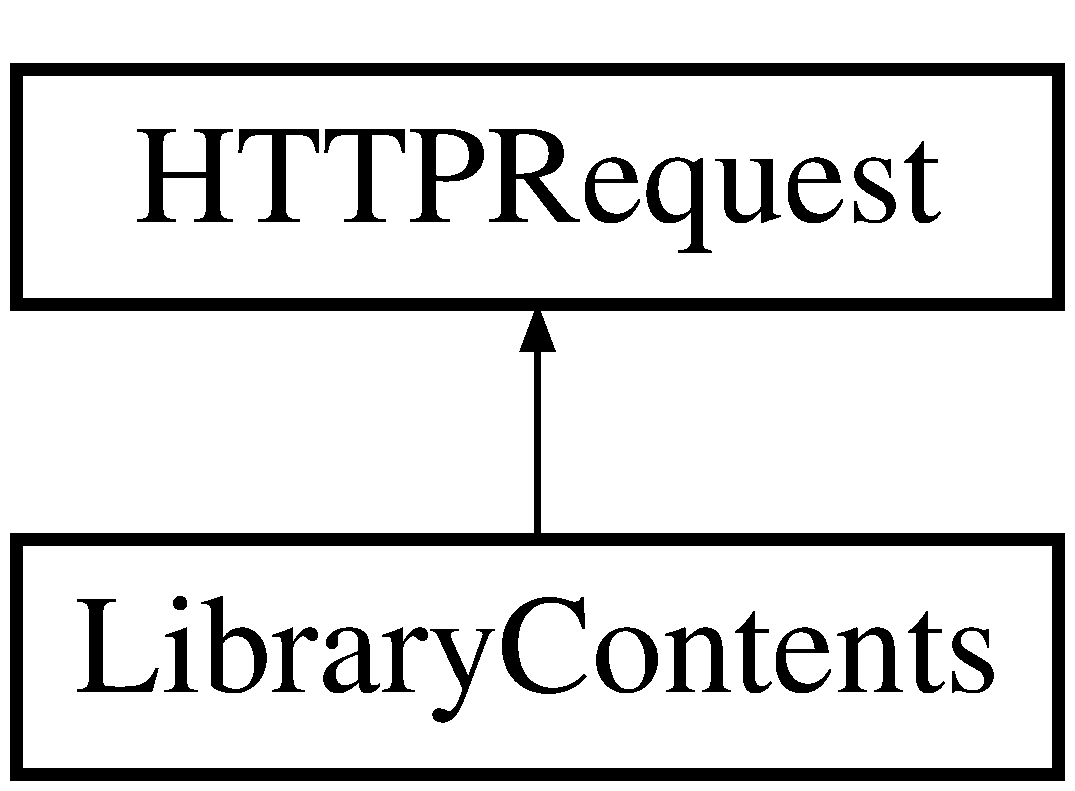
\includegraphics[height=2.000000cm]{classLibraryContents}
\end{center}
\end{figure}
\subsection*{Public Member Functions}
\begin{DoxyCompactItemize}
\item 
\hyperlink{classLibraryContents_a4426b4c31d1a6d79a4cf41c3c9de4622}{\+\_\+\+\_\+construct} (\$galaxy)
\item 
\hyperlink{classLibraryContents_a53a9170fe9857e34c33ac80e5daad546}{index} (\$library\+\_\+id)
\item 
\hyperlink{classLibraryContents_a6ef37835155eb3a1d6ca49245d12c21f}{show} (\$library\+\_\+id, \$library\+\_\+content\+\_\+id)
\item 
\hyperlink{classLibraryContents_ad6f818b7d72b436b40f47cab6f50b537}{create} (\$library\+\_\+id, \$folder\+\_\+id, \$create\+\_\+type, \$from\+\_\+hda\+\_\+id=N\+U\+LL, \$ldda\+\_\+message=N\+U\+LL, \$ldda\+\_\+message=N\+U\+LL, \$upload\+\_\+option=N\+U\+LL, \$server\+\_\+dir=N\+U\+LL, \$filesystem\+\_\+paths=N\+U\+LL, \$link\+\_\+data\+\_\+only=N\+U\+LL, \$name=N\+U\+LL, \$description=N\+U\+LL)
\end{DoxyCompactItemize}
\subsection*{Additional Inherited Members}


\subsection{Constructor \& Destructor Documentation}
\index{Library\+Contents@{Library\+Contents}!\+\_\+\+\_\+construct@{\+\_\+\+\_\+construct}}
\index{\+\_\+\+\_\+construct@{\+\_\+\+\_\+construct}!Library\+Contents@{Library\+Contents}}
\subsubsection[{\texorpdfstring{\+\_\+\+\_\+construct(\$galaxy)}{\_\_construct($galaxy)}}]{\setlength{\rightskip}{0pt plus 5cm}Library\+Contents\+::\+\_\+\+\_\+construct (
\begin{DoxyParamCaption}
\item[{}]{\$galaxy}
\end{DoxyParamCaption}
)}\hypertarget{classLibraryContents_a4426b4c31d1a6d79a4cf41c3c9de4622}{}\label{classLibraryContents_a4426b4c31d1a6d79a4cf41c3c9de4622}
The \hyperlink{classFolders}{Folders} constructor.


\begin{DoxyParams}[1]{Parameters}
\hyperlink{classGalaxyInstance}{Galaxy\+Instance} & {\em \$galaxy} & A \hyperlink{classGalaxyInstance}{Galaxy\+Instance} object.\\
\hline
\end{DoxyParams}
\begin{DoxyReturn}{Returns}
An instance of a \hyperlink{classLibraries}{Libraries} object. 
\end{DoxyReturn}


\subsection{Member Function Documentation}
\index{Library\+Contents@{Library\+Contents}!create@{create}}
\index{create@{create}!Library\+Contents@{Library\+Contents}}
\subsubsection[{\texorpdfstring{create(\$library\+\_\+id, \$folder\+\_\+id, \$create\+\_\+type, \$from\+\_\+hda\+\_\+id=\+N\+U\+L\+L, \$ldda\+\_\+message=\+N\+U\+L\+L, \$ldda\+\_\+message=\+N\+U\+L\+L, \$upload\+\_\+option=\+N\+U\+L\+L, \$server\+\_\+dir=\+N\+U\+L\+L, \$filesystem\+\_\+paths=\+N\+U\+L\+L, \$link\+\_\+data\+\_\+only=\+N\+U\+L\+L, \$name=\+N\+U\+L\+L, \$description=\+N\+U\+L\+L)}{create($library\_id, $folder\_id, $create\_type, $from\_hda\_id=NULL, $ldda\_message=NULL, $ldda\_message=NULL, $upload\_option=NULL, $server\_dir=NULL, $filesystem\_paths=NULL, $link\_data\_only=NULL, $name=NULL, $description=NULL)}}]{\setlength{\rightskip}{0pt plus 5cm}Library\+Contents\+::create (
\begin{DoxyParamCaption}
\item[{}]{\$library\+\_\+id, }
\item[{}]{\$folder\+\_\+id, }
\item[{}]{\$create\+\_\+type, }
\item[{}]{\$from\+\_\+hda\+\_\+id = {\ttfamily NULL}, }
\item[{}]{\$ldda\+\_\+message = {\ttfamily NULL}, }
\item[{}]{\$ldda\+\_\+message = {\ttfamily NULL}, }
\item[{}]{\$upload\+\_\+option = {\ttfamily NULL}, }
\item[{}]{\$server\+\_\+dir = {\ttfamily NULL}, }
\item[{}]{\$filesystem\+\_\+paths = {\ttfamily NULL}, }
\item[{}]{\$link\+\_\+data\+\_\+only = {\ttfamily NULL}, }
\item[{}]{\$name = {\ttfamily NULL}, }
\item[{}]{\$description = {\ttfamily NULL}}
\end{DoxyParamCaption}
)}\hypertarget{classLibraryContents_ad6f818b7d72b436b40f47cab6f50b537}{}\label{classLibraryContents_ad6f818b7d72b436b40f47cab6f50b537}
Add a folder/file/data collection to the specified the library.

This is one is important when you want to upload files to said library from a local filesystem to the given galaxy instance.


\begin{DoxyParams}{Parameters}
{\em \$library\+\_\+id} & \\
\hline
{\em \$folder\+\_\+id} & \\
\hline
{\em \$create\+\_\+type} & \\
\hline
{\em \$from\+\_\+hda\+\_\+id} & \\
\hline
{\em \$ldda\+\_\+message} & \\
\hline
{\em \$ldda\+\_\+message} & \\
\hline
{\em \$upload\+\_\+option} & \\
\hline
{\em \$server\+\_\+dir} & \\
\hline
{\em \$filesystem\+\_\+paths} & \\
\hline
{\em \$link\+\_\+data\+\_\+only} & \\
\hline
{\em \$name} & \\
\hline
{\em \$description} & \\
\hline
\end{DoxyParams}
\index{Library\+Contents@{Library\+Contents}!index@{index}}
\index{index@{index}!Library\+Contents@{Library\+Contents}}
\subsubsection[{\texorpdfstring{index(\$library\+\_\+id)}{index($library\_id)}}]{\setlength{\rightskip}{0pt plus 5cm}Library\+Contents\+::index (
\begin{DoxyParamCaption}
\item[{}]{\$library\+\_\+id}
\end{DoxyParamCaption}
)}\hypertarget{classLibraryContents_a53a9170fe9857e34c33ac80e5daad546}{}\label{classLibraryContents_a53a9170fe9857e34c33ac80e5daad546}
Gather the contents from the specified libarary.


\begin{DoxyParams}{Parameters}
{\em \$library\+\_\+id} & \\
\hline
\end{DoxyParams}
\begin{DoxyReturn}{Returns}
Files and \hyperlink{classFolders}{Folders} within the specified library. 
\end{DoxyReturn}
\index{Library\+Contents@{Library\+Contents}!show@{show}}
\index{show@{show}!Library\+Contents@{Library\+Contents}}
\subsubsection[{\texorpdfstring{show(\$library\+\_\+id, \$library\+\_\+content\+\_\+id)}{show($library\_id, $library\_content\_id)}}]{\setlength{\rightskip}{0pt plus 5cm}Library\+Contents\+::show (
\begin{DoxyParamCaption}
\item[{}]{\$library\+\_\+id, }
\item[{}]{\$library\+\_\+content\+\_\+id}
\end{DoxyParamCaption}
)}\hypertarget{classLibraryContents_a6ef37835155eb3a1d6ca49245d12c21f}{}\label{classLibraryContents_a6ef37835155eb3a1d6ca49245d12c21f}
View the specified library content within a given library.

You need both of the specific id\textquotesingle{}s in order to see the information of the content.


\begin{DoxyParams}{Parameters}
{\em \$library\+\_\+id} & \\
\hline
{\em \$library\+\_\+content\+\_\+id} & \\
\hline
\end{DoxyParams}
\begin{DoxyReturn}{Returns}
Detailed library item information. 
\end{DoxyReturn}


The documentation for this class was generated from the following file\+:\begin{DoxyCompactItemize}
\item 
Library\+Contents.\+inc\end{DoxyCompactItemize}

\hypertarget{classRequestError}{}\section{Request\+Error Class Reference}
\label{classRequestError}\index{Request\+Error@{Request\+Error}}
\subsection*{Public Member Functions}
\begin{DoxyCompactItemize}
\item 
\hyperlink{classRequestError_a06c774bf9df1e88166414494c0a0a2cf}{\+\_\+\+\_\+construct} ()
\item 
\hyperlink{classRequestError_a7b9cde1f37c70919c9370e1c1bae9570}{set\+Error} (\$type, \$message)
\item 
\hyperlink{classRequestError_a76a63d88399943e9cc34789f5b67ff24}{get\+Error} ()
\end{DoxyCompactItemize}


\subsection{Constructor \& Destructor Documentation}
\index{Request\+Error@{Request\+Error}!\+\_\+\+\_\+construct@{\+\_\+\+\_\+construct}}
\index{\+\_\+\+\_\+construct@{\+\_\+\+\_\+construct}!Request\+Error@{Request\+Error}}
\subsubsection[{\texorpdfstring{\+\_\+\+\_\+construct()}{\_\_construct()}}]{\setlength{\rightskip}{0pt plus 5cm}Request\+Error\+::\+\_\+\+\_\+construct (
\begin{DoxyParamCaption}
{}
\end{DoxyParamCaption}
)}\hypertarget{classRequestError_a06c774bf9df1e88166414494c0a0a2cf}{}\label{classRequestError_a06c774bf9df1e88166414494c0a0a2cf}
The Request Error constructor.

\begin{DoxyReturn}{Returns}
An instance of a Request Error object. 
\end{DoxyReturn}


\subsection{Member Function Documentation}
\index{Request\+Error@{Request\+Error}!get\+Error@{get\+Error}}
\index{get\+Error@{get\+Error}!Request\+Error@{Request\+Error}}
\subsubsection[{\texorpdfstring{get\+Error()}{getError()}}]{\setlength{\rightskip}{0pt plus 5cm}Request\+Error\+::get\+Error (
\begin{DoxyParamCaption}
{}
\end{DoxyParamCaption}
)}\hypertarget{classRequestError_a76a63d88399943e9cc34789f5b67ff24}{}\label{classRequestError_a76a63d88399943e9cc34789f5b67ff24}
Getter for this class\textquotesingle{}s \textquotesingle{}Error message\textquotesingle{} attribute.

\begin{DoxyReturn}{Returns}
The error message of the objet. 
\end{DoxyReturn}
\index{Request\+Error@{Request\+Error}!set\+Error@{set\+Error}}
\index{set\+Error@{set\+Error}!Request\+Error@{Request\+Error}}
\subsubsection[{\texorpdfstring{set\+Error(\$type, \$message)}{setError($type, $message)}}]{\setlength{\rightskip}{0pt plus 5cm}Request\+Error\+::set\+Error (
\begin{DoxyParamCaption}
\item[{}]{\$type, }
\item[{}]{\$message}
\end{DoxyParamCaption}
)}\hypertarget{classRequestError_a7b9cde1f37c70919c9370e1c1bae9570}{}\label{classRequestError_a7b9cde1f37c70919c9370e1c1bae9570}
Setter for the class\textquotesingle{}s \textquotesingle{}Error\textquotesingle{} attribute


\begin{DoxyParams}{Parameters}
{\em \$type} & Type of Error. Typical types are \textquotesingle{}H\+T\+TP\textquotesingle{} or \textquotesingle{}Galaxy\textquotesingle{}. \\
\hline
{\em \$message} & The Error message. \\
\hline
\end{DoxyParams}


The documentation for this class was generated from the following file\+:\begin{DoxyCompactItemize}
\item 
\hyperlink{RequestError_8inc}{Request\+Error.\+inc}\end{DoxyCompactItemize}

\hypertarget{classRequests}{}\section{Requests Class Reference}
\label{classRequests}\index{Requests@{Requests}}
Inheritance diagram for Requests\+:\begin{figure}[H]
\begin{center}
\leavevmode
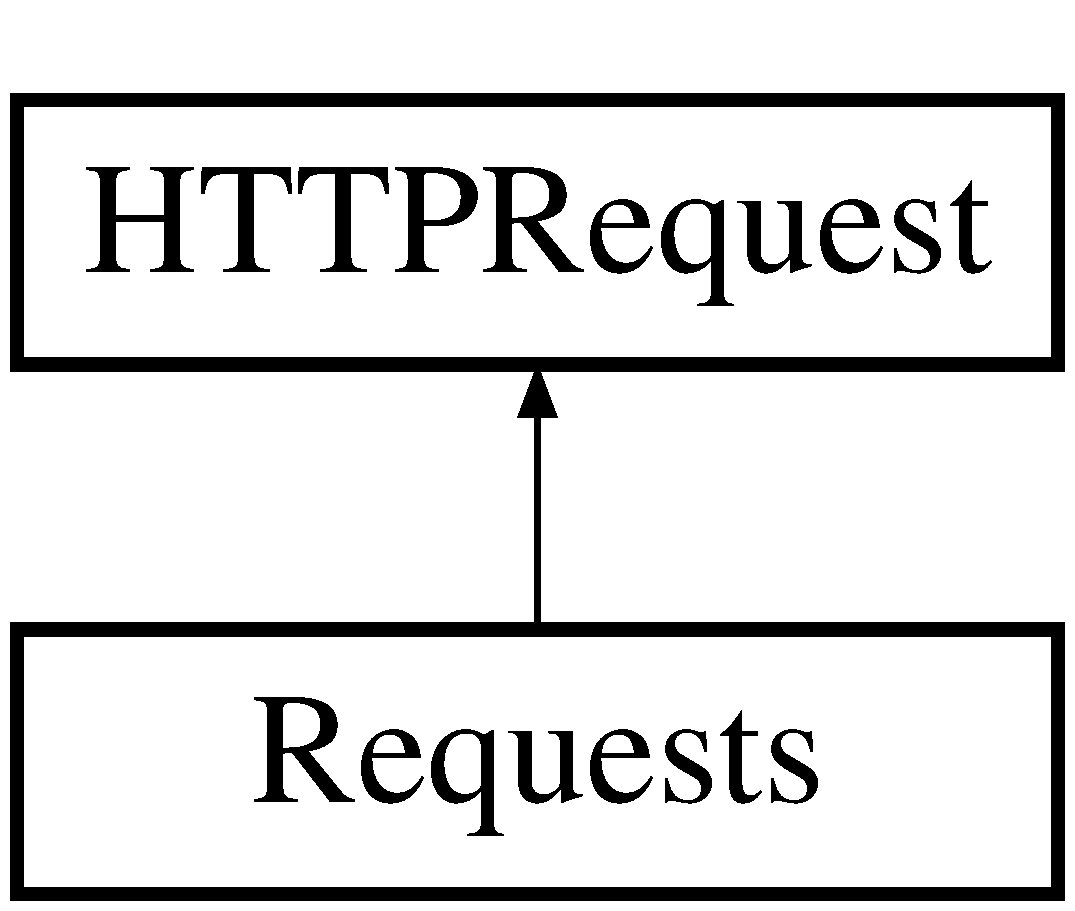
\includegraphics[height=2.000000cm]{classRequests}
\end{center}
\end{figure}
\subsection*{Public Member Functions}
\begin{DoxyCompactItemize}
\item 
\hyperlink{classRequests_ad4f6b224dace74a82e24345455de19e7}{\+\_\+\+\_\+construct} (\$galaxy)
\item 
\hyperlink{classRequests_ae974e9e6c8ac78bea994e66ee3f1c65f}{index} ()
\item 
\hyperlink{classRequests_a767527fe7a23f41746ad123af5a4271d}{show} (\$encoded\+\_\+request\+\_\+id)
\item 
\hyperlink{classRequests_a493a6e9e3597e39070464a9424f2d6ff}{update} (\$encoded\+\_\+request\+\_\+id)
\end{DoxyCompactItemize}
\subsection*{Additional Inherited Members}


\subsection{Constructor \& Destructor Documentation}
\index{Requests@{Requests}!\+\_\+\+\_\+construct@{\+\_\+\+\_\+construct}}
\index{\+\_\+\+\_\+construct@{\+\_\+\+\_\+construct}!Requests@{Requests}}
\subsubsection[{\texorpdfstring{\+\_\+\+\_\+construct(\$galaxy)}{\_\_construct($galaxy)}}]{\setlength{\rightskip}{0pt plus 5cm}Requests\+::\+\_\+\+\_\+construct (
\begin{DoxyParamCaption}
\item[{}]{\$galaxy}
\end{DoxyParamCaption}
)}\hypertarget{classRequests_ad4f6b224dace74a82e24345455de19e7}{}\label{classRequests_ad4f6b224dace74a82e24345455de19e7}
The Request constructor.

\begin{DoxyReturn}{Returns}
An instance of a Request object. 
\end{DoxyReturn}


\subsection{Member Function Documentation}
\index{Requests@{Requests}!index@{index}}
\index{index@{index}!Requests@{Requests}}
\subsubsection[{\texorpdfstring{index()}{index()}}]{\setlength{\rightskip}{0pt plus 5cm}Requests\+::index (
\begin{DoxyParamCaption}
{}
\end{DoxyParamCaption}
)}\hypertarget{classRequests_ae974e9e6c8ac78bea994e66ee3f1c65f}{}\label{classRequests_ae974e9e6c8ac78bea994e66ee3f1c65f}
Displays a collection (list) of sequencing requests.

\begin{DoxyReturn}{Returns}
An array of the requests. 
\end{DoxyReturn}
\index{Requests@{Requests}!show@{show}}
\index{show@{show}!Requests@{Requests}}
\subsubsection[{\texorpdfstring{show(\$encoded\+\_\+request\+\_\+id)}{show($encoded\_request\_id)}}]{\setlength{\rightskip}{0pt plus 5cm}Requests\+::show (
\begin{DoxyParamCaption}
\item[{}]{\$encoded\+\_\+request\+\_\+id}
\end{DoxyParamCaption}
)}\hypertarget{classRequests_a767527fe7a23f41746ad123af5a4271d}{}\label{classRequests_a767527fe7a23f41746ad123af5a4271d}
Displays details of a sequencing request.

G\+ET /api/requests/\{encoded\+\_\+request\+\_\+id\}


\begin{DoxyParams}{Parameters}
{\em encoded\+\_\+request\+\_\+id} & The id of the galaxy entity to show.\\
\hline
\end{DoxyParams}
\begin{DoxyReturn}{Returns}
An array containing detailed information about the requested galaxy entitiy. 
\end{DoxyReturn}
\index{Requests@{Requests}!update@{update}}
\index{update@{update}!Requests@{Requests}}
\subsubsection[{\texorpdfstring{update(\$encoded\+\_\+request\+\_\+id)}{update($encoded\_request\_id)}}]{\setlength{\rightskip}{0pt plus 5cm}Requests\+::update (
\begin{DoxyParamCaption}
\item[{}]{\$encoded\+\_\+request\+\_\+id}
\end{DoxyParamCaption}
)}\hypertarget{classRequests_a493a6e9e3597e39070464a9424f2d6ff}{}\label{classRequests_a493a6e9e3597e39070464a9424f2d6ff}
Updates a request state, sample state or sample dataset transfer status.


\begin{DoxyParams}{Parameters}
{\em \$encoded\+\_\+request\+\_\+id} & The id of the galaxy entity to update.\\
\hline
\end{DoxyParams}
\begin{DoxyReturn}{Returns}
An array containing information on the updated Galaxy entity. 
\end{DoxyReturn}


The documentation for this class was generated from the following file\+:\begin{DoxyCompactItemize}
\item 
\hyperlink{Requests_8inc}{Requests.\+inc}\end{DoxyCompactItemize}

\hypertarget{classRoles}{}\section{Roles Class Reference}
\label{classRoles}\index{Roles@{Roles}}
Inheritance diagram for Roles\+:\begin{figure}[H]
\begin{center}
\leavevmode
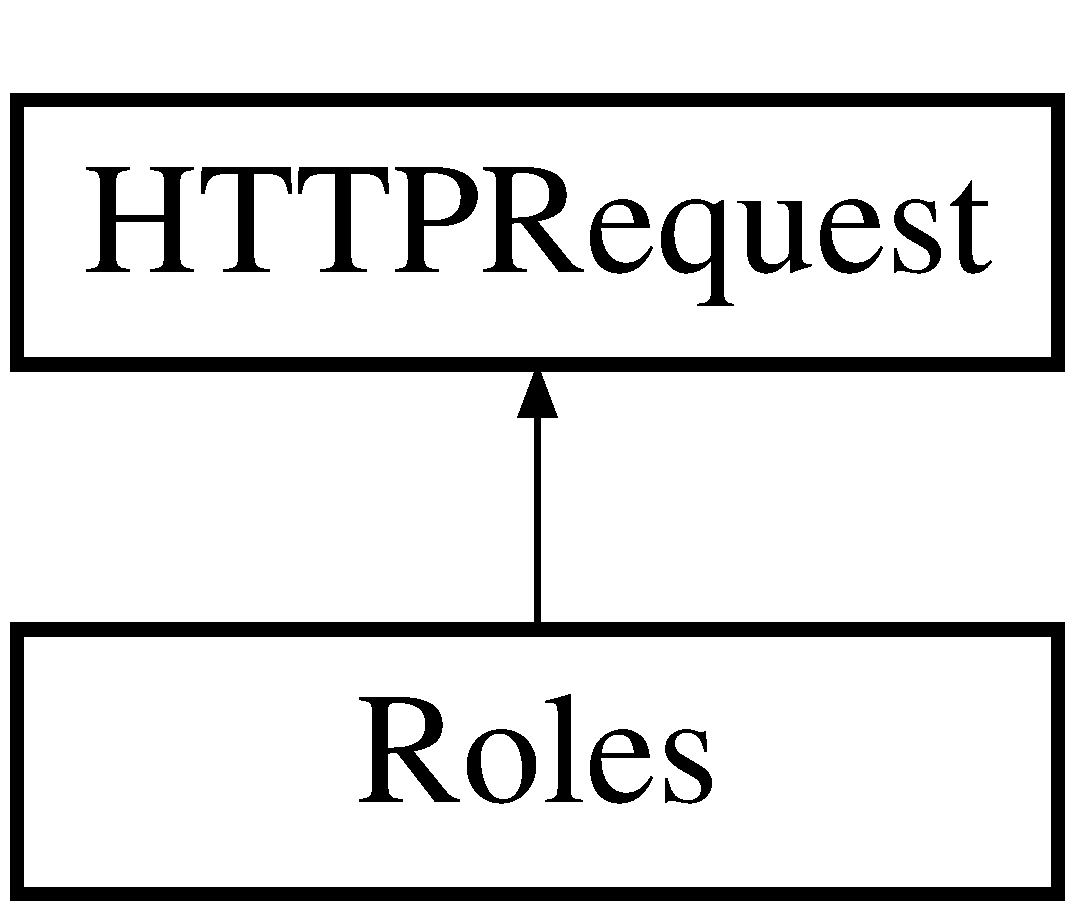
\includegraphics[height=2.000000cm]{classRoles}
\end{center}
\end{figure}
\subsection*{Public Member Functions}
\begin{DoxyCompactItemize}
\item 
\hyperlink{classRoles_a04f770a838907223185f262942c1ed61}{\+\_\+\+\_\+construct} (\$galaxy)
\item 
\hyperlink{classRoles_a176d68692a0e165d82e95026e27ad85e}{index} ()
\item 
\hyperlink{classRoles_ae6e8905552f27d885368d5f2dae00f8d}{show} (\$role\+\_\+id)
\item 
\hyperlink{classRoles_ae7b1294d10eb7488dfb28bd98bd9823c}{create} (\$name, \$description, \$user\+\_\+ids=array(), \$group\+\_\+ids=array())
\end{DoxyCompactItemize}
\subsection*{Additional Inherited Members}


\subsection{Constructor \& Destructor Documentation}
\index{Roles@{Roles}!\+\_\+\+\_\+construct@{\+\_\+\+\_\+construct}}
\index{\+\_\+\+\_\+construct@{\+\_\+\+\_\+construct}!Roles@{Roles}}
\subsubsection[{\texorpdfstring{\+\_\+\+\_\+construct(\$galaxy)}{\_\_construct($galaxy)}}]{\setlength{\rightskip}{0pt plus 5cm}Roles\+::\+\_\+\+\_\+construct (
\begin{DoxyParamCaption}
\item[{}]{\$galaxy}
\end{DoxyParamCaption}
)}\hypertarget{classRoles_a04f770a838907223185f262942c1ed61}{}\label{classRoles_a04f770a838907223185f262942c1ed61}
The \hyperlink{classRoles}{Roles} constructor.


\begin{DoxyParams}[1]{Parameters}
\hyperlink{classGalaxyInstance}{Galaxy\+Instance} & {\em \$galaxy} & A \hyperlink{classGalaxyInstance}{Galaxy\+Instance} object.\\
\hline
\end{DoxyParams}
\begin{DoxyReturn}{Returns}
An instance of a roles object. 
\end{DoxyReturn}


\subsection{Member Function Documentation}
\index{Roles@{Roles}!create@{create}}
\index{create@{create}!Roles@{Roles}}
\subsubsection[{\texorpdfstring{create(\$name, \$description, \$user\+\_\+ids=array(), \$group\+\_\+ids=array())}{create($name, $description, $user\_ids=array(), $group\_ids=array())}}]{\setlength{\rightskip}{0pt plus 5cm}Roles\+::create (
\begin{DoxyParamCaption}
\item[{}]{\$name, }
\item[{}]{\$description, }
\item[{}]{\$user\+\_\+ids = {\ttfamily array()}, }
\item[{}]{\$group\+\_\+ids = {\ttfamily array()}}
\end{DoxyParamCaption}
)}\hypertarget{classRoles_ae7b1294d10eb7488dfb28bd98bd9823c}{}\label{classRoles_ae7b1294d10eb7488dfb28bd98bd9823c}
Creates a new role.

Corresponds to the Galaxy Api/path\+: P\+O\+ST /api/roles N\+O\+TE\+: only type admin can be applied for new roles


\begin{DoxyParams}{Parameters}
{\em \$name} & The name of the new role. \\
\hline
{\em \$description} & The description of the new role. \\
\hline
{\em \$user\+\_\+ids} & An array of user ids to associate the new role with. To obtain a user id, please use the \hyperlink{classRoles_a176d68692a0e165d82e95026e27ad85e}{index()} function of the users class. \\
\hline
{\em \$group\+\_\+ids} & An array of group id\textquotesingle{}s to associate the new role with. To obtain a group id, please use the \hyperlink{classRoles_a176d68692a0e165d82e95026e27ad85e}{index()} function of the groups class.\\
\hline
\end{DoxyParams}
\begin{DoxyReturn}{Returns}
An array containing informaiton about the new role. 
\end{DoxyReturn}
\index{Roles@{Roles}!index@{index}}
\index{index@{index}!Roles@{Roles}}
\subsubsection[{\texorpdfstring{index()}{index()}}]{\setlength{\rightskip}{0pt plus 5cm}Roles\+::index (
\begin{DoxyParamCaption}
{}
\end{DoxyParamCaption}
)}\hypertarget{classRoles_a176d68692a0e165d82e95026e27ad85e}{}\label{classRoles_a176d68692a0e165d82e95026e27ad85e}
Retreive a list of all of Galaxy\textquotesingle{}s roles.

Corresponds to the Galaxy A\+P\+I/path\+: G\+ET /api/roles

\begin{DoxyReturn}{Returns}
An array containing details of all the roles in Galaxy. 
\end{DoxyReturn}
\index{Roles@{Roles}!show@{show}}
\index{show@{show}!Roles@{Roles}}
\subsubsection[{\texorpdfstring{show(\$role\+\_\+id)}{show($role\_id)}}]{\setlength{\rightskip}{0pt plus 5cm}Roles\+::show (
\begin{DoxyParamCaption}
\item[{}]{\$role\+\_\+id}
\end{DoxyParamCaption}
)}\hypertarget{classRoles_ae6e8905552f27d885368d5f2dae00f8d}{}\label{classRoles_ae6e8905552f27d885368d5f2dae00f8d}
Retreive details about a specific Galaxy role.

Corresponds to the Galaxy A\+P\+I/path\+: G\+ET /api/roles/\{encoded\+\_\+id\}


\begin{DoxyParams}{Parameters}
{\em \$role\+\_\+id} & The id of the role whos informaiton to retreive. Please use this class\textquotesingle{}s index function to retreive a list of role id\textquotesingle{}s.\\
\hline
\end{DoxyParams}
\begin{DoxyReturn}{Returns}
An array containing details about the specified role. 
\end{DoxyReturn}


The documentation for this class was generated from the following file\+:\begin{DoxyCompactItemize}
\item 
\hyperlink{Roles_8inc}{Roles.\+inc}\end{DoxyCompactItemize}

\hypertarget{classSearch}{}\section{Search Class Reference}
\label{classSearch}\index{Search@{Search}}
Inheritance diagram for Search\+:\begin{figure}[H]
\begin{center}
\leavevmode
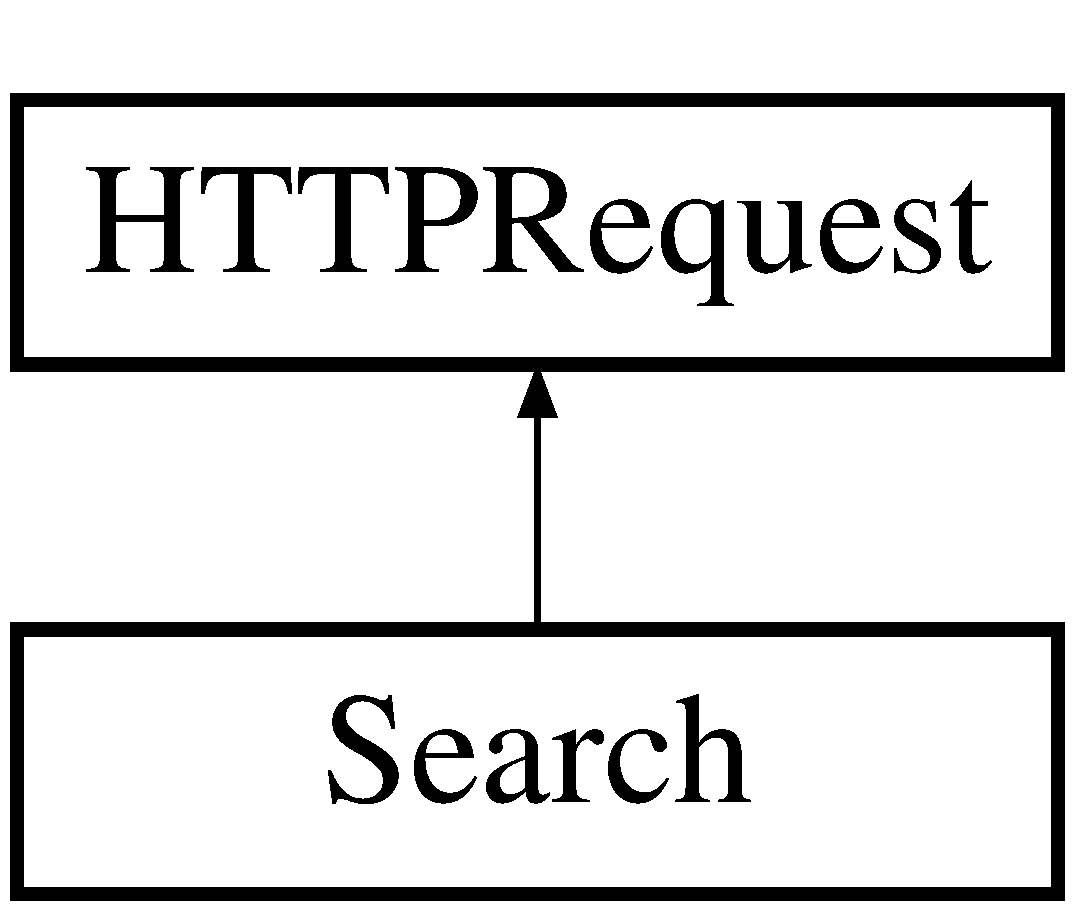
\includegraphics[height=2.000000cm]{classSearch}
\end{center}
\end{figure}
\subsection*{Public Member Functions}
\begin{DoxyCompactItemize}
\item 
\hyperlink{classSearch_a2800566c87716cf24ec86604e1a23495}{\+\_\+\+\_\+construct} (\$galaxy)
\item 
\hyperlink{classSearch_af1cd89ca839300909cfebf24e76c9434}{create} (\$query)
\end{DoxyCompactItemize}
\subsection*{Additional Inherited Members}


\subsection{Constructor \& Destructor Documentation}
\index{Search@{Search}!\+\_\+\+\_\+construct@{\+\_\+\+\_\+construct}}
\index{\+\_\+\+\_\+construct@{\+\_\+\+\_\+construct}!Search@{Search}}
\subsubsection[{\texorpdfstring{\+\_\+\+\_\+construct(\$galaxy)}{\_\_construct($galaxy)}}]{\setlength{\rightskip}{0pt plus 5cm}Search\+::\+\_\+\+\_\+construct (
\begin{DoxyParamCaption}
\item[{}]{\$galaxy}
\end{DoxyParamCaption}
)}\hypertarget{classSearch_a2800566c87716cf24ec86604e1a23495}{}\label{classSearch_a2800566c87716cf24ec86604e1a23495}
Implements the \hyperlink{classSearch}{Search} constructor.


\begin{DoxyParams}{Parameters}
{\em \hyperlink{classGalaxyInstance}{Galaxy\+Instance}} & galaxy A Galaxy Instance object.\\
\hline
\end{DoxyParams}
\begin{DoxyReturn}{Returns}
An instance of a search object. 
\end{DoxyReturn}


\subsection{Member Function Documentation}
\index{Search@{Search}!create@{create}}
\index{create@{create}!Search@{Search}}
\subsubsection[{\texorpdfstring{create(\$query)}{create($query)}}]{\setlength{\rightskip}{0pt plus 5cm}Search\+::create (
\begin{DoxyParamCaption}
\item[{}]{\$query}
\end{DoxyParamCaption}
)}\hypertarget{classSearch_af1cd89ca839300909cfebf24e76c9434}{}\label{classSearch_af1cd89ca839300909cfebf24e76c9434}
Performs a search of the various elements in Galaxy.

Corresponds to the galaxy method/path\+: Post /api/search


\begin{DoxyParams}{Parameters}
{\em \$query,must} & be a valid, lowercase, S\+QL expression, example\+: \textquotesingle{}select $\ast$ from history where id = \textbackslash{}\textquotesingle{}290670ee50ab85f0\textbackslash{}\textquotesingle{}\textquotesingle{}\\
\hline
\end{DoxyParams}
\begin{DoxyReturn}{Returns}
An array of the Galaxy elements that matches the query. 
\end{DoxyReturn}


The documentation for this class was generated from the following file\+:\begin{DoxyCompactItemize}
\item 
\hyperlink{Search_8inc}{Search.\+inc}\end{DoxyCompactItemize}

\hypertarget{classTools}{}\section{Tools Class Reference}
\label{classTools}\index{Tools@{Tools}}
Inheritance diagram for Tools\+:\begin{figure}[H]
\begin{center}
\leavevmode
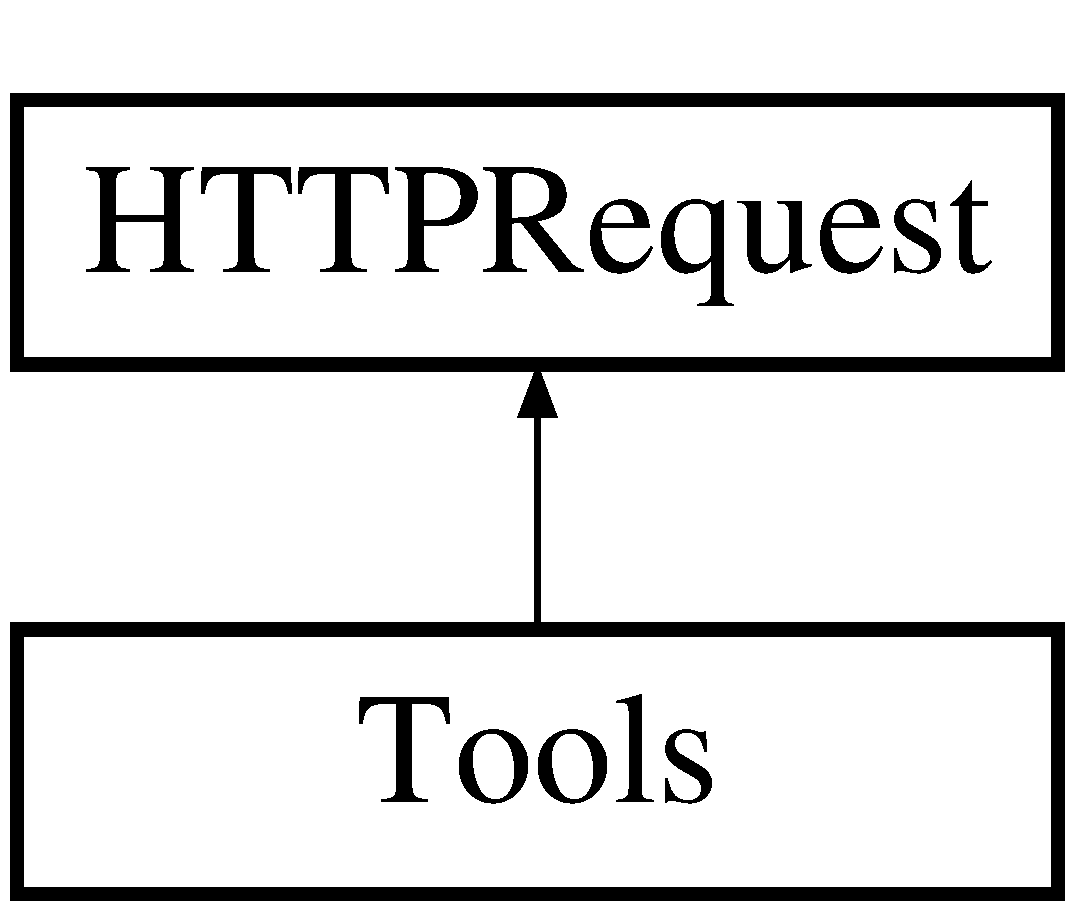
\includegraphics[height=2.000000cm]{classTools}
\end{center}
\end{figure}
\subsection*{Public Member Functions}
\begin{DoxyCompactItemize}
\item 
\hyperlink{classTools_a6c92297b66e27e21e3b68e037870b61b}{\+\_\+\+\_\+construct} (\$galaxy)
\item 
\hyperlink{classTools_a1875c4619e668075faccf1a2f0cdd118}{index} (\$tool\+\_\+id=N\+U\+LL, \$q=N\+U\+LL, \$in\+\_\+panel=F\+A\+L\+SE, \$trackster=F\+A\+L\+SE)
\item 
\hyperlink{classTools_a4a86784cc0d4a366ba12e5ee736b6c0b}{show} (\$tool\+\_\+id)
\item 
\hyperlink{classTools_a6399f14dc2742734aac118c71896e77e}{diagnostics} (\$tool\+\_\+id)
\item 
\hyperlink{classTools_af681de7d892bf2b17d388d63534a45f9}{reload} (\$tool\+\_\+id)
\item 
\hyperlink{classTools_aa367ad2e9641a3e7cba7a48a1927de89}{build} (\$tool\+\_\+id, \$history\+\_\+id, \$tool\+\_\+version=N\+U\+LL)
\item 
\hyperlink{classTools_adf67dfe22f68133f3a7a68950b9f3ec9}{citations} (\$tool\+\_\+id)
\item 
\hyperlink{classTools_a355eb988d4bbd7f3b28b505e4c950d58}{download} (\$tool\+\_\+id, \$file\+\_\+path)
\item 
\hyperlink{classTools_a94a6d817eda85b60d90943049e50808f}{create} (\$tool\+\_\+id, \$history\+\_\+id, \$files=N\+U\+LL, \$input\+\_\+dataset\+\_\+ids=array(), \$tool\+\_\+version=N\+U\+LL, \$region=N\+U\+LL, \$action=N\+U\+LL)
\end{DoxyCompactItemize}
\subsection*{Additional Inherited Members}


\subsection{Constructor \& Destructor Documentation}
\index{Tools@{Tools}!\+\_\+\+\_\+construct@{\+\_\+\+\_\+construct}}
\index{\+\_\+\+\_\+construct@{\+\_\+\+\_\+construct}!Tools@{Tools}}
\subsubsection[{\texorpdfstring{\+\_\+\+\_\+construct(\$galaxy)}{\_\_construct($galaxy)}}]{\setlength{\rightskip}{0pt plus 5cm}Tools\+::\+\_\+\+\_\+construct (
\begin{DoxyParamCaption}
\item[{}]{\$galaxy}
\end{DoxyParamCaption}
)}\hypertarget{classTools_a6c92297b66e27e21e3b68e037870b61b}{}\label{classTools_a6c92297b66e27e21e3b68e037870b61b}
The \hyperlink{classTools}{Tools} constructor.


\begin{DoxyParams}[1]{Parameters}
\hyperlink{classGalaxyInstance}{Galaxy\+Instance} & {\em \$galaxy} & A \hyperlink{classGalaxyInstance}{Galaxy\+Instance} object.\\
\hline
\end{DoxyParams}
\begin{DoxyReturn}{Returns}
An instance of a \hyperlink{classTools}{Tools} object. 
\end{DoxyReturn}


\subsection{Member Function Documentation}
\index{Tools@{Tools}!build@{build}}
\index{build@{build}!Tools@{Tools}}
\subsubsection[{\texorpdfstring{build(\$tool\+\_\+id, \$history\+\_\+id, \$tool\+\_\+version=\+N\+U\+L\+L)}{build($tool\_id, $history\_id, $tool\_version=NULL)}}]{\setlength{\rightskip}{0pt plus 5cm}Tools\+::build (
\begin{DoxyParamCaption}
\item[{}]{\$tool\+\_\+id, }
\item[{}]{\$history\+\_\+id, }
\item[{}]{\$tool\+\_\+version = {\ttfamily NULL}}
\end{DoxyParamCaption}
)}\hypertarget{classTools_aa367ad2e9641a3e7cba7a48a1927de89}{}\label{classTools_aa367ad2e9641a3e7cba7a48a1927de89}
Returns a tool model that includes its parameters.

Corresponds to the Galaxy A\+P\+I/path G\+ET /api/tools/\{tool\+\_\+id\}/build

Note the original python function allows for an \textquotesingle{}inputs\textquotesingle{} parameter, this is not supported here.


\begin{DoxyParams}{Parameters}
{\em \$tool\+\_\+id} & id of the tool to perform this aciton on. Please use this class\textquotesingle{}s \hyperlink{classTools_a1875c4619e668075faccf1a2f0cdd118}{index()} function to retreive a tool id. \\
\hline
{\em history\+\_\+id} & The id of the history to place the built tool. \\
\hline
{\em \$tool\+\_\+version} & Optional, the version of the tool.\\
\hline
\end{DoxyParams}
\begin{DoxyReturn}{Returns}
An array containing the build model of the tool. 
\end{DoxyReturn}
\index{Tools@{Tools}!citations@{citations}}
\index{citations@{citations}!Tools@{Tools}}
\subsubsection[{\texorpdfstring{citations(\$tool\+\_\+id)}{citations($tool\_id)}}]{\setlength{\rightskip}{0pt plus 5cm}Tools\+::citations (
\begin{DoxyParamCaption}
\item[{}]{\$tool\+\_\+id}
\end{DoxyParamCaption}
)}\hypertarget{classTools_adf67dfe22f68133f3a7a68950b9f3ec9}{}\label{classTools_adf67dfe22f68133f3a7a68950b9f3ec9}
Retreive the citations for a given tool.

Corresponds to the Galaxy Api/path G\+ET /api/tools/\{tool\+\_\+id\}/citations


\begin{DoxyParams}{Parameters}
{\em \$tool\+\_\+id} & The id of the specified tool. To obtain a tool id, please use this class\textquotesingle{} \hyperlink{classTools_a1875c4619e668075faccf1a2f0cdd118}{index()} function.\\
\hline
\end{DoxyParams}
\begin{DoxyReturn}{Returns}
An array containing infromation about the citations of the specified tool. 
\end{DoxyReturn}
\index{Tools@{Tools}!create@{create}}
\index{create@{create}!Tools@{Tools}}
\subsubsection[{\texorpdfstring{create(\$tool\+\_\+id, \$history\+\_\+id, \$files=\+N\+U\+L\+L, \$input\+\_\+dataset\+\_\+ids=array(), \$tool\+\_\+version=\+N\+U\+L\+L, \$region=\+N\+U\+L\+L, \$action=\+N\+U\+L\+L)}{create($tool\_id, $history\_id, $files=NULL, $input\_dataset\_ids=array(), $tool\_version=NULL, $region=NULL, $action=NULL)}}]{\setlength{\rightskip}{0pt plus 5cm}Tools\+::create (
\begin{DoxyParamCaption}
\item[{}]{\$tool\+\_\+id, }
\item[{}]{\$history\+\_\+id, }
\item[{}]{\$files = {\ttfamily NULL}, }
\item[{}]{\$input\+\_\+dataset\+\_\+ids = {\ttfamily array()}, }
\item[{}]{\$tool\+\_\+version = {\ttfamily NULL}, }
\item[{}]{\$region = {\ttfamily NULL}, }
\item[{}]{\$action = {\ttfamily NULL}}
\end{DoxyParamCaption}
)}\hypertarget{classTools_a94a6d817eda85b60d90943049e50808f}{}\label{classTools_a94a6d817eda85b60d90943049e50808f}
Executes a tool using specified inputs.

Corresponds to the Galaxy A\+P\+I/path at P\+O\+ST /api/tools


\begin{DoxyParams}{Parameters}
{\em \$tool\+\_\+id} & The id of the specified tool. To obtain a tool id, please use this class \hyperlink{classTools_a1875c4619e668075faccf1a2f0cdd118}{index()} function. \\
\hline
{\em history\+\_\+id} & The history\+\_\+id where the tool is located. To obtain history id\textquotesingle{}s please see the history class. \\
\hline
{\em files} & an array of file infromation, the array should be N\+U\+LL or in the following format\+: \$files = array( 0 =$>$ array( \textquotesingle{}name\textquotesingle{} =$>$ \mbox{[}file name\mbox{]}, \textquotesingle{}path\textquotesingle{} =$>$ \mbox{[}full path to the file\mbox{]}, ), 1 =$>$ array( \textquotesingle{}name\textquotesingle{} =$>$ \mbox{[}file name\mbox{]}, \textquotesingle{}path\textquotesingle{} =$>$ \mbox{[}full path to the file\mbox{]}, ), ... ); where index i of filepaths and index i of filenames corresponds to the same file. \\
\hline
{\em input\+\_\+dataset\+\_\+ds} & Array of dataset id\textquotesingle{}s where the tool should grab the inputs from. Please see the datasets class to obtain id\textquotesingle{}s. \\
\hline
{\em tool\+\_\+version} & Optional, specify specific tool version for the tool. \\
\hline
{\em region} & Optional information on the region of the genome being rerun. \\
\hline
{\em action} & Optional, \textquotesingle{}rerun\textquotesingle{} to rerun the tool and not execute\\
\hline
\end{DoxyParams}
\begin{DoxyReturn}{Returns}
An array containing information about the created or executed tool. 
\end{DoxyReturn}
\index{Tools@{Tools}!diagnostics@{diagnostics}}
\index{diagnostics@{diagnostics}!Tools@{Tools}}
\subsubsection[{\texorpdfstring{diagnostics(\$tool\+\_\+id)}{diagnostics($tool\_id)}}]{\setlength{\rightskip}{0pt plus 5cm}Tools\+::diagnostics (
\begin{DoxyParamCaption}
\item[{}]{\$tool\+\_\+id}
\end{DoxyParamCaption}
)}\hypertarget{classTools_a6399f14dc2742734aac118c71896e77e}{}\label{classTools_a6399f14dc2742734aac118c71896e77e}
Return diagnostic information about a tool.

Corresponds to the Galaxy A\+P\+I/path at G\+ET /api/tools/\{tool\+\_\+id\}/diagnostics


\begin{DoxyParams}{Parameters}
{\em \$tool\+\_\+id} & The id of the tool to retreive diagnostics from, to obtain a tool id please see this class\textquotesingle{}s index function.\\
\hline
\end{DoxyParams}
\begin{DoxyReturn}{Returns}
An array contaiing information about the diagnostics of a tool. 
\end{DoxyReturn}
\index{Tools@{Tools}!download@{download}}
\index{download@{download}!Tools@{Tools}}
\subsubsection[{\texorpdfstring{download(\$tool\+\_\+id, \$file\+\_\+path)}{download($tool\_id, $file\_path)}}]{\setlength{\rightskip}{0pt plus 5cm}Tools\+::download (
\begin{DoxyParamCaption}
\item[{}]{\$tool\+\_\+id, }
\item[{}]{\$file\+\_\+path}
\end{DoxyParamCaption}
)}\hypertarget{classTools_a355eb988d4bbd7f3b28b505e4c950d58}{}\label{classTools_a355eb988d4bbd7f3b28b505e4c950d58}
Download a specified tool.

Corresponds to the Galaxy Api/\+Path at\+: G\+ET /api/tools/\{tool\+\_\+id\}/download


\begin{DoxyParams}{Parameters}
{\em \$tool\+\_\+id} & The id of the specified tool. To obtain a tool id, please use this class \hyperlink{classTools_a1875c4619e668075faccf1a2f0cdd118}{index()} function.\\
\hline
{\em \$file\+\_\+path} & The path to where the file will be stored.\\
\hline
\end{DoxyParams}
\begin{DoxyReturn}{Returns}
Gzip of the tool. 
\end{DoxyReturn}
\index{Tools@{Tools}!index@{index}}
\index{index@{index}!Tools@{Tools}}
\subsubsection[{\texorpdfstring{index(\$tool\+\_\+id=\+N\+U\+L\+L, \$q=\+N\+U\+L\+L, \$in\+\_\+panel=\+F\+A\+L\+S\+E, \$trackster=\+F\+A\+L\+S\+E)}{index($tool\_id=NULL, $q=NULL, $in\_panel=FALSE, $trackster=FALSE)}}]{\setlength{\rightskip}{0pt plus 5cm}Tools\+::index (
\begin{DoxyParamCaption}
\item[{}]{\$tool\+\_\+id = {\ttfamily NULL}, }
\item[{}]{\$q = {\ttfamily NULL}, }
\item[{}]{\$in\+\_\+panel = {\ttfamily FALSE}, }
\item[{}]{\$trackster = {\ttfamily FALSE}}
\end{DoxyParamCaption}
)}\hypertarget{classTools_a1875c4619e668075faccf1a2f0cdd118}{}\label{classTools_a1875c4619e668075faccf1a2f0cdd118}
Retreive a list of tools defined by the parameters.

Corresponds to the Galaxy A\+P\+I/path\+: G\+ET /api/tools\+:


\begin{DoxyParams}{Parameters}
{\em \$tool\+\_\+id} & Optional, the id of the tool to specify. \\
\hline
{\em \$q} & Optional, additional search details. \\
\hline
{\em \$in\+\_\+panel} & If true, return tools marked as in panel. \\
\hline
{\em \$trackster} & If true, return tools marked as trackster.\\
\hline
\end{DoxyParams}
\begin{DoxyReturn}{Returns}
An array containing all the tools in galaxy that match the the specified search. 
\end{DoxyReturn}
\index{Tools@{Tools}!reload@{reload}}
\index{reload@{reload}!Tools@{Tools}}
\subsubsection[{\texorpdfstring{reload(\$tool\+\_\+id)}{reload($tool\_id)}}]{\setlength{\rightskip}{0pt plus 5cm}Tools\+::reload (
\begin{DoxyParamCaption}
\item[{}]{\$tool\+\_\+id}
\end{DoxyParamCaption}
)}\hypertarget{classTools_af681de7d892bf2b17d388d63534a45f9}{}\label{classTools_af681de7d892bf2b17d388d63534a45f9}
Reload specified tool.

Corresponds to the Galaxy Api/path G\+ET /api/tools/\{tool\+\_\+id\}/reload


\begin{DoxyParams}{Parameters}
{\em \$tool\+\_\+id} & The id of the tool to reload.\\
\hline
\end{DoxyParams}
\begin{DoxyReturn}{Returns}
An array of the tool that was reloaded. 
\end{DoxyReturn}
\index{Tools@{Tools}!show@{show}}
\index{show@{show}!Tools@{Tools}}
\subsubsection[{\texorpdfstring{show(\$tool\+\_\+id)}{show($tool\_id)}}]{\setlength{\rightskip}{0pt plus 5cm}Tools\+::show (
\begin{DoxyParamCaption}
\item[{}]{\$tool\+\_\+id}
\end{DoxyParamCaption}
)}\hypertarget{classTools_a4a86784cc0d4a366ba12e5ee736b6c0b}{}\label{classTools_a4a86784cc0d4a366ba12e5ee736b6c0b}
Retreives detailed informaiton of a specific tool.

Corresponds to the Galaxy A\+P\+I/path G\+ET /api/tools/\{tool\+\_\+id\}


\begin{DoxyParams}{Parameters}
{\em \$tool\+\_\+id} & The id of the tool whos informaiton to obtain. To retreive a tool id please use this class\textquotesingle{}s index funciton.\\
\hline
\end{DoxyParams}
\begin{DoxyReturn}{Returns}
An array containing detailed information about a specific tool. 
\end{DoxyReturn}


The documentation for this class was generated from the following file\+:\begin{DoxyCompactItemize}
\item 
\hyperlink{Tools_8inc}{Tools.\+inc}\end{DoxyCompactItemize}

\hypertarget{classToolShedRepositories}{}\section{Tool\+Shed\+Repositories Class Reference}
\label{classToolShedRepositories}\index{Tool\+Shed\+Repositories@{Tool\+Shed\+Repositories}}
Inheritance diagram for Tool\+Shed\+Repositories\+:\begin{figure}[H]
\begin{center}
\leavevmode
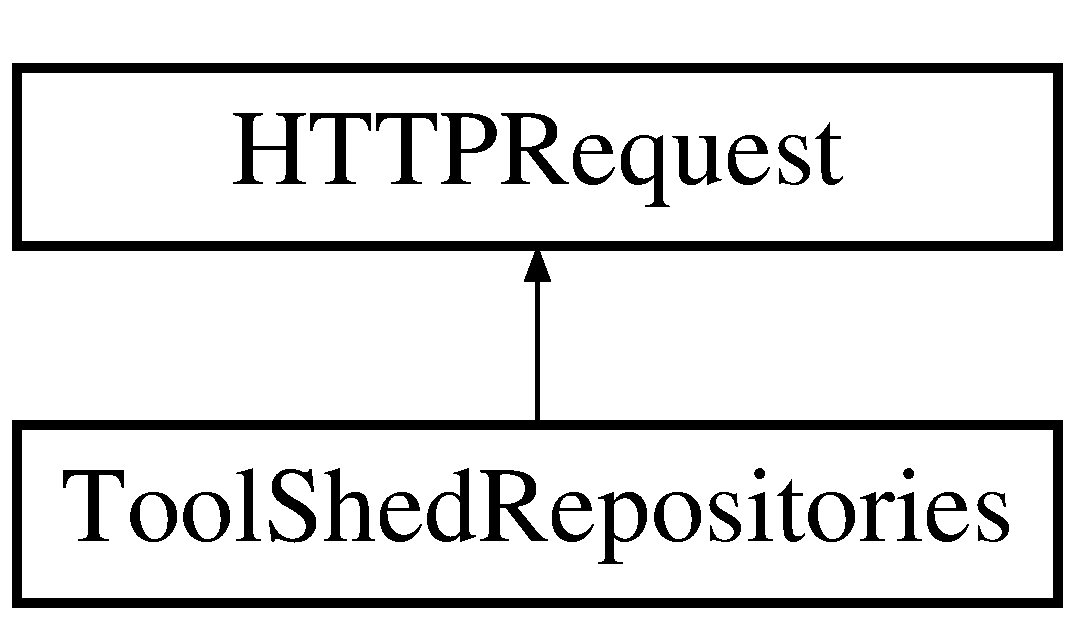
\includegraphics[height=2.000000cm]{classToolShedRepositories}
\end{center}
\end{figure}
\subsection*{Public Member Functions}
\begin{DoxyCompactItemize}
\item 
\hyperlink{classToolShedRepositories_ab56e4a423edc1a5ed031c4c9577cc0ff}{\+\_\+\+\_\+construct} (\$galaxy)
\item 
\hyperlink{classToolShedRepositories_acb3980f17136e97d4fa59154cc244972}{exported\+Workflows} (\$tool\+\_\+shed\+\_\+repo\+\_\+id)
\item 
\hyperlink{classToolShedRepositories_a53d6bd1df455d24d3739a7899b4e7dc8}{get\+Latest\+Installable} (\$tool\+\_\+shed\+\_\+url, \$name\+\_\+of\+\_\+repo, \$owner\+\_\+of\+\_\+repo)
\item 
\hyperlink{classToolShedRepositories_a61346794a4621ded6a8e7e261e80a0bd}{import\+Workflow} (\$tool\+\_\+shed\+\_\+repo\+\_\+id, \$\hyperlink{classToolShedRepositories_a7876ffc1b34b68094bb09b5f485bef4f}{index}=0)
\item 
\hyperlink{classToolShedRepositories_a7876ffc1b34b68094bb09b5f485bef4f}{index} ()
\item 
\hyperlink{classToolShedRepositories_aed1040aa143e1625bf0edce49eb2b272}{install\+\_\+repository\+\_\+revision} (\$tool\+\_\+shed\+\_\+url, \$name\+\_\+of\+\_\+repo, \$name\+\_\+owner\+\_\+of\+\_\+repo, \$changeset\+\_\+revision, \$new\+\_\+tool\+\_\+panel\+\_\+section\+\_\+label=N\+U\+LL, \$tool\+\_\+panel\+\_\+section\+\_\+id=N\+U\+LL, \$install\+\_\+repo\+\_\+dependencies=F\+A\+L\+SE, \$shed\+\_\+tool\+\_\+conf=N\+U\+LL)
\item 
\hyperlink{classToolShedRepositories_ae38b97508575d84d60d4f30bc72dc314}{repair\+\_\+repository\+\_\+revision} (\$admin\+\_\+api\+\_\+key, \$tool\+\_\+shed\+\_\+url, \$name\+\_\+of\+\_\+repo, \$owner\+\_\+of\+\_\+repo, \$changeset\+\_\+revision)
\item 
\hyperlink{classToolShedRepositories_a29438f079b2fb983b66daad8a471b235}{reset\+\_\+metadata\+\_\+on\+\_\+installed\+\_\+repositories} (\$admin\+\_\+api\+\_\+key)
\end{DoxyCompactItemize}
\subsection*{Additional Inherited Members}


\subsection{Constructor \& Destructor Documentation}
\index{Tool\+Shed\+Repositories@{Tool\+Shed\+Repositories}!\+\_\+\+\_\+construct@{\+\_\+\+\_\+construct}}
\index{\+\_\+\+\_\+construct@{\+\_\+\+\_\+construct}!Tool\+Shed\+Repositories@{Tool\+Shed\+Repositories}}
\subsubsection[{\texorpdfstring{\+\_\+\+\_\+construct(\$galaxy)}{\_\_construct($galaxy)}}]{\setlength{\rightskip}{0pt plus 5cm}Tool\+Shed\+Repositories\+::\+\_\+\+\_\+construct (
\begin{DoxyParamCaption}
\item[{}]{\$galaxy}
\end{DoxyParamCaption}
)}\hypertarget{classToolShedRepositories_ab56e4a423edc1a5ed031c4c9577cc0ff}{}\label{classToolShedRepositories_ab56e4a423edc1a5ed031c4c9577cc0ff}
The \hyperlink{classTools}{Tools} constructor.


\begin{DoxyParams}[1]{Parameters}
\hyperlink{classGalaxyInstance}{Galaxy\+Instance} & {\em \$galaxy} & A \hyperlink{classGalaxyInstance}{Galaxy\+Instance} object.\\
\hline
\end{DoxyParams}
\begin{DoxyReturn}{Returns}
An instance of a Tool shed repositories object. 
\end{DoxyReturn}


\subsection{Member Function Documentation}
\index{Tool\+Shed\+Repositories@{Tool\+Shed\+Repositories}!exported\+Workflows@{exported\+Workflows}}
\index{exported\+Workflows@{exported\+Workflows}!Tool\+Shed\+Repositories@{Tool\+Shed\+Repositories}}
\subsubsection[{\texorpdfstring{exported\+Workflows(\$tool\+\_\+shed\+\_\+repo\+\_\+id)}{exportedWorkflows($tool\_shed\_repo\_id)}}]{\setlength{\rightskip}{0pt plus 5cm}Tool\+Shed\+Repositories\+::exported\+Workflows (
\begin{DoxyParamCaption}
\item[{}]{\$tool\+\_\+shed\+\_\+repo\+\_\+id}
\end{DoxyParamCaption}
)}\hypertarget{classToolShedRepositories_acb3980f17136e97d4fa59154cc244972}{}\label{classToolShedRepositories_acb3980f17136e97d4fa59154cc244972}
Displays a list of dictionaries containing information about this tool shed repository\textquotesingle{}s exported workflows

Corresponds to the Galaxy A\+P\+I/path at G\+ET /api/tool\+\_\+shed\+\_\+repositories/\{encoded\+\_\+tool\+\_\+shed\+\_\+repository\+\_\+id\}/ exported\+\_\+workflows


\begin{DoxyParams}{Parameters}
{\em \$tool\+\_\+shed\+\_\+repo\+\_\+id} & Encoded Tool Shed Repository object encoded ID. To obtain a tool shed repository id, please use this class\textquotesingle{}s \hyperlink{classToolShedRepositories_a7876ffc1b34b68094bb09b5f485bef4f}{index()} function.\\
\hline
\end{DoxyParams}
\begin{DoxyReturn}{Returns}
An array containing information about a tool shed repositorie\textquotesingle{}s exported workflow. 
\end{DoxyReturn}
\index{Tool\+Shed\+Repositories@{Tool\+Shed\+Repositories}!get\+Latest\+Installable@{get\+Latest\+Installable}}
\index{get\+Latest\+Installable@{get\+Latest\+Installable}!Tool\+Shed\+Repositories@{Tool\+Shed\+Repositories}}
\subsubsection[{\texorpdfstring{get\+Latest\+Installable(\$tool\+\_\+shed\+\_\+url, \$name\+\_\+of\+\_\+repo, \$owner\+\_\+of\+\_\+repo)}{getLatestInstallable($tool\_shed\_url, $name\_of\_repo, $owner\_of\_repo)}}]{\setlength{\rightskip}{0pt plus 5cm}Tool\+Shed\+Repositories\+::get\+Latest\+Installable (
\begin{DoxyParamCaption}
\item[{}]{\$tool\+\_\+shed\+\_\+url, }
\item[{}]{\$name\+\_\+of\+\_\+repo, }
\item[{}]{\$owner\+\_\+of\+\_\+repo}
\end{DoxyParamCaption}
)}\hypertarget{classToolShedRepositories_a53d6bd1df455d24d3739a7899b4e7dc8}{}\label{classToolShedRepositories_a53d6bd1df455d24d3739a7899b4e7dc8}
Get the latest installable revision of a specified repository from a specified Tool Shed.

Corresponds to the Galaxy A\+P\+I/path at P\+O\+ST /api/tool\+\_\+shed\+\_\+repositories/get\+\_\+latest\+\_\+installable\+\_\+revision


\begin{DoxyParams}{Parameters}
{\em \$tool\+\_\+shed\+\_\+url} & The U\+RL of the Tool Shed from which to retrieve the Repo revision This should be something similar to this\+: \href{https://toolshed.g2.bx.psu.edu/repository?repository_id=253e22fdaf6a52c1}{\tt https\+://toolshed.\+g2.\+bx.\+psu.\+edu/repository?repository\+\_\+id=253e22fdaf6a52c1} \\
\hline
{\em \$name\+\_\+of\+\_\+repo} & The name of the repository \\
\hline
{\em \$owner\+\_\+of\+\_\+repo} & The name of the owner of the repository\\
\hline
\end{DoxyParams}
\begin{DoxyReturn}{Returns}
A changeset\+\_\+revision hash yo (describes the revison \textquotesingle{}number\textquotesingle{} of the tool) i.\+e 1\+:7002b364c3f8 1 being the true rev. number (the larger the more changes it\textquotesingle{}s been through, behind the colon is a supposed unique hash string, though collisions happen) 
\end{DoxyReturn}
\index{Tool\+Shed\+Repositories@{Tool\+Shed\+Repositories}!import\+Workflow@{import\+Workflow}}
\index{import\+Workflow@{import\+Workflow}!Tool\+Shed\+Repositories@{Tool\+Shed\+Repositories}}
\subsubsection[{\texorpdfstring{import\+Workflow(\$tool\+\_\+shed\+\_\+repo\+\_\+id, \$index=0)}{importWorkflow($tool\_shed\_repo\_id, $index=0)}}]{\setlength{\rightskip}{0pt plus 5cm}Tool\+Shed\+Repositories\+::import\+Workflow (
\begin{DoxyParamCaption}
\item[{}]{\$tool\+\_\+shed\+\_\+repo\+\_\+id, }
\item[{}]{\$index = {\ttfamily 0}}
\end{DoxyParamCaption}
)}\hypertarget{classToolShedRepositories_a61346794a4621ded6a8e7e261e80a0bd}{}\label{classToolShedRepositories_a61346794a4621ded6a8e7e261e80a0bd}
Import the specified exported workflow contained in a tool shed repo.

Corresponds to the Galaxy A\+P\+I/method at P\+O\+ST /api/tool\+\_\+shed\+\_\+repositories/import\+\_\+workflow


\begin{DoxyParams}{Parameters}
{\em \$tool\+\_\+shed\+\_\+repo\+\_\+id} & The encoded id of the Tool Shed Repository object\\
\hline
{\em \$index} & The location of the workflow to import from within the specified toolshed, defaults to 0 \\
\hline
\end{DoxyParams}
\begin{DoxyReturn}{Returns}
An array containing informaiton of the imported workflow. 
\end{DoxyReturn}
\index{Tool\+Shed\+Repositories@{Tool\+Shed\+Repositories}!index@{index}}
\index{index@{index}!Tool\+Shed\+Repositories@{Tool\+Shed\+Repositories}}
\subsubsection[{\texorpdfstring{index()}{index()}}]{\setlength{\rightskip}{0pt plus 5cm}Tool\+Shed\+Repositories\+::index (
\begin{DoxyParamCaption}
{}
\end{DoxyParamCaption}
)}\hypertarget{classToolShedRepositories_a7876ffc1b34b68094bb09b5f485bef4f}{}\label{classToolShedRepositories_a7876ffc1b34b68094bb09b5f485bef4f}
Display metadata on external tool shed repositories in galaxy instance

Corresponds to the Galaxy A\+P\+I/path at G\+ET /api/tool\+\_\+shed\+\_\+repositories

\begin{DoxyReturn}{Returns}
Json containing metadata on remote toolsheds galaxy instance 
\end{DoxyReturn}
\index{Tool\+Shed\+Repositories@{Tool\+Shed\+Repositories}!install\+\_\+repository\+\_\+revision@{install\+\_\+repository\+\_\+revision}}
\index{install\+\_\+repository\+\_\+revision@{install\+\_\+repository\+\_\+revision}!Tool\+Shed\+Repositories@{Tool\+Shed\+Repositories}}
\subsubsection[{\texorpdfstring{install\+\_\+repository\+\_\+revision(\$tool\+\_\+shed\+\_\+url, \$name\+\_\+of\+\_\+repo, \$name\+\_\+owner\+\_\+of\+\_\+repo, \$changeset\+\_\+revision, \$new\+\_\+tool\+\_\+panel\+\_\+section\+\_\+label=\+N\+U\+L\+L, \$tool\+\_\+panel\+\_\+section\+\_\+id=\+N\+U\+L\+L, \$install\+\_\+repo\+\_\+dependencies=\+F\+A\+L\+S\+E, \$shed\+\_\+tool\+\_\+conf=\+N\+U\+L\+L)}{install\_repository\_revision($tool\_shed\_url, $name\_of\_repo, $name\_owner\_of\_repo, $changeset\_revision, $new\_tool\_panel\_section\_label=NULL, $tool\_panel\_section\_id=NULL, $install\_repo\_dependencies=FALSE, $shed\_tool\_conf=NULL)}}]{\setlength{\rightskip}{0pt plus 5cm}Tool\+Shed\+Repositories\+::install\+\_\+repository\+\_\+revision (
\begin{DoxyParamCaption}
\item[{}]{\$tool\+\_\+shed\+\_\+url, }
\item[{}]{\$name\+\_\+of\+\_\+repo, }
\item[{}]{\$name\+\_\+owner\+\_\+of\+\_\+repo, }
\item[{}]{\$changeset\+\_\+revision, }
\item[{}]{\$new\+\_\+tool\+\_\+panel\+\_\+section\+\_\+label = {\ttfamily NULL}, }
\item[{}]{\$tool\+\_\+panel\+\_\+section\+\_\+id = {\ttfamily NULL}, }
\item[{}]{\$install\+\_\+repo\+\_\+dependencies = {\ttfamily FALSE}, }
\item[{}]{\$shed\+\_\+tool\+\_\+conf = {\ttfamily NULL}}
\end{DoxyParamCaption}
)}\hypertarget{classToolShedRepositories_aed1040aa143e1625bf0edce49eb2b272}{}\label{classToolShedRepositories_aed1040aa143e1625bf0edce49eb2b272}
Install a specified repository revision from a specified tool shed repo.

Corresponds to the Galaxy A\+P\+I/path P\+O\+ST /api/tool\+\_\+shed\+\_\+repositories/install\+\_\+repository\+\_\+revision


\begin{DoxyParams}{Parameters}
{\em \$tool\+\_\+shed\+\_\+url} & The base U\+RL of the Tool Shed from which to install the repo \\
\hline
{\em \$name\+\_\+of\+\_\+repo} & The name of the repository \\
\hline
{\em \$name\+\_\+owner\+\_\+of\+\_\+repo.} & The name of the owner of the repository \\
\hline
{\em \$changeset\+\_\+revision} & The changeset\+\_\+revision of the Repository Meta Data object associated with the Repository \\
\hline
{\em \$new\+\_\+tool\+\_\+panel\+\_\+section\+\_\+label} & (O\+P\+T\+I\+O\+N\+AL) Label of a new section to be added to the Galaxy tool panel in which to load tools contained in the Repository. Either this parameter must be an empty string or the tool\+\_\+panel\+\_\+section\+\_\+id paramter must be an empty string or both must be an empty string B\+O\+TH C\+A\+N\+N\+OT BE U\+S\+ED S\+I\+M\+U\+L\+T\+A\+N\+E\+O\+U\+S\+LY \\
\hline
{\em \$tool\+\_\+panel\+\_\+section\+\_\+id} & (O\+P\+T\+I\+O\+N\+AL) Id of the Galaxy tool panel section in which to load tools contained in the Repository. Either this parameter must be an empty string or the new\+\_\+tool\+\_\+panel\+\_\+section\+\_\+label paramter must be an empty string or both must be an empty string B\+O\+TH C\+A\+N\+N\+OT BE U\+S\+ED S\+I\+M\+U\+L\+T\+A\+N\+E\+O\+U\+S\+LY \\
\hline
{\em \$install\+\_\+repo\+\_\+dependencies} & (O\+P\+T\+I\+O\+N\+AL) Set to True if you want to install repository dependencies defined for the specified repository being installed. The default setting is False \\
\hline
{\em \$shed\+\_\+tool\+\_\+conf} & (O\+P\+T\+I\+O\+N\+AL) The shed-\/related tool panel configuration file configured in the \char`\"{}tool\+\_\+config\+\_\+file\char`\"{} setting in the Galaxy config file (ex\+: galaxy.\+ini). At least oneshed-\/reelated tool panel config file is required to be configured. Setting this paramter to a specific file enables you to choose where the specified repository wilel be installed because the tool\+\_\+path attribute of the $<$toolbox$>$ from the specified file is used as the installation location (ex\+: $<$toolbox tool\+\_\+path=\char`\"{}../shed\+\_\+tools\char`\"{}$>$). If this parameter is not set, a shed-\/related tool ppanel configuration file will be selected automatically \\
\hline
\end{DoxyParams}
\index{Tool\+Shed\+Repositories@{Tool\+Shed\+Repositories}!repair\+\_\+repository\+\_\+revision@{repair\+\_\+repository\+\_\+revision}}
\index{repair\+\_\+repository\+\_\+revision@{repair\+\_\+repository\+\_\+revision}!Tool\+Shed\+Repositories@{Tool\+Shed\+Repositories}}
\subsubsection[{\texorpdfstring{repair\+\_\+repository\+\_\+revision(\$admin\+\_\+api\+\_\+key, \$tool\+\_\+shed\+\_\+url, \$name\+\_\+of\+\_\+repo, \$owner\+\_\+of\+\_\+repo, \$changeset\+\_\+revision)}{repair\_repository\_revision($admin\_api\_key, $tool\_shed\_url, $name\_of\_repo, $owner\_of\_repo, $changeset\_revision)}}]{\setlength{\rightskip}{0pt plus 5cm}Tool\+Shed\+Repositories\+::repair\+\_\+repository\+\_\+revision (
\begin{DoxyParamCaption}
\item[{}]{\$admin\+\_\+api\+\_\+key, }
\item[{}]{\$tool\+\_\+shed\+\_\+url, }
\item[{}]{\$name\+\_\+of\+\_\+repo, }
\item[{}]{\$owner\+\_\+of\+\_\+repo, }
\item[{}]{\$changeset\+\_\+revision}
\end{DoxyParamCaption}
)}\hypertarget{classToolShedRepositories_ae38b97508575d84d60d4f30bc72dc314}{}\label{classToolShedRepositories_ae38b97508575d84d60d4f30bc72dc314}
Repair a specified repository revision previously installed into Galaxy

Corresponds to the Galaxy method/path P\+O\+ST /api/too\+\_\+sed\+\_\+repositories/repair\+\_\+repository\+\_\+revision


\begin{DoxyParams}{Parameters}
{\em \$admin\+\_\+api\+\_\+key} & The current Galaxy damin user\textquotesingle{}s A\+PI key \\
\hline
{\em \$tool\+\_\+shed\+\_\+url} & The base U\+RL of the Toool Shed from which the Repo was installed \\
\hline
{\em \$name\+\_\+of\+\_\+repo} & The name of the Repository \\
\hline
{\em \$owner\+\_\+of\+\_\+repo} & The owner of the Repository \\
\hline
{\em \$changeset\+\_\+revision} & The changeset\+\_\+revision of the Repository Meta data object associated with the Repository \\
\hline
\end{DoxyParams}
\index{Tool\+Shed\+Repositories@{Tool\+Shed\+Repositories}!reset\+\_\+metadata\+\_\+on\+\_\+installed\+\_\+repositories@{reset\+\_\+metadata\+\_\+on\+\_\+installed\+\_\+repositories}}
\index{reset\+\_\+metadata\+\_\+on\+\_\+installed\+\_\+repositories@{reset\+\_\+metadata\+\_\+on\+\_\+installed\+\_\+repositories}!Tool\+Shed\+Repositories@{Tool\+Shed\+Repositories}}
\subsubsection[{\texorpdfstring{reset\+\_\+metadata\+\_\+on\+\_\+installed\+\_\+repositories(\$admin\+\_\+api\+\_\+key)}{reset\_metadata\_on\_installed\_repositories($admin\_api\_key)}}]{\setlength{\rightskip}{0pt plus 5cm}Tool\+Shed\+Repositories\+::reset\+\_\+metadata\+\_\+on\+\_\+installed\+\_\+repositories (
\begin{DoxyParamCaption}
\item[{}]{\$admin\+\_\+api\+\_\+key}
\end{DoxyParamCaption}
)}\hypertarget{classToolShedRepositories_a29438f079b2fb983b66daad8a471b235}{}\label{classToolShedRepositories_a29438f079b2fb983b66daad8a471b235}
Resets all metadata on all repositories installed.

Corresponds to the Galaxy A\+P\+I/path P\+UT /api/tool\+\_\+shed\+\_\+repositories/reset\+\_\+metadata\+\_\+on\+\_\+installed\+\_\+repositories


\begin{DoxyParams}{Parameters}
{\em \$admin\+\_\+api\+\_\+key} & The current Galaxy damin user\textquotesingle{}s A\+PI key \\
\hline
\end{DoxyParams}


The documentation for this class was generated from the following file\+:\begin{DoxyCompactItemize}
\item 
\hyperlink{ToolShedRepositories_8inc}{Tool\+Shed\+Repositories.\+inc}\end{DoxyCompactItemize}

\hypertarget{classUsers}{}\section{Users Class Reference}
\label{classUsers}\index{Users@{Users}}
Inheritance diagram for Users\+:\begin{figure}[H]
\begin{center}
\leavevmode
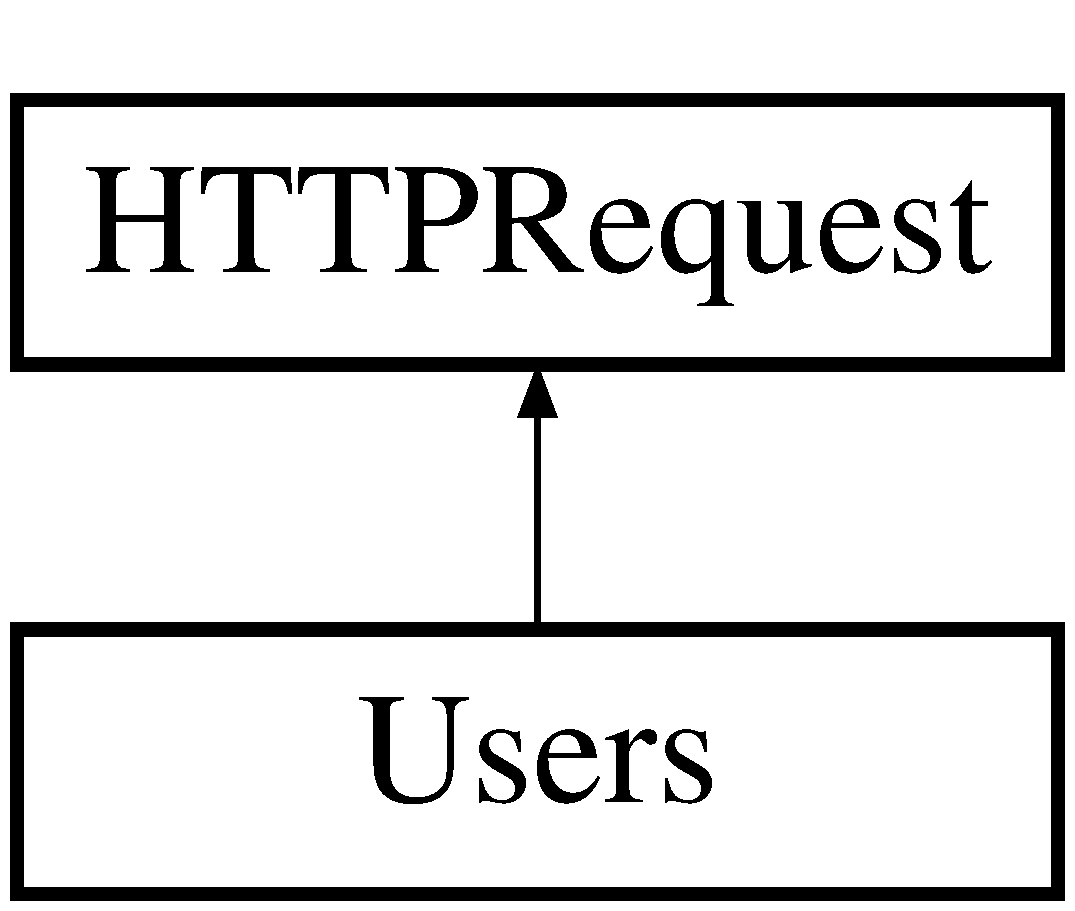
\includegraphics[height=2.000000cm]{classUsers}
\end{center}
\end{figure}
\subsection*{Public Member Functions}
\begin{DoxyCompactItemize}
\item 
\hyperlink{classUsers_a769aa9c30c6d94646c99f51807743c5c}{\+\_\+\+\_\+construct} (\$galaxy)
\item 
\hyperlink{classUsers_aae18145ee4c1d9b9eca0fd8e2d8d65d3}{index} (\$deleted=false, \$email=N\+U\+LL, \$username=N\+U\+LL, \$any=false)
\item 
\hyperlink{classUsers_a9c2cf59f933e4e59745351a7533ce0ab}{show} (\$user\+\_\+id)
\item 
\hyperlink{classUsers_a3169049c092532596a5d5c664f2d3fc5}{api\+Key} (\$user\+\_\+id)
\item 
\hyperlink{classUsers_a38f0657d88ec8be06dfc36c261b01814}{create} (\$username, \$user\+\_\+email, \$password)
\item 
\hyperlink{classUsers_a73e0c5b2dbcf185f32d9e72c3934e866}{update} ()
\item 
\hyperlink{classUsers_a84360c2388a75d4282a8aa789f13b982}{undelete} ()
\item 
\hyperlink{classUsers_aca99b21a27c17a7ee22546fc8145257d}{delete} (\$user\+\_\+id, \$purge=F\+A\+L\+SE)
\item 
\hyperlink{classUsers_a60cb5a1a81e5b7cdd9ca990d55f4624b}{get\+User\+ID} (\$username)
\end{DoxyCompactItemize}
\subsection*{Additional Inherited Members}


\subsection{Constructor \& Destructor Documentation}
\index{Users@{Users}!\+\_\+\+\_\+construct@{\+\_\+\+\_\+construct}}
\index{\+\_\+\+\_\+construct@{\+\_\+\+\_\+construct}!Users@{Users}}
\subsubsection[{\texorpdfstring{\+\_\+\+\_\+construct(\$galaxy)}{\_\_construct($galaxy)}}]{\setlength{\rightskip}{0pt plus 5cm}Users\+::\+\_\+\+\_\+construct (
\begin{DoxyParamCaption}
\item[{}]{\$galaxy}
\end{DoxyParamCaption}
)}\hypertarget{classUsers_a769aa9c30c6d94646c99f51807743c5c}{}\label{classUsers_a769aa9c30c6d94646c99f51807743c5c}
The \hyperlink{classUsers}{Users} constructor.


\begin{DoxyParams}[1]{Parameters}
\hyperlink{classGalaxyInstance}{Galaxy\+Instance} & {\em \$galaxy} & A \hyperlink{classGalaxyInstance}{Galaxy\+Instance} object.\\
\hline
\end{DoxyParams}
\begin{DoxyReturn}{Returns}
An instance of a \hyperlink{classUsers}{Users} object. 
\end{DoxyReturn}


\subsection{Member Function Documentation}
\index{Users@{Users}!api\+Key@{api\+Key}}
\index{api\+Key@{api\+Key}!Users@{Users}}
\subsubsection[{\texorpdfstring{api\+Key(\$user\+\_\+id)}{apiKey($user\_id)}}]{\setlength{\rightskip}{0pt plus 5cm}Users\+::api\+Key (
\begin{DoxyParamCaption}
\item[{}]{\$user\+\_\+id}
\end{DoxyParamCaption}
)}\hypertarget{classUsers_a3169049c092532596a5d5c664f2d3fc5}{}\label{classUsers_a3169049c092532596a5d5c664f2d3fc5}
Creates a new A\+PI key for specified user.

Corresponds to the Galaxy A\+P\+I/path P\+O\+ST /api/users/\{encoded\+\_\+user\+\_\+id\}/api\+\_\+key


\begin{DoxyParams}{Parameters}
{\em user\+\_\+id} & The id of the specified user. To obtain a user id, please use this class\textquotesingle{}s index function.\\
\hline
\end{DoxyParams}
\begin{DoxyReturn}{Returns}
The A\+PI key of the user. 
\end{DoxyReturn}
\index{Users@{Users}!create@{create}}
\index{create@{create}!Users@{Users}}
\subsubsection[{\texorpdfstring{create(\$username, \$user\+\_\+email, \$password)}{create($username, $user\_email, $password)}}]{\setlength{\rightskip}{0pt plus 5cm}Users\+::create (
\begin{DoxyParamCaption}
\item[{}]{\$username, }
\item[{}]{\$user\+\_\+email, }
\item[{}]{\$password}
\end{DoxyParamCaption}
)}\hypertarget{classUsers_a38f0657d88ec8be06dfc36c261b01814}{}\label{classUsers_a38f0657d88ec8be06dfc36c261b01814}
Creates new galaxy user.

Corresponds to the Galaxy A\+P\+I/path P\+O\+ST /api/users For this method to work, the Galaxy instance must have the allow\+\_\+user\+\_\+creation option set to True and use\+\_\+remote\+\_\+user option set to False in the config/galaxy.\+ini configuration file.


\begin{DoxyParams}{Parameters}
{\em username} & The username of the new user. \\
\hline
{\em user\+\_\+email} & The email of the new user. \\
\hline
{\em password} & The password of the new user.\\
\hline
\end{DoxyParams}
\begin{DoxyReturn}{Returns}
An array containing details of the new user. On failure F\+A\+L\+SE is returned. 
\end{DoxyReturn}
\index{Users@{Users}!delete@{delete}}
\index{delete@{delete}!Users@{Users}}
\subsubsection[{\texorpdfstring{delete(\$user\+\_\+id, \$purge=\+F\+A\+L\+S\+E)}{delete($user\_id, $purge=FALSE)}}]{\setlength{\rightskip}{0pt plus 5cm}Users\+::delete (
\begin{DoxyParamCaption}
\item[{}]{\$user\+\_\+id, }
\item[{}]{\$purge = {\ttfamily FALSE}}
\end{DoxyParamCaption}
)}\hypertarget{classUsers_aca99b21a27c17a7ee22546fc8145257d}{}\label{classUsers_aca99b21a27c17a7ee22546fc8145257d}
Mark a given user as deleted

Corresponds to the Galaxy A\+P\+I/path D\+E\+L\+E\+TE /api/users/\{id\}


\begin{DoxyParams}{Parameters}
{\em user\+\_\+id} & The id of the user to delete. To obtain a user id, please use this class\textquotesingle{}s index function. \\
\hline
{\em purge} & (Optional) if true, the user will be completely erased from Galaxy.\\
\hline
\end{DoxyParams}
\begin{DoxyReturn}{Returns}
An array containing details of the deleted user, or F\+A\+L\+SE on failure. 
\end{DoxyReturn}
\index{Users@{Users}!get\+User\+ID@{get\+User\+ID}}
\index{get\+User\+ID@{get\+User\+ID}!Users@{Users}}
\subsubsection[{\texorpdfstring{get\+User\+I\+D(\$username)}{getUserID($username)}}]{\setlength{\rightskip}{0pt plus 5cm}Users\+::get\+User\+ID (
\begin{DoxyParamCaption}
\item[{}]{\$username}
\end{DoxyParamCaption}
)}\hypertarget{classUsers_a60cb5a1a81e5b7cdd9ca990d55f4624b}{}\label{classUsers_a60cb5a1a81e5b7cdd9ca990d55f4624b}
Retrieves the ID of a Galaxy user.


\begin{DoxyParams}{Parameters}
{\em \$username} & The name of the user. \\
\hline
\end{DoxyParams}
\begin{DoxyReturn}{Returns}
A string containing the user ID or F\+A\+L\+SE if the user could not be found. 
\end{DoxyReturn}
\index{Users@{Users}!index@{index}}
\index{index@{index}!Users@{Users}}
\subsubsection[{\texorpdfstring{index(\$deleted=false, \$email=\+N\+U\+L\+L, \$username=\+N\+U\+L\+L, \$any=false)}{index($deleted=false, $email=NULL, $username=NULL, $any=false)}}]{\setlength{\rightskip}{0pt plus 5cm}Users\+::index (
\begin{DoxyParamCaption}
\item[{}]{\$deleted = {\ttfamily false}, }
\item[{}]{\$email = {\ttfamily NULL}, }
\item[{}]{\$username = {\ttfamily NULL}, }
\item[{}]{\$any = {\ttfamily false}}
\end{DoxyParamCaption}
)}\hypertarget{classUsers_aae18145ee4c1d9b9eca0fd8e2d8d65d3}{}\label{classUsers_aae18145ee4c1d9b9eca0fd8e2d8d65d3}
Displays a collection of Galaxy users.

Corresponds to the Galaxy A\+P\+I/paths at G\+ET /api/users and G\+ET /api/users/deleted


\begin{DoxyParams}{Parameters}
{\em deleted} & (optional) If true, show deleted users. \\
\hline
{\em email} & (optional) An email address to filter results based on. \\
\hline
{\em name} & (optional) A username to filter results based on. \\
\hline
{\em any} & (optional) If true, Filter on username OR email.\\
\hline
\end{DoxyParams}
\begin{DoxyReturn}{Returns}
An array containing information on the the users the A\+PI function retreived 
\end{DoxyReturn}
\index{Users@{Users}!show@{show}}
\index{show@{show}!Users@{Users}}
\subsubsection[{\texorpdfstring{show(\$user\+\_\+id)}{show($user\_id)}}]{\setlength{\rightskip}{0pt plus 5cm}Users\+::show (
\begin{DoxyParamCaption}
\item[{}]{\$user\+\_\+id}
\end{DoxyParamCaption}
)}\hypertarget{classUsers_a9c2cf59f933e4e59745351a7533ce0ab}{}\label{classUsers_a9c2cf59f933e4e59745351a7533ce0ab}
Retreive detailed information on a specific user.

Corresponds to the Galaxy A\+P\+I/path G\+ET /api/users/\{encoded\+\_\+user\+\_\+id\}


\begin{DoxyParams}{Parameters}
{\em user\+\_\+id} & The id of the user whos details to retreive. To obtain a user id please use this class\textquotesingle{}s \hyperlink{classUsers_aae18145ee4c1d9b9eca0fd8e2d8d65d3}{index()} function.\\
\hline
\end{DoxyParams}
\begin{DoxyReturn}{Returns}
An array containing the details of the user. 
\end{DoxyReturn}
\index{Users@{Users}!undelete@{undelete}}
\index{undelete@{undelete}!Users@{Users}}
\subsubsection[{\texorpdfstring{undelete()}{undelete()}}]{\setlength{\rightskip}{0pt plus 5cm}Users\+::undelete (
\begin{DoxyParamCaption}
{}
\end{DoxyParamCaption}
)}\hypertarget{classUsers_a84360c2388a75d4282a8aa789f13b982}{}\label{classUsers_a84360c2388a75d4282a8aa789f13b982}
The actual python implementation is not complete \index{Users@{Users}!update@{update}}
\index{update@{update}!Users@{Users}}
\subsubsection[{\texorpdfstring{update()}{update()}}]{\setlength{\rightskip}{0pt plus 5cm}Users\+::update (
\begin{DoxyParamCaption}
{}
\end{DoxyParamCaption}
)}\hypertarget{classUsers_a73e0c5b2dbcf185f32d9e72c3934e866}{}\label{classUsers_a73e0c5b2dbcf185f32d9e72c3934e866}
The actual python implementation is not complete 

The documentation for this class was generated from the following file\+:\begin{DoxyCompactItemize}
\item 
\hyperlink{Users_8inc}{Users.\+inc}\end{DoxyCompactItemize}

\hypertarget{classVisualizations}{}\section{Visualizations Class Reference}
\label{classVisualizations}\index{Visualizations@{Visualizations}}
Inheritance diagram for Visualizations\+:\begin{figure}[H]
\begin{center}
\leavevmode
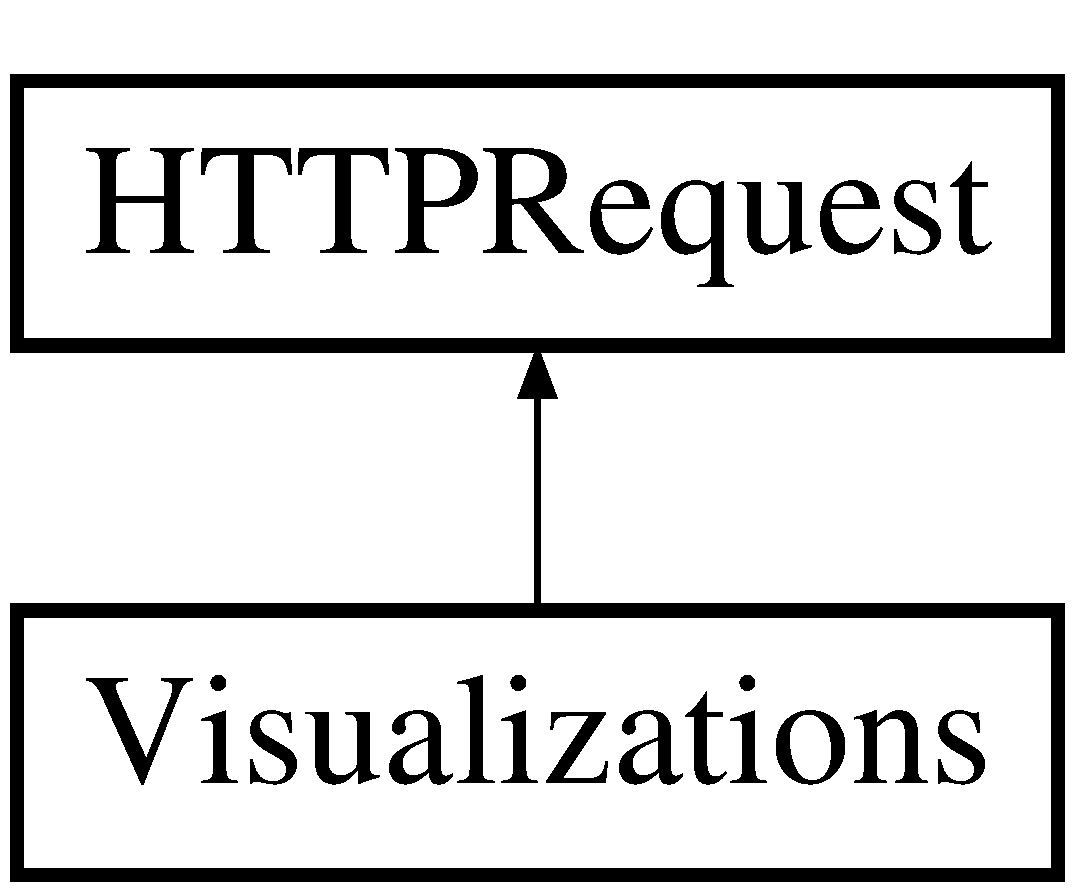
\includegraphics[height=2.000000cm]{classVisualizations}
\end{center}
\end{figure}
\subsection*{Public Member Functions}
\begin{DoxyCompactItemize}
\item 
\hyperlink{classVisualizations_a718efd55867c65bbd67f6c9bb4c3803b}{\+\_\+\+\_\+construct} (\$galaxy)
\item 
\hyperlink{classVisualizations_ad5f186b859ab85b4246604fa28671c77}{index} ()
\item 
\hyperlink{classVisualizations_a21c55eeee76f2d68990382405159e908}{show} (\$viz\+\_\+id)
\item 
\hyperlink{classVisualizations_a8d6b51b5d14c79e698ce118ad05eb995}{create} (\$type, \$title, \$dbkey, \$import\+\_\+id=N\+U\+LL)
\item 
\hyperlink{classVisualizations_aed3835f460ec550d7e6128e43b7e2241}{update} (\$viz\+\_\+id, \$title=null, \$dbkey=null, \$config=null)
\end{DoxyCompactItemize}
\subsection*{Additional Inherited Members}


\subsection{Constructor \& Destructor Documentation}
\index{Visualizations@{Visualizations}!\+\_\+\+\_\+construct@{\+\_\+\+\_\+construct}}
\index{\+\_\+\+\_\+construct@{\+\_\+\+\_\+construct}!Visualizations@{Visualizations}}
\subsubsection[{\texorpdfstring{\+\_\+\+\_\+construct(\$galaxy)}{\_\_construct($galaxy)}}]{\setlength{\rightskip}{0pt plus 5cm}Visualizations\+::\+\_\+\+\_\+construct (
\begin{DoxyParamCaption}
\item[{}]{\$galaxy}
\end{DoxyParamCaption}
)}\hypertarget{classVisualizations_a718efd55867c65bbd67f6c9bb4c3803b}{}\label{classVisualizations_a718efd55867c65bbd67f6c9bb4c3803b}
The visualizations constructor.


\begin{DoxyParams}[1]{Parameters}
\hyperlink{classGalaxyInstance}{Galaxy\+Instance} & {\em \$galaxy} & A \hyperlink{classGalaxyInstance}{Galaxy\+Instance} object\\
\hline
\end{DoxyParams}
\begin{DoxyReturn}{Returns}
An instance of a \hyperlink{classVisualizations}{Visualizations} object 
\end{DoxyReturn}


\subsection{Member Function Documentation}
\index{Visualizations@{Visualizations}!create@{create}}
\index{create@{create}!Visualizations@{Visualizations}}
\subsubsection[{\texorpdfstring{create(\$type, \$title, \$dbkey, \$import\+\_\+id=\+N\+U\+L\+L)}{create($type, $title, $dbkey, $import\_id=NULL)}}]{\setlength{\rightskip}{0pt plus 5cm}Visualizations\+::create (
\begin{DoxyParamCaption}
\item[{}]{\$type, }
\item[{}]{\$title, }
\item[{}]{\$dbkey, }
\item[{}]{\$import\+\_\+id = {\ttfamily NULL}}
\end{DoxyParamCaption}
)}\hypertarget{classVisualizations_a8d6b51b5d14c79e698ce118ad05eb995}{}\label{classVisualizations_a8d6b51b5d14c79e698ce118ad05eb995}
Imports copy of existing visualizatiion into the workplace.

Corresponds to the Galaxy A\+P\+I/paths at P\+O\+ST /api/visualizations or P\+O\+ST /api/visualizations?import\+\_\+id=\{encoded\+\_\+visualization\+\_\+id\}


\begin{DoxyParams}{Parameters}
{\em type} & The visualization type for the new visualization. \\
\hline
{\em title} & The title for the visualization. \\
\hline
{\em import\+\_\+id} & (optional)The id of the visualization to import, if the user desires to import a visualization.\\
\hline
\end{DoxyParams}
\begin{DoxyReturn}{Returns}
An array containing the created visualization. 
\end{DoxyReturn}
\index{Visualizations@{Visualizations}!index@{index}}
\index{index@{index}!Visualizations@{Visualizations}}
\subsubsection[{\texorpdfstring{index()}{index()}}]{\setlength{\rightskip}{0pt plus 5cm}Visualizations\+::index (
\begin{DoxyParamCaption}
{}
\end{DoxyParamCaption}
)}\hypertarget{classVisualizations_ad5f186b859ab85b4246604fa28671c77}{}\label{classVisualizations_ad5f186b859ab85b4246604fa28671c77}
Retreive a list of all visualizations.

Corresponds to the Galaxy A\+P\+I/path G\+ET /api/visualizations

\begin{DoxyReturn}{Returns}
An array containing all of galaxy\textquotesingle{}s visualizations. 
\end{DoxyReturn}
\index{Visualizations@{Visualizations}!show@{show}}
\index{show@{show}!Visualizations@{Visualizations}}
\subsubsection[{\texorpdfstring{show(\$viz\+\_\+id)}{show($viz\_id)}}]{\setlength{\rightskip}{0pt plus 5cm}Visualizations\+::show (
\begin{DoxyParamCaption}
\item[{}]{\$viz\+\_\+id}
\end{DoxyParamCaption}
)}\hypertarget{classVisualizations_a21c55eeee76f2d68990382405159e908}{}\label{classVisualizations_a21c55eeee76f2d68990382405159e908}
Retreive detailed information about a specific visualization.

Corresponds to the Galaxy A\+P\+I/path G\+ET /api/visualizations/$<$viz\+\_\+id$>$


\begin{DoxyParams}{Parameters}
{\em viz\+\_\+id} & The visualization id whos details to display. \\
\hline
\end{DoxyParams}
\index{Visualizations@{Visualizations}!update@{update}}
\index{update@{update}!Visualizations@{Visualizations}}
\subsubsection[{\texorpdfstring{update(\$viz\+\_\+id, \$title=null, \$dbkey=null, \$config=null)}{update($viz\_id, $title=null, $dbkey=null, $config=null)}}]{\setlength{\rightskip}{0pt plus 5cm}Visualizations\+::update (
\begin{DoxyParamCaption}
\item[{}]{\$viz\+\_\+id, }
\item[{}]{\$title = {\ttfamily null}, }
\item[{}]{\$dbkey = {\ttfamily null}, }
\item[{}]{\$config = {\ttfamily null}}
\end{DoxyParamCaption}
)}\hypertarget{classVisualizations_aed3835f460ec550d7e6128e43b7e2241}{}\label{classVisualizations_aed3835f460ec550d7e6128e43b7e2241}
Update a specific visualization

Corresponds to the Galaxy A\+P\+I/path at P\+UT /api/visualizations/$<$visualizations id$>$=\char`\"{}\char`\"{}$>$


\begin{DoxyParams}{Parameters}
{\em viz\+\_\+id} & visualization id of the visualization to update. To obtain this id please use this class\textquotesingle{}s index method. \\
\hline
{\em title} & If the user is changing the title, include the new title. \\
\hline
{\em \$dbkey} & If the user is changing the new db key, include the new dbkey. \\
\hline
{\em \$config} & The configuration of the visualization.\\
\hline
\end{DoxyParams}
\begin{DoxyReturn}{Returns}
An array containing the updated visualizaiton. 
\end{DoxyReturn}


The documentation for this class was generated from the following file\+:\begin{DoxyCompactItemize}
\item 
\hyperlink{Visualizations_8inc}{Visualizations.\+inc}\end{DoxyCompactItemize}

\hypertarget{classWorkflows}{}\section{Workflows Class Reference}
\label{classWorkflows}\index{Workflows@{Workflows}}
Inheritance diagram for Workflows\+:\begin{figure}[H]
\begin{center}
\leavevmode
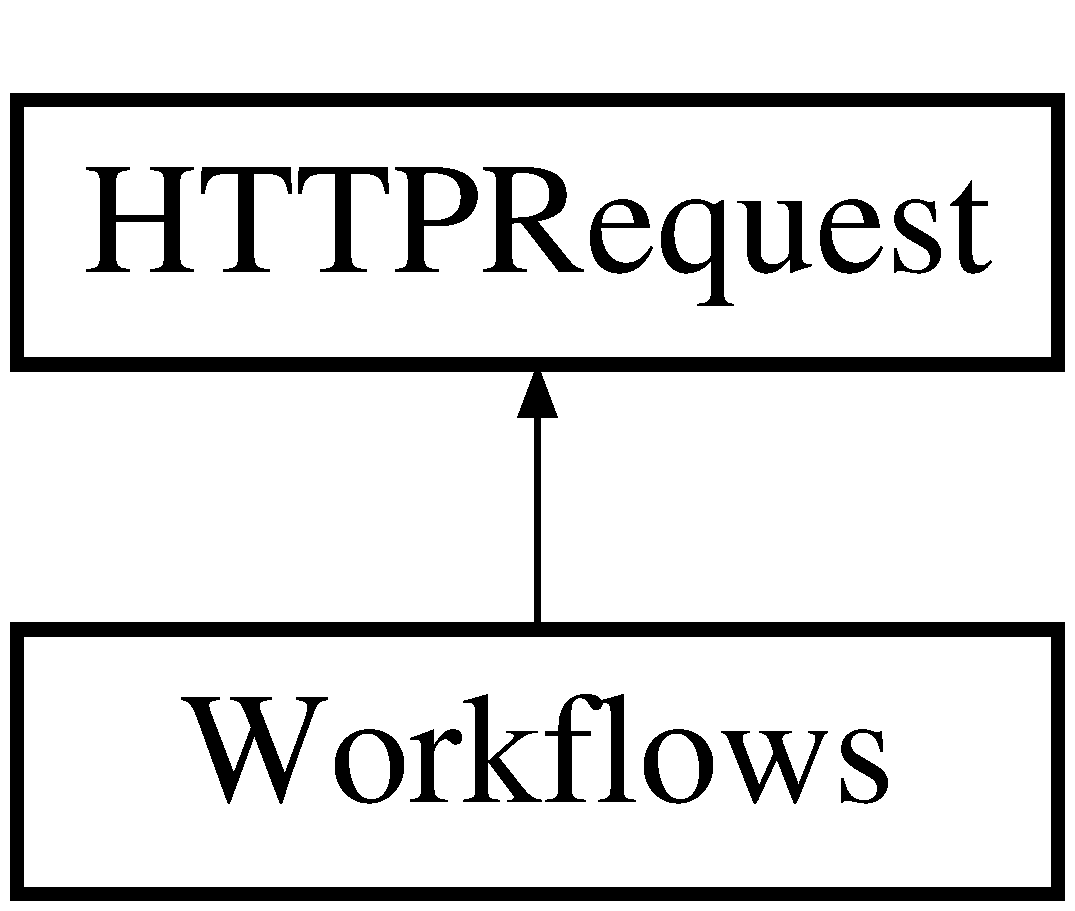
\includegraphics[height=2.000000cm]{classWorkflows}
\end{center}
\end{figure}
\subsection*{Public Member Functions}
\begin{DoxyCompactItemize}
\item 
\hyperlink{classWorkflows_acc3b406c5521cc768ad9aca9981f12f9}{\+\_\+\+\_\+construct} (\$galaxy)
\item 
\hyperlink{classWorkflows_ad111397f29f01809c4d803a7052075a7}{index} (\$is\+\_\+published=F\+A\+L\+SE)
\item 
\hyperlink{classWorkflows_abcd6e69e5f6fb77b5476c2303dda0a28}{show} (\$workflow\+\_\+id, \$show\+\_\+published=true)
\item 
\hyperlink{classWorkflows_a02d170de2fc5922195c37bcbd40c7fc3}{delete} (\$workflow\+\_\+id)
\item 
\hyperlink{classWorkflows_ab1d1388da67119d248dcb8cb38c48185}{export} (\$workflow\+\_\+id)
\item 
\hyperlink{classWorkflows_a4eb19053303e1c5e12ea7abd2de5718c}{download} (\$workflow\+\_\+id)
\item 
\hyperlink{classWorkflows_a2714dee5cc591b4bff8618ceccc9dbb2}{update} (\$workflow\+\_\+id, \$J\+S\+O\+N\+\_\+\+Workflow)
\item 
\hyperlink{classWorkflows_a6041804173008fa38f878265dde14405}{build\+Module} (\$tool\+\_\+id, \$tool\+\_\+input\+\_\+ids=N\+U\+LL, \$tool\+\_\+version=N\+U\+LL, \$annotation=N\+U\+LL)
\item 
\hyperlink{classWorkflows_a83c6891fd0b71d69917ad4dc0e2517d5}{index\+Invocations} (\$workflow\+\_\+id)
\item 
\hyperlink{classWorkflows_a3dfd3d41b78c18c112ebeab8bac7f6cf}{show\+Invocations} (\$workflow\+\_\+id, \$invocation\+\_\+id)
\item 
\hyperlink{classWorkflows_a51ecb7843d3ae01aaa080e56b3dd4be7}{cancel\+Invocation} (\$workflow\+\_\+id, \$invocation\+\_\+id)
\item 
\hyperlink{classWorkflows_a4a361f883c4e6f8d2dde77117de6e1c6}{invocation\+Steps} (\$workflow\+\_\+id, \$invocation\+\_\+id, \$step\+\_\+id)
\item 
\hyperlink{classWorkflows_a5dbf5a6dc6156664d6588b22599eebc5}{update\+Invocation\+Steps} (\$workflow\+\_\+id, \$invocation\+\_\+id, \$step\+\_\+id, \$payload=array())
\item 
\hyperlink{classWorkflows_a7e32dbe325c4d397e94da462fa71494f}{invoke} (\$workflow\+\_\+id, \$input\+\_\+dataset\+\_\+ids, \$parameters=N\+U\+LL, \$hist\+\_\+id=N\+U\+LL)
\item 
\hyperlink{classWorkflows_adec30fe8a3d234e40d257b5d917c079e}{create} (\$params)
\end{DoxyCompactItemize}
\subsection*{Additional Inherited Members}


\subsection{Constructor \& Destructor Documentation}
\index{Workflows@{Workflows}!\+\_\+\+\_\+construct@{\+\_\+\+\_\+construct}}
\index{\+\_\+\+\_\+construct@{\+\_\+\+\_\+construct}!Workflows@{Workflows}}
\subsubsection[{\texorpdfstring{\+\_\+\+\_\+construct(\$galaxy)}{\_\_construct($galaxy)}}]{\setlength{\rightskip}{0pt plus 5cm}Workflows\+::\+\_\+\+\_\+construct (
\begin{DoxyParamCaption}
\item[{}]{\$galaxy}
\end{DoxyParamCaption}
)}\hypertarget{classWorkflows_acc3b406c5521cc768ad9aca9981f12f9}{}\label{classWorkflows_acc3b406c5521cc768ad9aca9981f12f9}
The \hyperlink{classWorkflows}{Workflows} constructor.


\begin{DoxyParams}[1]{Parameters}
\hyperlink{classGalaxyInstance}{Galaxy\+Instance} & {\em \$galaxy} & A \hyperlink{classGalaxyInstance}{Galaxy\+Instance} object.\\
\hline
\end{DoxyParams}
\begin{DoxyReturn}{Returns}
An instance of a workflows object. 
\end{DoxyReturn}


\subsection{Member Function Documentation}
\index{Workflows@{Workflows}!build\+Module@{build\+Module}}
\index{build\+Module@{build\+Module}!Workflows@{Workflows}}
\subsubsection[{\texorpdfstring{build\+Module(\$tool\+\_\+id, \$tool\+\_\+input\+\_\+ids=\+N\+U\+L\+L, \$tool\+\_\+version=\+N\+U\+L\+L, \$annotation=\+N\+U\+L\+L)}{buildModule($tool\_id, $tool\_input\_ids=NULL, $tool\_version=NULL, $annotation=NULL)}}]{\setlength{\rightskip}{0pt plus 5cm}Workflows\+::build\+Module (
\begin{DoxyParamCaption}
\item[{}]{\$tool\+\_\+id, }
\item[{}]{\$tool\+\_\+input\+\_\+ids = {\ttfamily NULL}, }
\item[{}]{\$tool\+\_\+version = {\ttfamily NULL}, }
\item[{}]{\$annotation = {\ttfamily NULL}}
\end{DoxyParamCaption}
)}\hypertarget{classWorkflows_a6041804173008fa38f878265dde14405}{}\label{classWorkflows_a6041804173008fa38f878265dde14405}
T\+O\+DO incomplete \index{Workflows@{Workflows}!cancel\+Invocation@{cancel\+Invocation}}
\index{cancel\+Invocation@{cancel\+Invocation}!Workflows@{Workflows}}
\subsubsection[{\texorpdfstring{cancel\+Invocation(\$workflow\+\_\+id, \$invocation\+\_\+id)}{cancelInvocation($workflow\_id, $invocation\_id)}}]{\setlength{\rightskip}{0pt plus 5cm}Workflows\+::cancel\+Invocation (
\begin{DoxyParamCaption}
\item[{}]{\$workflow\+\_\+id, }
\item[{}]{\$invocation\+\_\+id}
\end{DoxyParamCaption}
)}\hypertarget{classWorkflows_a51ecb7843d3ae01aaa080e56b3dd4be7}{}\label{classWorkflows_a51ecb7843d3ae01aaa080e56b3dd4be7}
Cancel an invocation request.

Corresponds to the Galaxy A\+P\+I/path at D\+E\+L\+E\+TE /api/workflows/\{workflow\+\_\+id\}/invocation/\{invocation\+\_\+id\}


\begin{DoxyParams}{Parameters}
{\em workflow\+\_\+id} & The id of the workflow that the invocation belongs to. To obtain a workflow invocation, please use this class\textquotesingle{}s \hyperlink{classWorkflows_ad111397f29f01809c4d803a7052075a7}{index()} function. \\
\hline
{\em invocation\+\_\+id} & The id of the invocation to invoke.\\
\hline
\end{DoxyParams}
\begin{DoxyReturn}{Returns}
An array containing details of the specified invocation. 
\end{DoxyReturn}
\index{Workflows@{Workflows}!create@{create}}
\index{create@{create}!Workflows@{Workflows}}
\subsubsection[{\texorpdfstring{create(\$params)}{create($params)}}]{\setlength{\rightskip}{0pt plus 5cm}Workflows\+::create (
\begin{DoxyParamCaption}
\item[{}]{\$params}
\end{DoxyParamCaption}
)}\hypertarget{classWorkflows_adec30fe8a3d234e40d257b5d917c079e}{}\label{classWorkflows_adec30fe8a3d234e40d257b5d917c079e}
Creates or edits a workflow with the given parameters.

Corresponds to the Galaxy api/path at P\+O\+ST /api/workflows


\begin{DoxyParams}{Parameters}
{\em \$params} & A key value (associative array) where the keys can be the following\+:\\
\hline
\end{DoxyParams}
If importing a J\+S\+ON workflow\+:
\begin{DoxyItemize}
\item workflow\+: A J\+S\+ON representation of a workflow to be inserted into the database.
\end{DoxyItemize}

If running workflow from pre-\/existing workflow\+:
\begin{DoxyItemize}
\item workflow\+\_\+id\+: An existing workflow id. Either workflow\+\_\+id, installed\+\_\+repository\+\_\+file or from\+\_\+history\+\_\+id must be specified. To obtain a workflow id, please see this class\textquotesingle{}s \hyperlink{classWorkflows_ad111397f29f01809c4d803a7052075a7}{index()} function.
\item parameters\+: If workflow\+\_\+id is set, specify the parameters for the workflow. See this class\textquotesingle{}s \hyperlink{classWorkflows_a7e32dbe325c4d397e94da462fa71494f}{invoke()} for more details.
\item ds\+\_\+map\+: If workflow\+\_\+id is set -\/ a dictionary mapping each input step id to a dictionary with 2 keys\+: ‘src’ (which can be ‘ldda’, ‘ld’ or ‘hda’) and ‘id’ (which should be the id of a Library\+Dataset\+Dataset\+Association, Library\+Dataset or History\+Dataset\+Association respectively).
\item no\+\_\+add\+\_\+to\+\_\+history\+: If workflow\+\_\+id is set; if present in the payload with any value, the input datasets will not be added to the selected history.
\item replacement\+\_\+params\+: If workflow\+\_\+id is set an optional dictionary used when renaming datasets.
\item history\+: If workflow\+\_\+id is set optional history where to run the workflow, either the name of a new history or “hist\+\_\+id=H\+I\+S\+T\+\_\+\+I\+D” where H\+I\+S\+T\+\_\+\+ID is the id of an existing history. If not specified, the workflow will be run a new unnamed history. To obtain a history ID Please refer to the \hyperlink{classWorkflows_ad111397f29f01809c4d803a7052075a7}{index()} function in the histories class.
\end{DoxyItemize}

If Creating / Running workflows from a History
\begin{DoxyItemize}
\item from\+\_\+history\+\_\+id\+: Id of history to extract a workflow from. Either workflow\+\_\+id, installed\+\_\+repository\+\_\+file or from\+\_\+history\+\_\+id must be specified.
\item job\+\_\+ids\+: If from\+\_\+history\+\_\+id is set, optional list of jobs to include when extracting a workflow from history.
\item dataset\+\_\+collection\+\_\+ids\+: If from\+\_\+history\+\_\+id is set -\/ optional list of H\+D\+CA hid`s corresponding to workflow inputs when extracting a workflow from history.
\item workflow\+\_\+name\+: If from\+\_\+history\+\_\+id is set; name of the workflow to create when extracting a workflow from history.
\item allow\+\_\+tool\+\_\+state\+\_\+corrections\+: if set to True, any Tool parameter changes will not prevent running workflow, defaults to False.
\end{DoxyItemize}

\begin{DoxyReturn}{Returns}
An array containing the created workflow. 
\end{DoxyReturn}
\index{Workflows@{Workflows}!delete@{delete}}
\index{delete@{delete}!Workflows@{Workflows}}
\subsubsection[{\texorpdfstring{delete(\$workflow\+\_\+id)}{delete($workflow\_id)}}]{\setlength{\rightskip}{0pt plus 5cm}Workflows\+::delete (
\begin{DoxyParamCaption}
\item[{}]{\$workflow\+\_\+id}
\end{DoxyParamCaption}
)}\hypertarget{classWorkflows_a02d170de2fc5922195c37bcbd40c7fc3}{}\label{classWorkflows_a02d170de2fc5922195c37bcbd40c7fc3}
Delete a specified workflow.

Corresponds to the Galaxy A\+P\+I/method at D\+E\+L\+E\+TE /api/workflows/\{encoded\+\_\+workflow\+\_\+id\}


\begin{DoxyParams}{Parameters}
{\em \$workflow\+\_\+id} & The id of the workflow to delete. To obtain a workflow id please use this class\textquotesingle{}s index function. \\
\hline
\end{DoxyParams}
\index{Workflows@{Workflows}!download@{download}}
\index{download@{download}!Workflows@{Workflows}}
\subsubsection[{\texorpdfstring{download(\$workflow\+\_\+id)}{download($workflow\_id)}}]{\setlength{\rightskip}{0pt plus 5cm}Workflows\+::download (
\begin{DoxyParamCaption}
\item[{}]{\$workflow\+\_\+id}
\end{DoxyParamCaption}
)}\hypertarget{classWorkflows_a4eb19053303e1c5e12ea7abd2de5718c}{}\label{classWorkflows_a4eb19053303e1c5e12ea7abd2de5718c}
Returns a selected workflow (using a filepath) to download. It is similar to export except the returned J\+S\+ON does no include a \textquotesingle{}inputs\textquotesingle{} field.

Corresponds to the Galaxy A\+P\+I/path G\+ET /api/workflows/\{encoded\+\_\+workflow\+\_\+id\}/download


\begin{DoxyParams}{Parameters}
{\em \$workflow\+\_\+id} & Id of the Workflow to retreive To obtain a workflow id, please use this class \hyperlink{classWorkflows_ad111397f29f01809c4d803a7052075a7}{index()} function. \\
\hline
{\em \$file\+\_\+local\+\_\+path} & Local Path to which the exported file will be saved. (Should not contain filename if use\+\_\+default\+\_\+name=True). It must be the full path to which the object is to be saved \\
\hline
{\em \$use\+\_\+default\+\_\+filename} & If the use\+\_\+default\+\_\+name parameter is True, the exported file will be saved as file\+\_\+local\+\_\+path/\+Galaxy-\/\+Workflow-\/s.\+ga, where s is the workflow name. If use\+\_\+default\+\_\+name is False, file\+\_\+local\+\_\+path is assumed to contain the full file path including filename.\\
\hline
\end{DoxyParams}
\begin{DoxyReturn}{Returns}
An array of the selected workflow. 
\end{DoxyReturn}
\index{Workflows@{Workflows}!export@{export}}
\index{export@{export}!Workflows@{Workflows}}
\subsubsection[{\texorpdfstring{export(\$workflow\+\_\+id)}{export($workflow\_id)}}]{\setlength{\rightskip}{0pt plus 5cm}Workflows\+::export (
\begin{DoxyParamCaption}
\item[{}]{\$workflow\+\_\+id}
\end{DoxyParamCaption}
)}\hypertarget{classWorkflows_ab1d1388da67119d248dcb8cb38c48185}{}\label{classWorkflows_ab1d1388da67119d248dcb8cb38c48185}
Exports a workflow


\begin{DoxyParams}{Parameters}
{\em \$workflow\+\_\+id} & Encoded workflow ID.\\
\hline
\end{DoxyParams}
\begin{DoxyReturn}{Returns}
An array representing the workflow requested. 
\end{DoxyReturn}
\index{Workflows@{Workflows}!index@{index}}
\index{index@{index}!Workflows@{Workflows}}
\subsubsection[{\texorpdfstring{index(\$is\+\_\+published=\+F\+A\+L\+S\+E)}{index($is\_published=FALSE)}}]{\setlength{\rightskip}{0pt plus 5cm}Workflows\+::index (
\begin{DoxyParamCaption}
\item[{}]{\$is\+\_\+published = {\ttfamily FALSE}}
\end{DoxyParamCaption}
)}\hypertarget{classWorkflows_ad111397f29f01809c4d803a7052075a7}{}\label{classWorkflows_ad111397f29f01809c4d803a7052075a7}
Retreive a list of all the workflows.

Corresponds to the Galaxy A\+P\+I/path at G\+ET /api/workflows


\begin{DoxyParams}{Parameters}
{\em is\+\_\+published} & Optional, if true, published workflows will be displayed.\\
\hline
\end{DoxyParams}
\begin{DoxyReturn}{Returns}
An array containing all of the workflows in Galaxy. 
\end{DoxyReturn}
\index{Workflows@{Workflows}!index\+Invocations@{index\+Invocations}}
\index{index\+Invocations@{index\+Invocations}!Workflows@{Workflows}}
\subsubsection[{\texorpdfstring{index\+Invocations(\$workflow\+\_\+id)}{indexInvocations($workflow\_id)}}]{\setlength{\rightskip}{0pt plus 5cm}Workflows\+::index\+Invocations (
\begin{DoxyParamCaption}
\item[{}]{\$workflow\+\_\+id}
\end{DoxyParamCaption}
)}\hypertarget{classWorkflows_a83c6891fd0b71d69917ad4dc0e2517d5}{}\label{classWorkflows_a83c6891fd0b71d69917ad4dc0e2517d5}
Retreive a list of the workflow invocations for a given workflow.

Corresponds to the Galaxy A\+P\+I/path G\+ET /api/workflows/\{workflow\+\_\+id\}/invocations


\begin{DoxyParams}{Parameters}
{\em workflow\+\_\+id} & The id of the workflow whos invocations to retreive.\\
\hline
\end{DoxyParams}
\begin{DoxyReturn}{Returns}
An array containing the invocations of a workflow. 
\end{DoxyReturn}
\index{Workflows@{Workflows}!invocation\+Steps@{invocation\+Steps}}
\index{invocation\+Steps@{invocation\+Steps}!Workflows@{Workflows}}
\subsubsection[{\texorpdfstring{invocation\+Steps(\$workflow\+\_\+id, \$invocation\+\_\+id, \$step\+\_\+id)}{invocationSteps($workflow\_id, $invocation\_id, $step\_id)}}]{\setlength{\rightskip}{0pt plus 5cm}Workflows\+::invocation\+Steps (
\begin{DoxyParamCaption}
\item[{}]{\$workflow\+\_\+id, }
\item[{}]{\$invocation\+\_\+id, }
\item[{}]{\$step\+\_\+id}
\end{DoxyParamCaption}
)}\hypertarget{classWorkflows_a4a361f883c4e6f8d2dde77117de6e1c6}{}\label{classWorkflows_a4a361f883c4e6f8d2dde77117de6e1c6}
Returns the invocation steps for a workflow.

Corresponds to the Galaxy A\+P\+I/path at G\+ET /api/workflows/\{workflow\+\_\+id\}/invocation/\{invocation\+\_\+id\}/steps/\{step\+\_\+id\}


\begin{DoxyParams}{Parameters}
{\em workflow\+\_\+id} & The id of the workflow whos invocation steps to retreive. To obtain a workflow id, please use this class\textquotesingle{}s index function. \\
\hline
{\em invocation\+\_\+id} & The id of the invocation the step belongs to. To obtain an invocaiton id please use this class\textquotesingle{}s index\+Invocation function. \\
\hline
{\em step\+\_\+id} & The id of the step to retreive.\\
\hline
\end{DoxyParams}
\begin{DoxyReturn}{Returns}
An array containing information for all the invocation steps of the given workflow invocation. 
\end{DoxyReturn}
\index{Workflows@{Workflows}!invoke@{invoke}}
\index{invoke@{invoke}!Workflows@{Workflows}}
\subsubsection[{\texorpdfstring{invoke(\$workflow\+\_\+id, \$input\+\_\+dataset\+\_\+ids, \$parameters=\+N\+U\+L\+L, \$hist\+\_\+id=\+N\+U\+L\+L)}{invoke($workflow\_id, $input\_dataset\_ids, $parameters=NULL, $hist\_id=NULL)}}]{\setlength{\rightskip}{0pt plus 5cm}Workflows\+::invoke (
\begin{DoxyParamCaption}
\item[{}]{\$workflow\+\_\+id, }
\item[{}]{\$input\+\_\+dataset\+\_\+ids, }
\item[{}]{\$parameters = {\ttfamily NULL}, }
\item[{}]{\$hist\+\_\+id = {\ttfamily NULL}}
\end{DoxyParamCaption}
)}\hypertarget{classWorkflows_a7e32dbe325c4d397e94da462fa71494f}{}\label{classWorkflows_a7e32dbe325c4d397e94da462fa71494f}
Invokes (runs) a specified workflow.

Corresponds to the Galaxy A\+PI method/path at P\+O\+ST /api/workflows/\{encoded\+\_\+workflow\+\_\+id\}/invocations

If a \$hist\+\_\+id or \$hist\+\_\+name are not provided then a new history is created.


\begin{DoxyParams}{Parameters}
{\em \$workflow\+\_\+id} & The ID of the workflow to invoke. \\
\hline
{\em \$input\+\_\+dataset\+\_\+ids} & The list of id\textquotesingle{}s of the datasets to enter into the workflow. These id\textquotesingle{}s can be found using the dataset class\textquotesingle{}s \hyperlink{classWorkflows_ad111397f29f01809c4d803a7052075a7}{index()} function. For right now the dataset must come from a history. Also The dataset \textquotesingle{}state\textquotesingle{} must be \textquotesingle{}ok and \textquotesingle{}deleted\textquotesingle{} must be set to false. \\
\hline
{\em \$parameters} & Workflow tool parameters. \\
\hline
{\em \$hist\+\_\+id} & Optional. The id of the history to export the results to. If a new history is not created. Leave this ommitted if a new history is to be created.\\
\hline
\end{DoxyParams}
\begin{DoxyReturn}{Returns}
An array containing information on the workflow invoked. 
\end{DoxyReturn}
\index{Workflows@{Workflows}!show@{show}}
\index{show@{show}!Workflows@{Workflows}}
\subsubsection[{\texorpdfstring{show(\$workflow\+\_\+id, \$show\+\_\+published=true)}{show($workflow\_id, $show\_published=true)}}]{\setlength{\rightskip}{0pt plus 5cm}Workflows\+::show (
\begin{DoxyParamCaption}
\item[{}]{\$workflow\+\_\+id, }
\item[{}]{\$show\+\_\+published = {\ttfamily true}}
\end{DoxyParamCaption}
)}\hypertarget{classWorkflows_abcd6e69e5f6fb77b5476c2303dda0a28}{}\label{classWorkflows_abcd6e69e5f6fb77b5476c2303dda0a28}
Retreive detailed information about a specific workflow.

Corresponds to the Galaxy A\+P\+I/path at G\+ET /api/workflows/\{encoded\+\_\+workflow\+\_\+id\}


\begin{DoxyParams}[1]{Parameters}
 & {\em \$workflow\+\_\+id} & \\
\hline
show & {\em \$show\+\_\+published} & If true, show published workflows.\\
\hline
\end{DoxyParams}
\begin{DoxyReturn}{Returns}
An array containing the details of a workflow. 
\end{DoxyReturn}
\index{Workflows@{Workflows}!show\+Invocations@{show\+Invocations}}
\index{show\+Invocations@{show\+Invocations}!Workflows@{Workflows}}
\subsubsection[{\texorpdfstring{show\+Invocations(\$workflow\+\_\+id, \$invocation\+\_\+id)}{showInvocations($workflow\_id, $invocation\_id)}}]{\setlength{\rightskip}{0pt plus 5cm}Workflows\+::show\+Invocations (
\begin{DoxyParamCaption}
\item[{}]{\$workflow\+\_\+id, }
\item[{}]{\$invocation\+\_\+id}
\end{DoxyParamCaption}
)}\hypertarget{classWorkflows_a3dfd3d41b78c18c112ebeab8bac7f6cf}{}\label{classWorkflows_a3dfd3d41b78c18c112ebeab8bac7f6cf}
Retreive a detailed specific workflow invocation

Corresponds to the Galaxy A\+P\+I/path at G\+ET /api/workflows/\{workflow\+\_\+id\}/invocation/\{invocation\+\_\+id\}


\begin{DoxyParams}{Parameters}
{\em \$workflow\+\_\+id} & The specified workflow of the invocation to show. To obtain a workflow id please use this class index function. \\
\hline
{\em \$invocation\+\_\+id} & The id of the invocaiton. To obtain an invocation id, please use this class\textquotesingle{}s index invocation function.\\
\hline
\end{DoxyParams}
\begin{DoxyReturn}{Returns}
An array containing details of the specified invocation. 
\end{DoxyReturn}
\index{Workflows@{Workflows}!update@{update}}
\index{update@{update}!Workflows@{Workflows}}
\subsubsection[{\texorpdfstring{update(\$workflow\+\_\+id, \$\+J\+S\+O\+N\+\_\+\+Workflow)}{update($workflow\_id, $JSON\_Workflow)}}]{\setlength{\rightskip}{0pt plus 5cm}Workflows\+::update (
\begin{DoxyParamCaption}
\item[{}]{\$workflow\+\_\+id, }
\item[{}]{\$\+J\+S\+O\+N\+\_\+\+Workflow}
\end{DoxyParamCaption}
)}\hypertarget{classWorkflows_a2714dee5cc591b4bff8618ceccc9dbb2}{}\label{classWorkflows_a2714dee5cc591b4bff8618ceccc9dbb2}
Updates an existing workflow using a pre-\/built J\+S\+ON object

Corresponds to the Galaxy A\+PI method and path P\+UT /api/workflows/\{encoded\+\_\+workflow\+\_\+id\}


\begin{DoxyParams}{Parameters}
{\em workflow\+\_\+id} & The id of the workflow to update. You can obtain a workflow id through this class\textquotesingle{}s \hyperlink{classWorkflows_ad111397f29f01809c4d803a7052075a7}{index()} function. \\
\hline
{\em J\+S\+O\+N\+\_\+\+Workflow} & The J\+S\+ON representation of what the final workflow should look like, including the updates.\\
\hline
\end{DoxyParams}
\begin{DoxyReturn}{Returns}
An array containing the updated workflow. 
\end{DoxyReturn}
\index{Workflows@{Workflows}!update\+Invocation\+Steps@{update\+Invocation\+Steps}}
\index{update\+Invocation\+Steps@{update\+Invocation\+Steps}!Workflows@{Workflows}}
\subsubsection[{\texorpdfstring{update\+Invocation\+Steps(\$workflow\+\_\+id, \$invocation\+\_\+id, \$step\+\_\+id, \$payload=array())}{updateInvocationSteps($workflow\_id, $invocation\_id, $step\_id, $payload=array())}}]{\setlength{\rightskip}{0pt plus 5cm}Workflows\+::update\+Invocation\+Steps (
\begin{DoxyParamCaption}
\item[{}]{\$workflow\+\_\+id, }
\item[{}]{\$invocation\+\_\+id, }
\item[{}]{\$step\+\_\+id, }
\item[{}]{\$payload = {\ttfamily array()}}
\end{DoxyParamCaption}
)}\hypertarget{classWorkflows_a5dbf5a6dc6156664d6588b22599eebc5}{}\label{classWorkflows_a5dbf5a6dc6156664d6588b22599eebc5}
Update state of running workflow step invocations.

Corresponds to the Galaxy A\+P\+I/path at P\+UT /api/workflows/\{workflow\+\_\+id\}/invocation/\{invocation\+\_\+id\}/steps/\{step\+\_\+id\}


\begin{DoxyParams}{Parameters}
{\em workflow\+\_\+id} & The id of the workflow whos invocation steps to update. To obtain a workflow id, please use this class\textquotesingle{}s index function. \\
\hline
{\em invocation\+\_\+id} & The id of the invocation the step belongs to. To obtain an invocaiton id please use this class\textquotesingle{}s index\+Invocation function. \\
\hline
{\em step\+\_\+id} & The id of the step to update. \\
\hline
{\em payload} & The workflow as a J\+S\+ON object (in an array), containing any or all update fields for the workflow. \\
\hline
\end{DoxyParams}
\begin{DoxyReturn}{Returns}
An array containing information of the updated invocation step. 
\end{DoxyReturn}


The documentation for this class was generated from the following file\+:\begin{DoxyCompactItemize}
\item 
\hyperlink{Workflows_8inc}{Workflows.\+inc}\end{DoxyCompactItemize}

\chapter{File Documentation}
\hypertarget{DataSets_8inc}{}\section{Data\+Sets.\+inc File Reference}
\label{DataSets_8inc}\index{Data\+Sets.\+inc@{Data\+Sets.\+inc}}
\subsection*{Classes}
\begin{DoxyCompactItemize}
\item 
class \hyperlink{classDatasets}{Datasets}
\end{DoxyCompactItemize}


\subsection{Detailed Description}
Implements the Data\+Sets class.

The Data\+Sets Class interacts with Galaxy to manage Data\+Set information. The functions in this class correspond to the Galaxy A\+PI functions and are named similarly to their Python counterpart. 
\hypertarget{DataTypes_8inc}{}\section{Data\+Types.\+inc File Reference}
\label{DataTypes_8inc}\index{Data\+Types.\+inc@{Data\+Types.\+inc}}
\subsection*{Classes}
\begin{DoxyCompactItemize}
\item 
class \hyperlink{classDatatypes}{Datatypes}
\end{DoxyCompactItemize}


\subsection{Detailed Description}
Implements the Data\+Types class.

The Data\+Types Class interacts with Galaxy to manage Data\+Type information. The functions in this class correspond to the Galaxy A\+PI functions and are named similarly to their Python counterpart. 
\hypertarget{FolderContents_8inc}{}\section{Folder\+Contents.\+inc File Reference}
\label{FolderContents_8inc}\index{Folder\+Contents.\+inc@{Folder\+Contents.\+inc}}
\subsection*{Classes}
\begin{DoxyCompactItemize}
\item 
class \hyperlink{classFolderContents}{Folder\+Contents}
\end{DoxyCompactItemize}


\subsection{Detailed Description}
Implements the \hyperlink{classFolderContents}{Folder\+Contents} class.

The \hyperlink{classFolderContents}{Folder\+Contents} Class interacts with Galaxy to manage contents of a folder. The functions in this class correspond to the Galaxy A\+PI functions and are named similarly to their Python counterpart. 
\hypertarget{Folders_8inc}{}\section{Folders.\+inc File Reference}
\label{Folders_8inc}\index{Folders.\+inc@{Folders.\+inc}}
\subsection*{Classes}
\begin{DoxyCompactItemize}
\item 
class \hyperlink{classFolders}{Folders}
\end{DoxyCompactItemize}


\subsection{Detailed Description}
Implements the \hyperlink{classFolders}{Folders} class.

The \hyperlink{classFolders}{Folders} Class interacts with Galaxy to manage contents of a folder. The functions in this class correspond to the Galaxy A\+PI functions and are named similarly to their Python counterpart. 
\hypertarget{GalaxyInstance_8inc}{}\section{Galaxy\+Instance.\+inc File Reference}
\label{GalaxyInstance_8inc}\index{Galaxy\+Instance.\+inc@{Galaxy\+Instance.\+inc}}
\subsection*{Classes}
\begin{DoxyCompactItemize}
\item 
class \hyperlink{classGalaxyInstance}{Galaxy\+Instance}
\end{DoxyCompactItemize}


\subsection{Detailed Description}
The \hyperlink{classGalaxyInstance}{Galaxy\+Instance} class.

The \hyperlink{classGalaxyInstance}{Galaxy\+Instance} class is used to connect to a remote Galaxy server. It authenticates and maintains the A\+PI key for the user. The functions in this class correspond to the Galaxy A\+PI functions and are named similarly to their Python counterpart. 
\hypertarget{Genomes_8inc}{}\section{Genomes.\+inc File Reference}
\label{Genomes_8inc}\index{Genomes.\+inc@{Genomes.\+inc}}
\subsection*{Classes}
\begin{DoxyCompactItemize}
\item 
class \hyperlink{classGenomes}{Genomes}
\end{DoxyCompactItemize}


\subsection{Detailed Description}
The \hyperlink{classGenomes}{Genomes} class.

The \hyperlink{classGenomes}{Genomes} class interacts with Galaxy to manage contents of a Galaxy Genome. The functions in this class correspond to the Galaxy A\+PI functions and are named similarly to their Python counterparts. 
\hypertarget{GroupRoles_8inc}{}\section{Group\+Roles.\+inc File Reference}
\label{GroupRoles_8inc}\index{Group\+Roles.\+inc@{Group\+Roles.\+inc}}
\subsection*{Classes}
\begin{DoxyCompactItemize}
\item 
class \hyperlink{classGroupRoles}{Group\+Roles}
\end{DoxyCompactItemize}


\subsection{Detailed Description}
Implements the Groups\+Roles class.

The \hyperlink{classGroupRoles}{Group\+Roles} Class interacts with Galaxy to manage user groups and roles. The functions in this class correspond to the Galaxy A\+PI functions and are named similarly to their Python counterpart. 
\hypertarget{Groups_8inc}{}\section{Groups.\+inc File Reference}
\label{Groups_8inc}\index{Groups.\+inc@{Groups.\+inc}}
\subsection*{Classes}
\begin{DoxyCompactItemize}
\item 
class \hyperlink{classGroups}{Groups}
\end{DoxyCompactItemize}


\subsection{Detailed Description}
Implements the \hyperlink{classGroups}{Groups} class.

The Group Class interacts with Galaxy to manage user groups and roles. The functions in this class correspond to the Galaxy A\+PI functions and are named similarly to their Python counterpart. 
\hypertarget{GroupUsers_8inc}{}\section{Group\+Users.\+inc File Reference}
\label{GroupUsers_8inc}\index{Group\+Users.\+inc@{Group\+Users.\+inc}}
\subsection*{Classes}
\begin{DoxyCompactItemize}
\item 
class \hyperlink{classGroupUsers}{Group\+Users}
\end{DoxyCompactItemize}


\subsection{Detailed Description}
Implements the \hyperlink{classGroupUsers}{Group\+Users} class.

The \hyperlink{classGroupUsers}{Group\+Users} Class interacts with Galaxy to manage groups of users. The functions in this class correspond to the Galaxy A\+PI functions and are named similarly to their Python counterpart. 
\hypertarget{Histories_8inc}{}\section{Histories.\+inc File Reference}
\label{Histories_8inc}\index{Histories.\+inc@{Histories.\+inc}}
\subsection*{Classes}
\begin{DoxyCompactItemize}
\item 
class \hyperlink{classHistories}{Histories}
\end{DoxyCompactItemize}


\subsection{Detailed Description}
Implements the \hyperlink{classHistories}{Histories} class.

The \hyperlink{classHistories}{Histories} Class interacts with Galaxy to manage history information. The functions in this class correspond to the Galaxy A\+PI functions and are named similarly to their Python counterpart. 
\hypertarget{HistoryContents_8inc}{}\section{History\+Contents.\+inc File Reference}
\label{HistoryContents_8inc}\index{History\+Contents.\+inc@{History\+Contents.\+inc}}
\subsection*{Classes}
\begin{DoxyCompactItemize}
\item 
class \hyperlink{classHistoryContents}{History\+Contents}
\end{DoxyCompactItemize}


\subsection{Detailed Description}
Implements the \hyperlink{classHistoryContents}{History\+Contents} class.

The \hyperlink{classHistoryContents}{History\+Contents} Class interacts with Galaxy to manage history information. The functions in this class correspond to the Galaxy A\+PI functions and are named similarly to their Python counterpart. 
\hypertarget{HTTPRequest_8inc}{}\section{H\+T\+T\+P\+Request.\+inc File Reference}
\label{HTTPRequest_8inc}\index{H\+T\+T\+P\+Request.\+inc@{H\+T\+T\+P\+Request.\+inc}}
\subsection*{Classes}
\begin{DoxyCompactItemize}
\item 
class \hyperlink{classHTTPRequest}{H\+T\+T\+P\+Request}
\end{DoxyCompactItemize}


\subsection{Detailed Description}
\hyperlink{classHTTPRequest}{H\+T\+T\+P\+Request}

The \hyperlink{classHTTPRequest}{H\+T\+T\+P\+Request} Class contains methods for using C\+U\+RL rest options. More specifically, U\+P\+D\+A\+TE, P\+O\+ST, D\+E\+L\+E\+TE, P\+UT and G\+ET. 
\hypertarget{Jobs_8inc}{}\section{Jobs.\+inc File Reference}
\label{Jobs_8inc}\index{Jobs.\+inc@{Jobs.\+inc}}
\subsection*{Classes}
\begin{DoxyCompactItemize}
\item 
class \hyperlink{classJobs}{Jobs}
\end{DoxyCompactItemize}


\subsection{Detailed Description}
Implements the \hyperlink{classJobs}{Jobs} class.

The \hyperlink{classJobs}{Jobs} Class interacts with Galaxy to manage contents of a Galaxy Job. The functions in this class correspond to the Galaxy A\+PI functions and are named similarly to their Python counterpart. 
\hypertarget{Libraries_8inc}{}\section{Libraries.\+inc File Reference}
\label{Libraries_8inc}\index{Libraries.\+inc@{Libraries.\+inc}}
\subsection*{Classes}
\begin{DoxyCompactItemize}
\item 
class \hyperlink{classLibraries}{Libraries}
\end{DoxyCompactItemize}


\subsection{Detailed Description}
Implements the \hyperlink{classLibraries}{Libraries} class.

The \hyperlink{classLibraries}{Libraries} Class interacts with Galaxy to manage contents of a libraries. The functions in this class correspond to the Galaxy A\+PI functions and are named similarly to their Python counterpart. 
\hypertarget{RequestError_8inc}{}\section{Request\+Error.\+inc File Reference}
\label{RequestError_8inc}\index{Request\+Error.\+inc@{Request\+Error.\+inc}}
\subsection*{Classes}
\begin{DoxyCompactItemize}
\item 
class \hyperlink{classRequestError}{Request\+Error}
\end{DoxyCompactItemize}


\subsection{Detailed Description}
\hyperlink{classRequestError}{Request\+Error}

The Request Error class dedicated to relaying error information given from a curl server response. Note that each instance of the Request Error class contains at most one error. 
\hypertarget{Requests_8inc}{}\section{Requests.\+inc File Reference}
\label{Requests_8inc}\index{Requests.\+inc@{Requests.\+inc}}
\subsection*{Classes}
\begin{DoxyCompactItemize}
\item 
class \hyperlink{classRequests}{Requests}
\end{DoxyCompactItemize}


\subsection{Detailed Description}
Request

A class Built to manage basic Galaxy R\+E\+ST request options. 
\hypertarget{Roles_8inc}{}\section{Roles.\+inc File Reference}
\label{Roles_8inc}\index{Roles.\+inc@{Roles.\+inc}}
\subsection*{Classes}
\begin{DoxyCompactItemize}
\item 
class \hyperlink{classRoles}{Roles}
\end{DoxyCompactItemize}


\subsection{Detailed Description}
The \hyperlink{classRoles}{Roles} class.

The \hyperlink{classRoles}{Roles} class interacts with Galaxy to manage contents of a Galaxy Role. The functions in this class correspond to the Galaxy A\+PI functions and are named similarly to their Python counterparts. 
\hypertarget{Search_8inc}{}\section{Search.\+inc File Reference}
\label{Search_8inc}\index{Search.\+inc@{Search.\+inc}}
\subsection*{Classes}
\begin{DoxyCompactItemize}
\item 
class \hyperlink{classSearch}{Search}
\end{DoxyCompactItemize}


\subsection{Detailed Description}
The \hyperlink{classSearch}{Search} class

The search class contains amethod for quering S\+QL searches accross Galaxy tables. This class corresponds to its Galaxy A\+PI equivalent and is named similarly. 
\hypertarget{Tools_8inc}{}\section{Tools.\+inc File Reference}
\label{Tools_8inc}\index{Tools.\+inc@{Tools.\+inc}}
\subsection*{Classes}
\begin{DoxyCompactItemize}
\item 
class \hyperlink{classTools}{Tools}
\end{DoxyCompactItemize}


\subsection{Detailed Description}
The \hyperlink{classTools}{Tools} class.

The \hyperlink{classTools}{Tools} class interacts with Galaxy to manage contents of a Galaxy Tool. The functions in this class correspond to the Galaxy A\+PI functions and are named similarly to their Python counterparts. 
\hypertarget{ToolShedRepositories_8inc}{}\section{Tool\+Shed\+Repositories.\+inc File Reference}
\label{ToolShedRepositories_8inc}\index{Tool\+Shed\+Repositories.\+inc@{Tool\+Shed\+Repositories.\+inc}}
\subsection*{Classes}
\begin{DoxyCompactItemize}
\item 
class \hyperlink{classToolShedRepositories}{Tool\+Shed\+Repositories}
\end{DoxyCompactItemize}


\subsection{Detailed Description}
The Tool Shed Repositories Class

The tool shed repositories class interacts with Galaxy to manage contents regarding its tool shed repositories. The functions in this class correspond to the Galaxy A\+PI functions and are named similarly to their Python counterparts. 
\hypertarget{Users_8inc}{}\section{Users.\+inc File Reference}
\label{Users_8inc}\index{Users.\+inc@{Users.\+inc}}
\subsection*{Classes}
\begin{DoxyCompactItemize}
\item 
class \hyperlink{classUsers}{Users}
\end{DoxyCompactItemize}


\subsection{Detailed Description}
The \hyperlink{classUsers}{Users} class.

The \hyperlink{classUsers}{Users} class interacts with Galaxy to manage contents of a Galaxy User. The functions in this class correspond to the Galaxy A\+PI functions and are named similarly to their Python counterparts. 
\hypertarget{Visualizations_8inc}{}\section{Visualizations.\+inc File Reference}
\label{Visualizations_8inc}\index{Visualizations.\+inc@{Visualizations.\+inc}}
\subsection*{Classes}
\begin{DoxyCompactItemize}
\item 
class \hyperlink{classVisualizations}{Visualizations}
\end{DoxyCompactItemize}


\subsection{Detailed Description}
The \hyperlink{classVisualizations}{Visualizations} class.

The Visualiations class interacts with Galaxy to manage contents of a Galaxy visualizaiton. The functions in this class correspond to the Galaxy A\+PI functions and are named similarly to their Python counterparts. 
\hypertarget{Workflows_8inc}{}\section{Workflows.\+inc File Reference}
\label{Workflows_8inc}\index{Workflows.\+inc@{Workflows.\+inc}}
\subsection*{Classes}
\begin{DoxyCompactItemize}
\item 
class \hyperlink{classWorkflows}{Workflows}
\end{DoxyCompactItemize}


\subsection{Detailed Description}
The \hyperlink{classWorkflows}{Workflows} class.

The \hyperlink{classWorkflows}{Workflows} class interacts with Galaxy to manage contents of a Galaxy Workflow. The functions in this class correspond to the Galaxy A\+PI functions and are named similarly to their Python counterparts. 
%--- End generated contents ---

% Index
\backmatter
\newpage
\phantomsection
\clearemptydoublepage
\addcontentsline{toc}{chapter}{Index}
\printindex

\end{document}
